\section{Data}

\subsection{Raw Data}

We use play-by-play from basketball referenece

% TODO: add citations
Downloaded from Kaggle [citation], scraped using [citation].

We clean and aggregate the data. One-hot encode columns corresponding to game events.

For example, col for jump shot, hook shot, dunk current score for each team, time left, etc.

Full list of columns given in \autoref{tbl:list-of-columns}.

This data is fed into the neural network described in the next section.

\begin{figure}
	\includegraphics[width = .8 \textwidth]{figures/bbref-pbp.jpg}
	\caption{Example play-by-play data as seen on BasetballReference.com.}
\end{figure}

\begin{table}
	% TODO: make this table
	\caption{The full list of the 69 columns in our data set.}
	\label{tbl:list-of-columns}
\end{table}

\begin{table}
	\centering
	\begin{tabular}{rl}
		\hline
		Event Type  & $n$     \\
		\hline
		Total       & 3040524 \\
		Shots       & 1144001 \\
		Rebounds    & 690893  \\
		Free Throws & 302084  \\
		Fouls       & 275409  \\
		Jumpballs   & 275409  \\
		Turnovers   & 187496  \\
		Violations  & 10884   \\
		\hline
	\end{tabular}
	\caption{Number of events by event type.}
\end{table}

\begin{figure}[h]
	% Created by tikzDevice version 0.12.4 on 2024-02-25 11:31:45
% !TEX encoding = UTF-8 Unicode
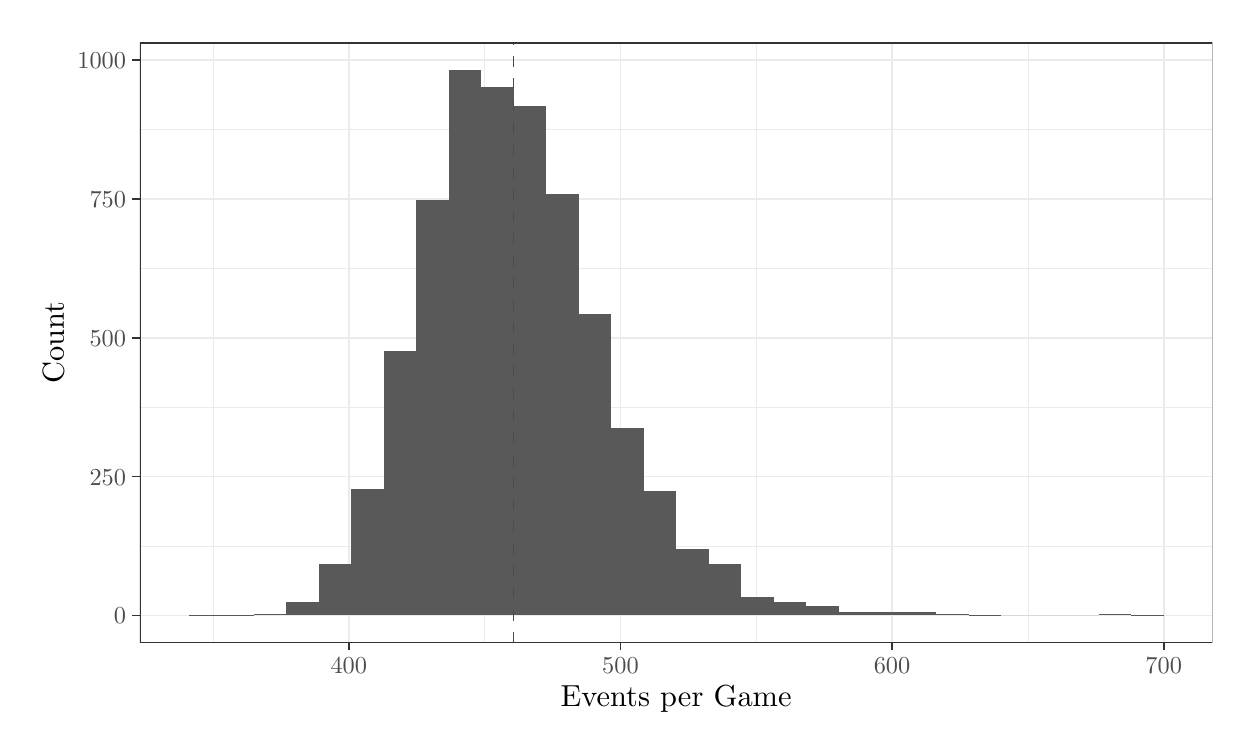
\begin{tikzpicture}[x=1pt,y=1pt]
\definecolor{fillColor}{RGB}{255,255,255}
\path[use as bounding box,fill=fillColor] (0,0) rectangle (433.62,252.94);
\begin{scope}
\path[clip] (  0.00,  0.00) rectangle (433.62,252.94);
\definecolor{drawColor}{RGB}{255,255,255}

\path[draw=drawColor,line width= 0.6pt,line join=round,line cap=round,fill=fillColor] (  0.00,  0.00) rectangle (433.62,252.94);
\end{scope}
\begin{scope}
\path[clip] ( 40.51, 30.69) rectangle (428.12,247.45);
\definecolor{fillColor}{RGB}{255,255,255}

\path[fill=fillColor] ( 40.51, 30.69) rectangle (428.12,247.45);
\definecolor{drawColor}{gray}{0.92}

\path[draw=drawColor,line width= 0.3pt,line join=round] ( 40.51, 65.62) --
	(428.12, 65.62);

\path[draw=drawColor,line width= 0.3pt,line join=round] ( 40.51,115.79) --
	(428.12,115.79);

\path[draw=drawColor,line width= 0.3pt,line join=round] ( 40.51,165.95) --
	(428.12,165.95);

\path[draw=drawColor,line width= 0.3pt,line join=round] ( 40.51,216.12) --
	(428.12,216.12);

\path[draw=drawColor,line width= 0.3pt,line join=round] ( 66.95, 30.69) --
	( 66.95,247.45);

\path[draw=drawColor,line width= 0.3pt,line join=round] (165.11, 30.69) --
	(165.11,247.45);

\path[draw=drawColor,line width= 0.3pt,line join=round] (263.27, 30.69) --
	(263.27,247.45);

\path[draw=drawColor,line width= 0.3pt,line join=round] (361.44, 30.69) --
	(361.44,247.45);

\path[draw=drawColor,line width= 0.6pt,line join=round] ( 40.51, 40.54) --
	(428.12, 40.54);

\path[draw=drawColor,line width= 0.6pt,line join=round] ( 40.51, 90.70) --
	(428.12, 90.70);

\path[draw=drawColor,line width= 0.6pt,line join=round] ( 40.51,140.87) --
	(428.12,140.87);

\path[draw=drawColor,line width= 0.6pt,line join=round] ( 40.51,191.04) --
	(428.12,191.04);

\path[draw=drawColor,line width= 0.6pt,line join=round] ( 40.51,241.20) --
	(428.12,241.20);

\path[draw=drawColor,line width= 0.6pt,line join=round] (116.03, 30.69) --
	(116.03,247.45);

\path[draw=drawColor,line width= 0.6pt,line join=round] (214.19, 30.69) --
	(214.19,247.45);

\path[draw=drawColor,line width= 0.6pt,line join=round] (312.35, 30.69) --
	(312.35,247.45);

\path[draw=drawColor,line width= 0.6pt,line join=round] (410.52, 30.69) --
	(410.52,247.45);
\definecolor{fillColor}{gray}{0.35}

\path[fill=fillColor] ( 58.13, 40.54) rectangle ( 69.87, 40.74);

\path[fill=fillColor] ( 69.87, 40.54) rectangle ( 81.62, 40.74);

\path[fill=fillColor] ( 81.62, 40.54) rectangle ( 93.37, 40.94);

\path[fill=fillColor] ( 93.37, 40.54) rectangle (105.11, 45.35);

\path[fill=fillColor] (105.11, 40.54) rectangle (116.86, 59.20);

\path[fill=fillColor] (116.86, 40.54) rectangle (128.60, 86.29);

\path[fill=fillColor] (128.60, 40.54) rectangle (140.35,136.06);

\path[fill=fillColor] (140.35, 40.54) rectangle (152.09,190.64);

\path[fill=fillColor] (152.09, 40.54) rectangle (163.84,237.59);

\path[fill=fillColor] (163.84, 40.54) rectangle (175.59,231.37);

\path[fill=fillColor] (175.59, 40.54) rectangle (187.33,224.75);

\path[fill=fillColor] (187.33, 40.54) rectangle (199.08,192.84);

\path[fill=fillColor] (199.08, 40.54) rectangle (210.82,149.50);

\path[fill=fillColor] (210.82, 40.54) rectangle (222.57,108.16);

\path[fill=fillColor] (222.57, 40.54) rectangle (234.32, 85.49);

\path[fill=fillColor] (234.32, 40.54) rectangle (246.06, 64.62);

\path[fill=fillColor] (246.06, 40.54) rectangle (257.81, 59.20);

\path[fill=fillColor] (257.81, 40.54) rectangle (269.55, 47.36);

\path[fill=fillColor] (269.55, 40.54) rectangle (281.30, 45.35);

\path[fill=fillColor] (281.30, 40.54) rectangle (293.04, 43.95);

\path[fill=fillColor] (293.04, 40.54) rectangle (304.79, 41.94);

\path[fill=fillColor] (304.79, 40.54) rectangle (316.54, 41.74);

\path[fill=fillColor] (316.54, 40.54) rectangle (328.28, 41.74);

\path[fill=fillColor] (328.28, 40.54) rectangle (340.03, 40.94);

\path[fill=fillColor] (340.03, 40.54) rectangle (351.77, 40.74);

\path[fill=fillColor] (351.77, 40.54) rectangle (363.52, 40.54);

\path[fill=fillColor] (363.52, 40.54) rectangle (375.26, 40.54);

\path[fill=fillColor] (375.26, 40.54) rectangle (387.01, 40.54);

\path[fill=fillColor] (387.01, 40.54) rectangle (398.76, 40.94);

\path[fill=fillColor] (398.76, 40.54) rectangle (410.50, 40.74);
\definecolor{drawColor}{RGB}{255,0,0}

\path[draw=drawColor,line width= 0.6pt,dash pattern=on 4pt off 4pt ,line join=round] (175.60, 30.69) -- (175.60,247.45);
\definecolor{drawColor}{gray}{0.20}

\path[draw=drawColor,line width= 0.6pt,line join=round,line cap=round] ( 40.51, 30.69) rectangle (428.12,247.45);
\end{scope}
\begin{scope}
\path[clip] (  0.00,  0.00) rectangle (433.62,252.94);
\definecolor{drawColor}{gray}{0.30}

\node[text=drawColor,anchor=base east,inner sep=0pt, outer sep=0pt, scale=  0.88] at ( 35.56, 37.51) {0};

\node[text=drawColor,anchor=base east,inner sep=0pt, outer sep=0pt, scale=  0.88] at ( 35.56, 87.67) {250};

\node[text=drawColor,anchor=base east,inner sep=0pt, outer sep=0pt, scale=  0.88] at ( 35.56,137.84) {500};

\node[text=drawColor,anchor=base east,inner sep=0pt, outer sep=0pt, scale=  0.88] at ( 35.56,188.01) {750};

\node[text=drawColor,anchor=base east,inner sep=0pt, outer sep=0pt, scale=  0.88] at ( 35.56,238.17) {1000};
\end{scope}
\begin{scope}
\path[clip] (  0.00,  0.00) rectangle (433.62,252.94);
\definecolor{drawColor}{gray}{0.20}

\path[draw=drawColor,line width= 0.6pt,line join=round] ( 37.76, 40.54) --
	( 40.51, 40.54);

\path[draw=drawColor,line width= 0.6pt,line join=round] ( 37.76, 90.70) --
	( 40.51, 90.70);

\path[draw=drawColor,line width= 0.6pt,line join=round] ( 37.76,140.87) --
	( 40.51,140.87);

\path[draw=drawColor,line width= 0.6pt,line join=round] ( 37.76,191.04) --
	( 40.51,191.04);

\path[draw=drawColor,line width= 0.6pt,line join=round] ( 37.76,241.20) --
	( 40.51,241.20);
\end{scope}
\begin{scope}
\path[clip] (  0.00,  0.00) rectangle (433.62,252.94);
\definecolor{drawColor}{gray}{0.20}

\path[draw=drawColor,line width= 0.6pt,line join=round] (116.03, 27.94) --
	(116.03, 30.69);

\path[draw=drawColor,line width= 0.6pt,line join=round] (214.19, 27.94) --
	(214.19, 30.69);

\path[draw=drawColor,line width= 0.6pt,line join=round] (312.35, 27.94) --
	(312.35, 30.69);

\path[draw=drawColor,line width= 0.6pt,line join=round] (410.52, 27.94) --
	(410.52, 30.69);
\end{scope}
\begin{scope}
\path[clip] (  0.00,  0.00) rectangle (433.62,252.94);
\definecolor{drawColor}{gray}{0.30}

\node[text=drawColor,anchor=base,inner sep=0pt, outer sep=0pt, scale=  0.88] at (116.03, 19.68) {400};

\node[text=drawColor,anchor=base,inner sep=0pt, outer sep=0pt, scale=  0.88] at (214.19, 19.68) {500};

\node[text=drawColor,anchor=base,inner sep=0pt, outer sep=0pt, scale=  0.88] at (312.35, 19.68) {600};

\node[text=drawColor,anchor=base,inner sep=0pt, outer sep=0pt, scale=  0.88] at (410.52, 19.68) {700};
\end{scope}
\begin{scope}
\path[clip] (  0.00,  0.00) rectangle (433.62,252.94);
\definecolor{drawColor}{RGB}{0,0,0}

\node[text=drawColor,anchor=base,inner sep=0pt, outer sep=0pt, scale=  1.10] at (234.32,  7.64) {Events per Game};
\end{scope}
\begin{scope}
\path[clip] (  0.00,  0.00) rectangle (433.62,252.94);
\definecolor{drawColor}{RGB}{0,0,0}

\node[text=drawColor,rotate= 90.00,anchor=base,inner sep=0pt, outer sep=0pt, scale=  1.10] at ( 13.08,139.07) {Count};
\end{scope}
\end{tikzpicture}

	\caption{The distribution of number of events per game with the mean (461) shown in red.}
\end{figure}

\begin{figure}[h]
	% Created by tikzDevice version 0.12.4 on 2024-02-26 09:00:41
% !TEX encoding = UTF-8 Unicode
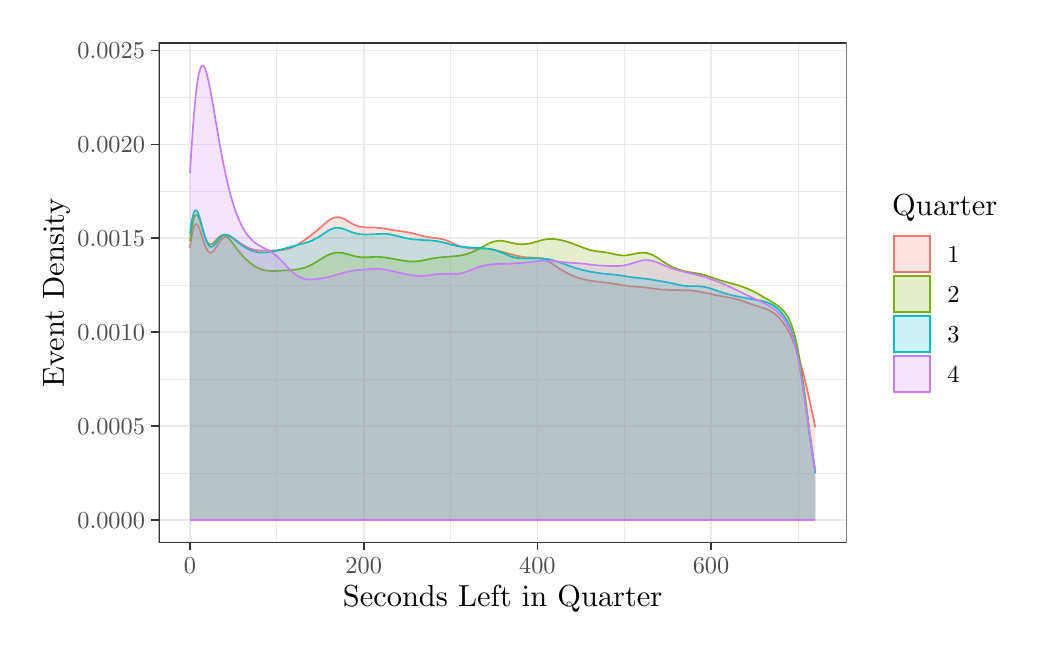
\begin{tikzpicture}[x=1pt,y=1pt]
\definecolor{fillColor}{RGB}{255,255,255}
\path[use as bounding box,fill=fillColor] (0,0) rectangle (361.35,216.81);
\begin{scope}
\path[clip] (  0.00,  0.00) rectangle (361.35,216.81);
\definecolor{drawColor}{RGB}{255,255,255}

\path[draw=drawColor,line width= 0.6pt,line join=round,line cap=round,fill=fillColor] (  0.00,  0.00) rectangle (361.35,216.81);
\end{scope}
\begin{scope}
\path[clip] ( 47.35, 30.69) rectangle (295.91,211.31);
\definecolor{fillColor}{RGB}{255,255,255}

\path[fill=fillColor] ( 47.35, 30.69) rectangle (295.91,211.31);
\definecolor{drawColor}{gray}{0.92}

\path[draw=drawColor,line width= 0.3pt,line join=round] ( 47.35, 55.86) --
	(295.91, 55.86);

\path[draw=drawColor,line width= 0.3pt,line join=round] ( 47.35, 89.79) --
	(295.91, 89.79);

\path[draw=drawColor,line width= 0.3pt,line join=round] ( 47.35,123.72) --
	(295.91,123.72);

\path[draw=drawColor,line width= 0.3pt,line join=round] ( 47.35,157.65) --
	(295.91,157.65);

\path[draw=drawColor,line width= 0.3pt,line join=round] ( 47.35,191.59) --
	(295.91,191.59);

\path[draw=drawColor,line width= 0.3pt,line join=round] ( 90.03, 30.69) --
	( 90.03,211.31);

\path[draw=drawColor,line width= 0.3pt,line join=round] (152.80, 30.69) --
	(152.80,211.31);

\path[draw=drawColor,line width= 0.3pt,line join=round] (215.57, 30.69) --
	(215.57,211.31);

\path[draw=drawColor,line width= 0.3pt,line join=round] (278.33, 30.69) --
	(278.33,211.31);

\path[draw=drawColor,line width= 0.6pt,line join=round] ( 47.35, 38.90) --
	(295.91, 38.90);

\path[draw=drawColor,line width= 0.6pt,line join=round] ( 47.35, 72.83) --
	(295.91, 72.83);

\path[draw=drawColor,line width= 0.6pt,line join=round] ( 47.35,106.76) --
	(295.91,106.76);

\path[draw=drawColor,line width= 0.6pt,line join=round] ( 47.35,140.69) --
	(295.91,140.69);

\path[draw=drawColor,line width= 0.6pt,line join=round] ( 47.35,174.62) --
	(295.91,174.62);

\path[draw=drawColor,line width= 0.6pt,line join=round] ( 47.35,208.55) --
	(295.91,208.55);

\path[draw=drawColor,line width= 0.6pt,line join=round] ( 58.65, 30.69) --
	( 58.65,211.31);

\path[draw=drawColor,line width= 0.6pt,line join=round] (121.42, 30.69) --
	(121.42,211.31);

\path[draw=drawColor,line width= 0.6pt,line join=round] (184.18, 30.69) --
	(184.18,211.31);

\path[draw=drawColor,line width= 0.6pt,line join=round] (246.95, 30.69) --
	(246.95,211.31);
\definecolor{fillColor}{RGB}{248,118,109}

\path[fill=fillColor,fill opacity=0.20] ( 58.65,137.27) --
	( 59.09,140.55) --
	( 59.54,142.96) --
	( 59.98,144.62) --
	( 60.42,145.57) --
	( 60.86,145.87) --
	( 61.30,145.61) --
	( 61.75,144.90) --
	( 62.19,143.83) --
	( 62.63,142.54) --
	( 63.07,141.14) --
	( 63.52,139.76) --
	( 63.96,138.49) --
	( 64.40,137.40) --
	( 64.84,136.54) --
	( 65.28,135.92) --
	( 65.73,135.58) --
	( 66.17,135.49) --
	( 66.61,135.67) --
	( 67.05,136.05) --
	( 67.49,136.57) --
	( 67.94,137.20) --
	( 68.38,137.88) --
	( 68.82,138.58) --
	( 69.26,139.26) --
	( 69.71,139.89) --
	( 70.15,140.42) --
	( 70.59,140.85) --
	( 71.03,141.17) --
	( 71.47,141.39) --
	( 71.92,141.50) --
	( 72.36,141.52) --
	( 72.80,141.45) --
	( 73.24,141.31) --
	( 73.69,141.11) --
	( 74.13,140.85) --
	( 74.57,140.57) --
	( 75.01,140.26) --
	( 75.45,139.95) --
	( 75.90,139.62) --
	( 76.34,139.30) --
	( 76.78,138.99) --
	( 77.22,138.68) --
	( 77.67,138.39) --
	( 78.11,138.12) --
	( 78.55,137.86) --
	( 78.99,137.63) --
	( 79.43,137.41) --
	( 79.88,137.21) --
	( 80.32,137.03) --
	( 80.76,136.87) --
	( 81.20,136.74) --
	( 81.64,136.62) --
	( 82.09,136.52) --
	( 82.53,136.44) --
	( 82.97,136.38) --
	( 83.41,136.33) --
	( 83.86,136.29) --
	( 84.30,136.27) --
	( 84.74,136.25) --
	( 85.18,136.24) --
	( 85.62,136.24) --
	( 86.07,136.24) --
	( 86.51,136.24) --
	( 86.95,136.25) --
	( 87.39,136.26) --
	( 87.84,136.26) --
	( 88.28,136.27) --
	( 88.72,136.28) --
	( 89.16,136.29) --
	( 89.60,136.30) --
	( 90.05,136.31) --
	( 90.49,136.33) --
	( 90.93,136.36) --
	( 91.37,136.40) --
	( 91.82,136.44) --
	( 92.26,136.50) --
	( 92.70,136.57) --
	( 93.14,136.65) --
	( 93.58,136.75) --
	( 94.03,136.87) --
	( 94.47,137.00) --
	( 94.91,137.16) --
	( 95.35,137.32) --
	( 95.80,137.51) --
	( 96.24,137.72) --
	( 96.68,137.94) --
	( 97.12,138.18) --
	( 97.56,138.43) --
	( 98.01,138.70) --
	( 98.45,138.98) --
	( 98.89,139.26) --
	( 99.33,139.56) --
	( 99.77,139.87) --
	(100.22,140.18) --
	(100.66,140.50) --
	(101.10,140.82) --
	(101.54,141.14) --
	(101.99,141.48) --
	(102.43,141.81) --
	(102.87,142.16) --
	(103.31,142.51) --
	(103.75,142.86) --
	(104.20,143.23) --
	(104.64,143.60) --
	(105.08,143.97) --
	(105.52,144.36) --
	(105.97,144.75) --
	(106.41,145.14) --
	(106.85,145.53) --
	(107.29,145.92) --
	(107.73,146.29) --
	(108.18,146.65) --
	(108.62,146.99) --
	(109.06,147.31) --
	(109.50,147.59) --
	(109.95,147.83) --
	(110.39,148.03) --
	(110.83,148.18) --
	(111.27,148.29) --
	(111.71,148.34) --
	(112.16,148.34) --
	(112.60,148.30) --
	(113.04,148.20) --
	(113.48,148.07) --
	(113.92,147.89) --
	(114.37,147.68) --
	(114.81,147.44) --
	(115.25,147.18) --
	(115.69,146.92) --
	(116.14,146.65) --
	(116.58,146.38) --
	(117.02,146.13) --
	(117.46,145.88) --
	(117.90,145.66) --
	(118.35,145.46) --
	(118.79,145.28) --
	(119.23,145.13) --
	(119.67,145.00) --
	(120.12,144.89) --
	(120.56,144.81) --
	(121.00,144.74) --
	(121.44,144.70) --
	(121.88,144.66) --
	(122.33,144.64) --
	(122.77,144.62) --
	(123.21,144.61) --
	(123.65,144.60) --
	(124.10,144.59) --
	(124.54,144.58) --
	(124.98,144.57) --
	(125.42,144.55) --
	(125.86,144.53) --
	(126.31,144.49) --
	(126.75,144.46) --
	(127.19,144.41) --
	(127.63,144.36) --
	(128.08,144.31) --
	(128.52,144.24) --
	(128.96,144.18) --
	(129.40,144.11) --
	(129.84,144.04) --
	(130.29,143.96) --
	(130.73,143.89) --
	(131.17,143.81) --
	(131.61,143.74) --
	(132.05,143.66) --
	(132.50,143.59) --
	(132.94,143.52) --
	(133.38,143.46) --
	(133.82,143.39) --
	(134.27,143.33) --
	(134.71,143.27) --
	(135.15,143.21) --
	(135.59,143.14) --
	(136.03,143.08) --
	(136.48,143.01) --
	(136.92,142.94) --
	(137.36,142.87) --
	(137.80,142.79) --
	(138.25,142.70) --
	(138.69,142.61) --
	(139.13,142.51) --
	(139.57,142.40) --
	(140.01,142.28) --
	(140.46,142.16) --
	(140.90,142.04) --
	(141.34,141.92) --
	(141.78,141.79) --
	(142.23,141.67) --
	(142.67,141.55) --
	(143.11,141.44) --
	(143.55,141.34) --
	(143.99,141.24) --
	(144.44,141.16) --
	(144.88,141.08) --
	(145.32,141.02) --
	(145.76,140.96) --
	(146.20,140.91) --
	(146.65,140.86) --
	(147.09,140.82) --
	(147.53,140.77) --
	(147.97,140.72) --
	(148.42,140.66) --
	(148.86,140.59) --
	(149.30,140.51) --
	(149.74,140.41) --
	(150.18,140.30) --
	(150.63,140.17) --
	(151.07,140.02) --
	(151.51,139.86) --
	(151.95,139.68) --
	(152.40,139.50) --
	(152.84,139.30) --
	(153.28,139.10) --
	(153.72,138.90) --
	(154.16,138.69) --
	(154.61,138.49) --
	(155.05,138.30) --
	(155.49,138.12) --
	(155.93,137.95) --
	(156.38,137.79) --
	(156.82,137.64) --
	(157.26,137.51) --
	(157.70,137.40) --
	(158.14,137.31) --
	(158.59,137.23) --
	(159.03,137.16) --
	(159.47,137.11) --
	(159.91,137.08) --
	(160.36,137.05) --
	(160.80,137.04) --
	(161.24,137.03) --
	(161.68,137.03) --
	(162.12,137.03) --
	(162.57,137.04) --
	(163.01,137.04) --
	(163.45,137.04) --
	(163.89,137.04) --
	(164.33,137.03) --
	(164.78,137.01) --
	(165.22,136.99) --
	(165.66,136.95) --
	(166.10,136.91) --
	(166.55,136.86) --
	(166.99,136.79) --
	(167.43,136.72) --
	(167.87,136.64) --
	(168.31,136.56) --
	(168.76,136.47) --
	(169.20,136.37) --
	(169.64,136.27) --
	(170.08,136.16) --
	(170.53,136.05) --
	(170.97,135.94) --
	(171.41,135.82) --
	(171.85,135.71) --
	(172.29,135.59) --
	(172.74,135.47) --
	(173.18,135.35) --
	(173.62,135.22) --
	(174.06,135.10) --
	(174.51,134.98) --
	(174.95,134.86) --
	(175.39,134.74) --
	(175.83,134.62) --
	(176.27,134.51) --
	(176.72,134.40) --
	(177.16,134.30) --
	(177.60,134.21) --
	(178.04,134.12) --
	(178.48,134.04) --
	(178.93,133.97) --
	(179.37,133.91) --
	(179.81,133.87) --
	(180.25,133.82) --
	(180.70,133.79) --
	(181.14,133.76) --
	(181.58,133.74) --
	(182.02,133.72) --
	(182.46,133.70) --
	(182.91,133.68) --
	(183.35,133.65) --
	(183.79,133.62) --
	(184.23,133.57) --
	(184.68,133.51) --
	(185.12,133.43) --
	(185.56,133.33) --
	(186.00,133.21) --
	(186.44,133.07) --
	(186.89,132.91) --
	(187.33,132.72) --
	(187.77,132.51) --
	(188.21,132.28) --
	(188.66,132.03) --
	(189.10,131.76) --
	(189.54,131.48) --
	(189.98,131.19) --
	(190.42,130.90) --
	(190.87,130.60) --
	(191.31,130.30) --
	(191.75,130.00) --
	(192.19,129.71) --
	(192.64,129.42) --
	(193.08,129.15) --
	(193.52,128.88) --
	(193.96,128.63) --
	(194.40,128.39) --
	(194.85,128.16) --
	(195.29,127.93) --
	(195.73,127.72) --
	(196.17,127.52) --
	(196.61,127.32) --
	(197.06,127.14) --
	(197.50,126.96) --
	(197.94,126.79) --
	(198.38,126.63) --
	(198.83,126.48) --
	(199.27,126.33) --
	(199.71,126.19) --
	(200.15,126.07) --
	(200.59,125.94) --
	(201.04,125.83) --
	(201.48,125.73) --
	(201.92,125.63) --
	(202.36,125.55) --
	(202.81,125.47) --
	(203.25,125.39) --
	(203.69,125.32) --
	(204.13,125.26) --
	(204.57,125.20) --
	(205.02,125.14) --
	(205.46,125.09) --
	(205.90,125.04) --
	(206.34,124.99) --
	(206.79,124.94) --
	(207.23,124.89) --
	(207.67,124.84) --
	(208.11,124.79) --
	(208.55,124.74) --
	(209.00,124.69) --
	(209.44,124.63) --
	(209.88,124.57) --
	(210.32,124.51) --
	(210.76,124.45) --
	(211.21,124.38) --
	(211.65,124.31) --
	(212.09,124.24) --
	(212.53,124.17) --
	(212.98,124.09) --
	(213.42,124.02) --
	(213.86,123.94) --
	(214.30,123.86) --
	(214.74,123.79) --
	(215.19,123.71) --
	(215.63,123.64) --
	(216.07,123.58) --
	(216.51,123.51) --
	(216.96,123.46) --
	(217.40,123.40) --
	(217.84,123.35) --
	(218.28,123.31) --
	(218.72,123.27) --
	(219.17,123.24) --
	(219.61,123.20) --
	(220.05,123.17) --
	(220.49,123.14) --
	(220.94,123.11) --
	(221.38,123.08) --
	(221.82,123.05) --
	(222.26,123.01) --
	(222.70,122.97) --
	(223.15,122.92) --
	(223.59,122.87) --
	(224.03,122.82) --
	(224.47,122.76) --
	(224.92,122.70) --
	(225.36,122.64) --
	(225.80,122.58) --
	(226.24,122.52) --
	(226.68,122.46) --
	(227.13,122.40) --
	(227.57,122.35) --
	(228.01,122.30) --
	(228.45,122.25) --
	(228.89,122.21) --
	(229.34,122.17) --
	(229.78,122.14) --
	(230.22,122.11) --
	(230.66,122.09) --
	(231.11,122.06) --
	(231.55,122.05) --
	(231.99,122.03) --
	(232.43,122.02) --
	(232.87,122.01) --
	(233.32,122.00) --
	(233.76,122.00) --
	(234.20,121.99) --
	(234.64,121.99) --
	(235.09,121.99) --
	(235.53,121.98) --
	(235.97,121.98) --
	(236.41,121.97) --
	(236.85,121.96) --
	(237.30,121.95) --
	(237.74,121.94) --
	(238.18,121.92) --
	(238.62,121.90) --
	(239.07,121.87) --
	(239.51,121.84) --
	(239.95,121.80) --
	(240.39,121.76) --
	(240.83,121.71) --
	(241.28,121.65) --
	(241.72,121.59) --
	(242.16,121.52) --
	(242.60,121.44) --
	(243.05,121.36) --
	(243.49,121.28) --
	(243.93,121.19) --
	(244.37,121.09) --
	(244.81,121.00) --
	(245.26,120.90) --
	(245.70,120.80) --
	(246.14,120.70) --
	(246.58,120.60) --
	(247.02,120.51) --
	(247.47,120.41) --
	(247.91,120.32) --
	(248.35,120.22) --
	(248.79,120.14) --
	(249.24,120.05) --
	(249.68,119.97) --
	(250.12,119.88) --
	(250.56,119.81) --
	(251.00,119.73) --
	(251.45,119.65) --
	(251.89,119.58) --
	(252.33,119.50) --
	(252.77,119.42) --
	(253.22,119.34) --
	(253.66,119.26) --
	(254.10,119.17) --
	(254.54,119.07) --
	(254.98,118.97) --
	(255.43,118.87) --
	(255.87,118.76) --
	(256.31,118.63) --
	(256.75,118.51) --
	(257.20,118.37) --
	(257.64,118.24) --
	(258.08,118.09) --
	(258.52,117.94) --
	(258.96,117.79) --
	(259.41,117.64) --
	(259.85,117.48) --
	(260.29,117.33) --
	(260.73,117.17) --
	(261.17,117.02) --
	(261.62,116.86) --
	(262.06,116.72) --
	(262.50,116.57) --
	(262.94,116.43) --
	(263.39,116.29) --
	(263.83,116.15) --
	(264.27,116.01) --
	(264.71,115.87) --
	(265.15,115.74) --
	(265.60,115.59) --
	(266.04,115.45) --
	(266.48,115.29) --
	(266.92,115.12) --
	(267.37,114.94) --
	(267.81,114.74) --
	(268.25,114.52) --
	(268.69,114.28) --
	(269.13,114.01) --
	(269.58,113.71) --
	(270.02,113.38) --
	(270.46,113.01) --
	(270.90,112.61) --
	(271.35,112.17) --
	(271.79,111.70) --
	(272.23,111.19) --
	(272.67,110.64) --
	(273.11,110.05) --
	(273.56,109.42) --
	(274.00,108.74) --
	(274.44,108.01) --
	(274.88,107.23) --
	(275.33,106.39) --
	(275.77,105.48) --
	(276.21,104.51) --
	(276.65,103.46) --
	(277.09,102.32) --
	(277.54,101.10) --
	(277.98, 99.79) --
	(278.42, 98.39) --
	(278.86, 96.92) --
	(279.30, 95.37) --
	(279.75, 93.75) --
	(280.19, 92.07) --
	(280.63, 90.32) --
	(281.07, 88.52) --
	(281.52, 86.66) --
	(281.96, 84.76) --
	(282.40, 82.81) --
	(282.84, 80.82) --
	(283.28, 78.78) --
	(283.73, 76.70) --
	(284.17, 74.57) --
	(284.61, 72.39) --
	(284.61, 38.90) --
	(284.17, 38.90) --
	(283.73, 38.90) --
	(283.28, 38.90) --
	(282.84, 38.90) --
	(282.40, 38.90) --
	(281.96, 38.90) --
	(281.52, 38.90) --
	(281.07, 38.90) --
	(280.63, 38.90) --
	(280.19, 38.90) --
	(279.75, 38.90) --
	(279.30, 38.90) --
	(278.86, 38.90) --
	(278.42, 38.90) --
	(277.98, 38.90) --
	(277.54, 38.90) --
	(277.09, 38.90) --
	(276.65, 38.90) --
	(276.21, 38.90) --
	(275.77, 38.90) --
	(275.33, 38.90) --
	(274.88, 38.90) --
	(274.44, 38.90) --
	(274.00, 38.90) --
	(273.56, 38.90) --
	(273.11, 38.90) --
	(272.67, 38.90) --
	(272.23, 38.90) --
	(271.79, 38.90) --
	(271.35, 38.90) --
	(270.90, 38.90) --
	(270.46, 38.90) --
	(270.02, 38.90) --
	(269.58, 38.90) --
	(269.13, 38.90) --
	(268.69, 38.90) --
	(268.25, 38.90) --
	(267.81, 38.90) --
	(267.37, 38.90) --
	(266.92, 38.90) --
	(266.48, 38.90) --
	(266.04, 38.90) --
	(265.60, 38.90) --
	(265.15, 38.90) --
	(264.71, 38.90) --
	(264.27, 38.90) --
	(263.83, 38.90) --
	(263.39, 38.90) --
	(262.94, 38.90) --
	(262.50, 38.90) --
	(262.06, 38.90) --
	(261.62, 38.90) --
	(261.17, 38.90) --
	(260.73, 38.90) --
	(260.29, 38.90) --
	(259.85, 38.90) --
	(259.41, 38.90) --
	(258.96, 38.90) --
	(258.52, 38.90) --
	(258.08, 38.90) --
	(257.64, 38.90) --
	(257.20, 38.90) --
	(256.75, 38.90) --
	(256.31, 38.90) --
	(255.87, 38.90) --
	(255.43, 38.90) --
	(254.98, 38.90) --
	(254.54, 38.90) --
	(254.10, 38.90) --
	(253.66, 38.90) --
	(253.22, 38.90) --
	(252.77, 38.90) --
	(252.33, 38.90) --
	(251.89, 38.90) --
	(251.45, 38.90) --
	(251.00, 38.90) --
	(250.56, 38.90) --
	(250.12, 38.90) --
	(249.68, 38.90) --
	(249.24, 38.90) --
	(248.79, 38.90) --
	(248.35, 38.90) --
	(247.91, 38.90) --
	(247.47, 38.90) --
	(247.02, 38.90) --
	(246.58, 38.90) --
	(246.14, 38.90) --
	(245.70, 38.90) --
	(245.26, 38.90) --
	(244.81, 38.90) --
	(244.37, 38.90) --
	(243.93, 38.90) --
	(243.49, 38.90) --
	(243.05, 38.90) --
	(242.60, 38.90) --
	(242.16, 38.90) --
	(241.72, 38.90) --
	(241.28, 38.90) --
	(240.83, 38.90) --
	(240.39, 38.90) --
	(239.95, 38.90) --
	(239.51, 38.90) --
	(239.07, 38.90) --
	(238.62, 38.90) --
	(238.18, 38.90) --
	(237.74, 38.90) --
	(237.30, 38.90) --
	(236.85, 38.90) --
	(236.41, 38.90) --
	(235.97, 38.90) --
	(235.53, 38.90) --
	(235.09, 38.90) --
	(234.64, 38.90) --
	(234.20, 38.90) --
	(233.76, 38.90) --
	(233.32, 38.90) --
	(232.87, 38.90) --
	(232.43, 38.90) --
	(231.99, 38.90) --
	(231.55, 38.90) --
	(231.11, 38.90) --
	(230.66, 38.90) --
	(230.22, 38.90) --
	(229.78, 38.90) --
	(229.34, 38.90) --
	(228.89, 38.90) --
	(228.45, 38.90) --
	(228.01, 38.90) --
	(227.57, 38.90) --
	(227.13, 38.90) --
	(226.68, 38.90) --
	(226.24, 38.90) --
	(225.80, 38.90) --
	(225.36, 38.90) --
	(224.92, 38.90) --
	(224.47, 38.90) --
	(224.03, 38.90) --
	(223.59, 38.90) --
	(223.15, 38.90) --
	(222.70, 38.90) --
	(222.26, 38.90) --
	(221.82, 38.90) --
	(221.38, 38.90) --
	(220.94, 38.90) --
	(220.49, 38.90) --
	(220.05, 38.90) --
	(219.61, 38.90) --
	(219.17, 38.90) --
	(218.72, 38.90) --
	(218.28, 38.90) --
	(217.84, 38.90) --
	(217.40, 38.90) --
	(216.96, 38.90) --
	(216.51, 38.90) --
	(216.07, 38.90) --
	(215.63, 38.90) --
	(215.19, 38.90) --
	(214.74, 38.90) --
	(214.30, 38.90) --
	(213.86, 38.90) --
	(213.42, 38.90) --
	(212.98, 38.90) --
	(212.53, 38.90) --
	(212.09, 38.90) --
	(211.65, 38.90) --
	(211.21, 38.90) --
	(210.76, 38.90) --
	(210.32, 38.90) --
	(209.88, 38.90) --
	(209.44, 38.90) --
	(209.00, 38.90) --
	(208.55, 38.90) --
	(208.11, 38.90) --
	(207.67, 38.90) --
	(207.23, 38.90) --
	(206.79, 38.90) --
	(206.34, 38.90) --
	(205.90, 38.90) --
	(205.46, 38.90) --
	(205.02, 38.90) --
	(204.57, 38.90) --
	(204.13, 38.90) --
	(203.69, 38.90) --
	(203.25, 38.90) --
	(202.81, 38.90) --
	(202.36, 38.90) --
	(201.92, 38.90) --
	(201.48, 38.90) --
	(201.04, 38.90) --
	(200.59, 38.90) --
	(200.15, 38.90) --
	(199.71, 38.90) --
	(199.27, 38.90) --
	(198.83, 38.90) --
	(198.38, 38.90) --
	(197.94, 38.90) --
	(197.50, 38.90) --
	(197.06, 38.90) --
	(196.61, 38.90) --
	(196.17, 38.90) --
	(195.73, 38.90) --
	(195.29, 38.90) --
	(194.85, 38.90) --
	(194.40, 38.90) --
	(193.96, 38.90) --
	(193.52, 38.90) --
	(193.08, 38.90) --
	(192.64, 38.90) --
	(192.19, 38.90) --
	(191.75, 38.90) --
	(191.31, 38.90) --
	(190.87, 38.90) --
	(190.42, 38.90) --
	(189.98, 38.90) --
	(189.54, 38.90) --
	(189.10, 38.90) --
	(188.66, 38.90) --
	(188.21, 38.90) --
	(187.77, 38.90) --
	(187.33, 38.90) --
	(186.89, 38.90) --
	(186.44, 38.90) --
	(186.00, 38.90) --
	(185.56, 38.90) --
	(185.12, 38.90) --
	(184.68, 38.90) --
	(184.23, 38.90) --
	(183.79, 38.90) --
	(183.35, 38.90) --
	(182.91, 38.90) --
	(182.46, 38.90) --
	(182.02, 38.90) --
	(181.58, 38.90) --
	(181.14, 38.90) --
	(180.70, 38.90) --
	(180.25, 38.90) --
	(179.81, 38.90) --
	(179.37, 38.90) --
	(178.93, 38.90) --
	(178.48, 38.90) --
	(178.04, 38.90) --
	(177.60, 38.90) --
	(177.16, 38.90) --
	(176.72, 38.90) --
	(176.27, 38.90) --
	(175.83, 38.90) --
	(175.39, 38.90) --
	(174.95, 38.90) --
	(174.51, 38.90) --
	(174.06, 38.90) --
	(173.62, 38.90) --
	(173.18, 38.90) --
	(172.74, 38.90) --
	(172.29, 38.90) --
	(171.85, 38.90) --
	(171.41, 38.90) --
	(170.97, 38.90) --
	(170.53, 38.90) --
	(170.08, 38.90) --
	(169.64, 38.90) --
	(169.20, 38.90) --
	(168.76, 38.90) --
	(168.31, 38.90) --
	(167.87, 38.90) --
	(167.43, 38.90) --
	(166.99, 38.90) --
	(166.55, 38.90) --
	(166.10, 38.90) --
	(165.66, 38.90) --
	(165.22, 38.90) --
	(164.78, 38.90) --
	(164.33, 38.90) --
	(163.89, 38.90) --
	(163.45, 38.90) --
	(163.01, 38.90) --
	(162.57, 38.90) --
	(162.12, 38.90) --
	(161.68, 38.90) --
	(161.24, 38.90) --
	(160.80, 38.90) --
	(160.36, 38.90) --
	(159.91, 38.90) --
	(159.47, 38.90) --
	(159.03, 38.90) --
	(158.59, 38.90) --
	(158.14, 38.90) --
	(157.70, 38.90) --
	(157.26, 38.90) --
	(156.82, 38.90) --
	(156.38, 38.90) --
	(155.93, 38.90) --
	(155.49, 38.90) --
	(155.05, 38.90) --
	(154.61, 38.90) --
	(154.16, 38.90) --
	(153.72, 38.90) --
	(153.28, 38.90) --
	(152.84, 38.90) --
	(152.40, 38.90) --
	(151.95, 38.90) --
	(151.51, 38.90) --
	(151.07, 38.90) --
	(150.63, 38.90) --
	(150.18, 38.90) --
	(149.74, 38.90) --
	(149.30, 38.90) --
	(148.86, 38.90) --
	(148.42, 38.90) --
	(147.97, 38.90) --
	(147.53, 38.90) --
	(147.09, 38.90) --
	(146.65, 38.90) --
	(146.20, 38.90) --
	(145.76, 38.90) --
	(145.32, 38.90) --
	(144.88, 38.90) --
	(144.44, 38.90) --
	(143.99, 38.90) --
	(143.55, 38.90) --
	(143.11, 38.90) --
	(142.67, 38.90) --
	(142.23, 38.90) --
	(141.78, 38.90) --
	(141.34, 38.90) --
	(140.90, 38.90) --
	(140.46, 38.90) --
	(140.01, 38.90) --
	(139.57, 38.90) --
	(139.13, 38.90) --
	(138.69, 38.90) --
	(138.25, 38.90) --
	(137.80, 38.90) --
	(137.36, 38.90) --
	(136.92, 38.90) --
	(136.48, 38.90) --
	(136.03, 38.90) --
	(135.59, 38.90) --
	(135.15, 38.90) --
	(134.71, 38.90) --
	(134.27, 38.90) --
	(133.82, 38.90) --
	(133.38, 38.90) --
	(132.94, 38.90) --
	(132.50, 38.90) --
	(132.05, 38.90) --
	(131.61, 38.90) --
	(131.17, 38.90) --
	(130.73, 38.90) --
	(130.29, 38.90) --
	(129.84, 38.90) --
	(129.40, 38.90) --
	(128.96, 38.90) --
	(128.52, 38.90) --
	(128.08, 38.90) --
	(127.63, 38.90) --
	(127.19, 38.90) --
	(126.75, 38.90) --
	(126.31, 38.90) --
	(125.86, 38.90) --
	(125.42, 38.90) --
	(124.98, 38.90) --
	(124.54, 38.90) --
	(124.10, 38.90) --
	(123.65, 38.90) --
	(123.21, 38.90) --
	(122.77, 38.90) --
	(122.33, 38.90) --
	(121.88, 38.90) --
	(121.44, 38.90) --
	(121.00, 38.90) --
	(120.56, 38.90) --
	(120.12, 38.90) --
	(119.67, 38.90) --
	(119.23, 38.90) --
	(118.79, 38.90) --
	(118.35, 38.90) --
	(117.90, 38.90) --
	(117.46, 38.90) --
	(117.02, 38.90) --
	(116.58, 38.90) --
	(116.14, 38.90) --
	(115.69, 38.90) --
	(115.25, 38.90) --
	(114.81, 38.90) --
	(114.37, 38.90) --
	(113.92, 38.90) --
	(113.48, 38.90) --
	(113.04, 38.90) --
	(112.60, 38.90) --
	(112.16, 38.90) --
	(111.71, 38.90) --
	(111.27, 38.90) --
	(110.83, 38.90) --
	(110.39, 38.90) --
	(109.95, 38.90) --
	(109.50, 38.90) --
	(109.06, 38.90) --
	(108.62, 38.90) --
	(108.18, 38.90) --
	(107.73, 38.90) --
	(107.29, 38.90) --
	(106.85, 38.90) --
	(106.41, 38.90) --
	(105.97, 38.90) --
	(105.52, 38.90) --
	(105.08, 38.90) --
	(104.64, 38.90) --
	(104.20, 38.90) --
	(103.75, 38.90) --
	(103.31, 38.90) --
	(102.87, 38.90) --
	(102.43, 38.90) --
	(101.99, 38.90) --
	(101.54, 38.90) --
	(101.10, 38.90) --
	(100.66, 38.90) --
	(100.22, 38.90) --
	( 99.77, 38.90) --
	( 99.33, 38.90) --
	( 98.89, 38.90) --
	( 98.45, 38.90) --
	( 98.01, 38.90) --
	( 97.56, 38.90) --
	( 97.12, 38.90) --
	( 96.68, 38.90) --
	( 96.24, 38.90) --
	( 95.80, 38.90) --
	( 95.35, 38.90) --
	( 94.91, 38.90) --
	( 94.47, 38.90) --
	( 94.03, 38.90) --
	( 93.58, 38.90) --
	( 93.14, 38.90) --
	( 92.70, 38.90) --
	( 92.26, 38.90) --
	( 91.82, 38.90) --
	( 91.37, 38.90) --
	( 90.93, 38.90) --
	( 90.49, 38.90) --
	( 90.05, 38.90) --
	( 89.60, 38.90) --
	( 89.16, 38.90) --
	( 88.72, 38.90) --
	( 88.28, 38.90) --
	( 87.84, 38.90) --
	( 87.39, 38.90) --
	( 86.95, 38.90) --
	( 86.51, 38.90) --
	( 86.07, 38.90) --
	( 85.62, 38.90) --
	( 85.18, 38.90) --
	( 84.74, 38.90) --
	( 84.30, 38.90) --
	( 83.86, 38.90) --
	( 83.41, 38.90) --
	( 82.97, 38.90) --
	( 82.53, 38.90) --
	( 82.09, 38.90) --
	( 81.64, 38.90) --
	( 81.20, 38.90) --
	( 80.76, 38.90) --
	( 80.32, 38.90) --
	( 79.88, 38.90) --
	( 79.43, 38.90) --
	( 78.99, 38.90) --
	( 78.55, 38.90) --
	( 78.11, 38.90) --
	( 77.67, 38.90) --
	( 77.22, 38.90) --
	( 76.78, 38.90) --
	( 76.34, 38.90) --
	( 75.90, 38.90) --
	( 75.45, 38.90) --
	( 75.01, 38.90) --
	( 74.57, 38.90) --
	( 74.13, 38.90) --
	( 73.69, 38.90) --
	( 73.24, 38.90) --
	( 72.80, 38.90) --
	( 72.36, 38.90) --
	( 71.92, 38.90) --
	( 71.47, 38.90) --
	( 71.03, 38.90) --
	( 70.59, 38.90) --
	( 70.15, 38.90) --
	( 69.71, 38.90) --
	( 69.26, 38.90) --
	( 68.82, 38.90) --
	( 68.38, 38.90) --
	( 67.94, 38.90) --
	( 67.49, 38.90) --
	( 67.05, 38.90) --
	( 66.61, 38.90) --
	( 66.17, 38.90) --
	( 65.73, 38.90) --
	( 65.28, 38.90) --
	( 64.84, 38.90) --
	( 64.40, 38.90) --
	( 63.96, 38.90) --
	( 63.52, 38.90) --
	( 63.07, 38.90) --
	( 62.63, 38.90) --
	( 62.19, 38.90) --
	( 61.75, 38.90) --
	( 61.30, 38.90) --
	( 60.86, 38.90) --
	( 60.42, 38.90) --
	( 59.98, 38.90) --
	( 59.54, 38.90) --
	( 59.09, 38.90) --
	( 58.65, 38.90) --
	cycle;
\definecolor{drawColor}{RGB}{248,118,109}

\path[draw=drawColor,line width= 0.6pt,line join=round] ( 58.65,137.27) --
	( 59.09,140.55) --
	( 59.54,142.96) --
	( 59.98,144.62) --
	( 60.42,145.57) --
	( 60.86,145.87) --
	( 61.30,145.61) --
	( 61.75,144.90) --
	( 62.19,143.83) --
	( 62.63,142.54) --
	( 63.07,141.14) --
	( 63.52,139.76) --
	( 63.96,138.49) --
	( 64.40,137.40) --
	( 64.84,136.54) --
	( 65.28,135.92) --
	( 65.73,135.58) --
	( 66.17,135.49) --
	( 66.61,135.67) --
	( 67.05,136.05) --
	( 67.49,136.57) --
	( 67.94,137.20) --
	( 68.38,137.88) --
	( 68.82,138.58) --
	( 69.26,139.26) --
	( 69.71,139.89) --
	( 70.15,140.42) --
	( 70.59,140.85) --
	( 71.03,141.17) --
	( 71.47,141.39) --
	( 71.92,141.50) --
	( 72.36,141.52) --
	( 72.80,141.45) --
	( 73.24,141.31) --
	( 73.69,141.11) --
	( 74.13,140.85) --
	( 74.57,140.57) --
	( 75.01,140.26) --
	( 75.45,139.95) --
	( 75.90,139.62) --
	( 76.34,139.30) --
	( 76.78,138.99) --
	( 77.22,138.68) --
	( 77.67,138.39) --
	( 78.11,138.12) --
	( 78.55,137.86) --
	( 78.99,137.63) --
	( 79.43,137.41) --
	( 79.88,137.21) --
	( 80.32,137.03) --
	( 80.76,136.87) --
	( 81.20,136.74) --
	( 81.64,136.62) --
	( 82.09,136.52) --
	( 82.53,136.44) --
	( 82.97,136.38) --
	( 83.41,136.33) --
	( 83.86,136.29) --
	( 84.30,136.27) --
	( 84.74,136.25) --
	( 85.18,136.24) --
	( 85.62,136.24) --
	( 86.07,136.24) --
	( 86.51,136.24) --
	( 86.95,136.25) --
	( 87.39,136.26) --
	( 87.84,136.26) --
	( 88.28,136.27) --
	( 88.72,136.28) --
	( 89.16,136.29) --
	( 89.60,136.30) --
	( 90.05,136.31) --
	( 90.49,136.33) --
	( 90.93,136.36) --
	( 91.37,136.40) --
	( 91.82,136.44) --
	( 92.26,136.50) --
	( 92.70,136.57) --
	( 93.14,136.65) --
	( 93.58,136.75) --
	( 94.03,136.87) --
	( 94.47,137.00) --
	( 94.91,137.16) --
	( 95.35,137.32) --
	( 95.80,137.51) --
	( 96.24,137.72) --
	( 96.68,137.94) --
	( 97.12,138.18) --
	( 97.56,138.43) --
	( 98.01,138.70) --
	( 98.45,138.98) --
	( 98.89,139.26) --
	( 99.33,139.56) --
	( 99.77,139.87) --
	(100.22,140.18) --
	(100.66,140.50) --
	(101.10,140.82) --
	(101.54,141.14) --
	(101.99,141.48) --
	(102.43,141.81) --
	(102.87,142.16) --
	(103.31,142.51) --
	(103.75,142.86) --
	(104.20,143.23) --
	(104.64,143.60) --
	(105.08,143.97) --
	(105.52,144.36) --
	(105.97,144.75) --
	(106.41,145.14) --
	(106.85,145.53) --
	(107.29,145.92) --
	(107.73,146.29) --
	(108.18,146.65) --
	(108.62,146.99) --
	(109.06,147.31) --
	(109.50,147.59) --
	(109.95,147.83) --
	(110.39,148.03) --
	(110.83,148.18) --
	(111.27,148.29) --
	(111.71,148.34) --
	(112.16,148.34) --
	(112.60,148.30) --
	(113.04,148.20) --
	(113.48,148.07) --
	(113.92,147.89) --
	(114.37,147.68) --
	(114.81,147.44) --
	(115.25,147.18) --
	(115.69,146.92) --
	(116.14,146.65) --
	(116.58,146.38) --
	(117.02,146.13) --
	(117.46,145.88) --
	(117.90,145.66) --
	(118.35,145.46) --
	(118.79,145.28) --
	(119.23,145.13) --
	(119.67,145.00) --
	(120.12,144.89) --
	(120.56,144.81) --
	(121.00,144.74) --
	(121.44,144.70) --
	(121.88,144.66) --
	(122.33,144.64) --
	(122.77,144.62) --
	(123.21,144.61) --
	(123.65,144.60) --
	(124.10,144.59) --
	(124.54,144.58) --
	(124.98,144.57) --
	(125.42,144.55) --
	(125.86,144.53) --
	(126.31,144.49) --
	(126.75,144.46) --
	(127.19,144.41) --
	(127.63,144.36) --
	(128.08,144.31) --
	(128.52,144.24) --
	(128.96,144.18) --
	(129.40,144.11) --
	(129.84,144.04) --
	(130.29,143.96) --
	(130.73,143.89) --
	(131.17,143.81) --
	(131.61,143.74) --
	(132.05,143.66) --
	(132.50,143.59) --
	(132.94,143.52) --
	(133.38,143.46) --
	(133.82,143.39) --
	(134.27,143.33) --
	(134.71,143.27) --
	(135.15,143.21) --
	(135.59,143.14) --
	(136.03,143.08) --
	(136.48,143.01) --
	(136.92,142.94) --
	(137.36,142.87) --
	(137.80,142.79) --
	(138.25,142.70) --
	(138.69,142.61) --
	(139.13,142.51) --
	(139.57,142.40) --
	(140.01,142.28) --
	(140.46,142.16) --
	(140.90,142.04) --
	(141.34,141.92) --
	(141.78,141.79) --
	(142.23,141.67) --
	(142.67,141.55) --
	(143.11,141.44) --
	(143.55,141.34) --
	(143.99,141.24) --
	(144.44,141.16) --
	(144.88,141.08) --
	(145.32,141.02) --
	(145.76,140.96) --
	(146.20,140.91) --
	(146.65,140.86) --
	(147.09,140.82) --
	(147.53,140.77) --
	(147.97,140.72) --
	(148.42,140.66) --
	(148.86,140.59) --
	(149.30,140.51) --
	(149.74,140.41) --
	(150.18,140.30) --
	(150.63,140.17) --
	(151.07,140.02) --
	(151.51,139.86) --
	(151.95,139.68) --
	(152.40,139.50) --
	(152.84,139.30) --
	(153.28,139.10) --
	(153.72,138.90) --
	(154.16,138.69) --
	(154.61,138.49) --
	(155.05,138.30) --
	(155.49,138.12) --
	(155.93,137.95) --
	(156.38,137.79) --
	(156.82,137.64) --
	(157.26,137.51) --
	(157.70,137.40) --
	(158.14,137.31) --
	(158.59,137.23) --
	(159.03,137.16) --
	(159.47,137.11) --
	(159.91,137.08) --
	(160.36,137.05) --
	(160.80,137.04) --
	(161.24,137.03) --
	(161.68,137.03) --
	(162.12,137.03) --
	(162.57,137.04) --
	(163.01,137.04) --
	(163.45,137.04) --
	(163.89,137.04) --
	(164.33,137.03) --
	(164.78,137.01) --
	(165.22,136.99) --
	(165.66,136.95) --
	(166.10,136.91) --
	(166.55,136.86) --
	(166.99,136.79) --
	(167.43,136.72) --
	(167.87,136.64) --
	(168.31,136.56) --
	(168.76,136.47) --
	(169.20,136.37) --
	(169.64,136.27) --
	(170.08,136.16) --
	(170.53,136.05) --
	(170.97,135.94) --
	(171.41,135.82) --
	(171.85,135.71) --
	(172.29,135.59) --
	(172.74,135.47) --
	(173.18,135.35) --
	(173.62,135.22) --
	(174.06,135.10) --
	(174.51,134.98) --
	(174.95,134.86) --
	(175.39,134.74) --
	(175.83,134.62) --
	(176.27,134.51) --
	(176.72,134.40) --
	(177.16,134.30) --
	(177.60,134.21) --
	(178.04,134.12) --
	(178.48,134.04) --
	(178.93,133.97) --
	(179.37,133.91) --
	(179.81,133.87) --
	(180.25,133.82) --
	(180.70,133.79) --
	(181.14,133.76) --
	(181.58,133.74) --
	(182.02,133.72) --
	(182.46,133.70) --
	(182.91,133.68) --
	(183.35,133.65) --
	(183.79,133.62) --
	(184.23,133.57) --
	(184.68,133.51) --
	(185.12,133.43) --
	(185.56,133.33) --
	(186.00,133.21) --
	(186.44,133.07) --
	(186.89,132.91) --
	(187.33,132.72) --
	(187.77,132.51) --
	(188.21,132.28) --
	(188.66,132.03) --
	(189.10,131.76) --
	(189.54,131.48) --
	(189.98,131.19) --
	(190.42,130.90) --
	(190.87,130.60) --
	(191.31,130.30) --
	(191.75,130.00) --
	(192.19,129.71) --
	(192.64,129.42) --
	(193.08,129.15) --
	(193.52,128.88) --
	(193.96,128.63) --
	(194.40,128.39) --
	(194.85,128.16) --
	(195.29,127.93) --
	(195.73,127.72) --
	(196.17,127.52) --
	(196.61,127.32) --
	(197.06,127.14) --
	(197.50,126.96) --
	(197.94,126.79) --
	(198.38,126.63) --
	(198.83,126.48) --
	(199.27,126.33) --
	(199.71,126.19) --
	(200.15,126.07) --
	(200.59,125.94) --
	(201.04,125.83) --
	(201.48,125.73) --
	(201.92,125.63) --
	(202.36,125.55) --
	(202.81,125.47) --
	(203.25,125.39) --
	(203.69,125.32) --
	(204.13,125.26) --
	(204.57,125.20) --
	(205.02,125.14) --
	(205.46,125.09) --
	(205.90,125.04) --
	(206.34,124.99) --
	(206.79,124.94) --
	(207.23,124.89) --
	(207.67,124.84) --
	(208.11,124.79) --
	(208.55,124.74) --
	(209.00,124.69) --
	(209.44,124.63) --
	(209.88,124.57) --
	(210.32,124.51) --
	(210.76,124.45) --
	(211.21,124.38) --
	(211.65,124.31) --
	(212.09,124.24) --
	(212.53,124.17) --
	(212.98,124.09) --
	(213.42,124.02) --
	(213.86,123.94) --
	(214.30,123.86) --
	(214.74,123.79) --
	(215.19,123.71) --
	(215.63,123.64) --
	(216.07,123.58) --
	(216.51,123.51) --
	(216.96,123.46) --
	(217.40,123.40) --
	(217.84,123.35) --
	(218.28,123.31) --
	(218.72,123.27) --
	(219.17,123.24) --
	(219.61,123.20) --
	(220.05,123.17) --
	(220.49,123.14) --
	(220.94,123.11) --
	(221.38,123.08) --
	(221.82,123.05) --
	(222.26,123.01) --
	(222.70,122.97) --
	(223.15,122.92) --
	(223.59,122.87) --
	(224.03,122.82) --
	(224.47,122.76) --
	(224.92,122.70) --
	(225.36,122.64) --
	(225.80,122.58) --
	(226.24,122.52) --
	(226.68,122.46) --
	(227.13,122.40) --
	(227.57,122.35) --
	(228.01,122.30) --
	(228.45,122.25) --
	(228.89,122.21) --
	(229.34,122.17) --
	(229.78,122.14) --
	(230.22,122.11) --
	(230.66,122.09) --
	(231.11,122.06) --
	(231.55,122.05) --
	(231.99,122.03) --
	(232.43,122.02) --
	(232.87,122.01) --
	(233.32,122.00) --
	(233.76,122.00) --
	(234.20,121.99) --
	(234.64,121.99) --
	(235.09,121.99) --
	(235.53,121.98) --
	(235.97,121.98) --
	(236.41,121.97) --
	(236.85,121.96) --
	(237.30,121.95) --
	(237.74,121.94) --
	(238.18,121.92) --
	(238.62,121.90) --
	(239.07,121.87) --
	(239.51,121.84) --
	(239.95,121.80) --
	(240.39,121.76) --
	(240.83,121.71) --
	(241.28,121.65) --
	(241.72,121.59) --
	(242.16,121.52) --
	(242.60,121.44) --
	(243.05,121.36) --
	(243.49,121.28) --
	(243.93,121.19) --
	(244.37,121.09) --
	(244.81,121.00) --
	(245.26,120.90) --
	(245.70,120.80) --
	(246.14,120.70) --
	(246.58,120.60) --
	(247.02,120.51) --
	(247.47,120.41) --
	(247.91,120.32) --
	(248.35,120.22) --
	(248.79,120.14) --
	(249.24,120.05) --
	(249.68,119.97) --
	(250.12,119.88) --
	(250.56,119.81) --
	(251.00,119.73) --
	(251.45,119.65) --
	(251.89,119.58) --
	(252.33,119.50) --
	(252.77,119.42) --
	(253.22,119.34) --
	(253.66,119.26) --
	(254.10,119.17) --
	(254.54,119.07) --
	(254.98,118.97) --
	(255.43,118.87) --
	(255.87,118.76) --
	(256.31,118.63) --
	(256.75,118.51) --
	(257.20,118.37) --
	(257.64,118.24) --
	(258.08,118.09) --
	(258.52,117.94) --
	(258.96,117.79) --
	(259.41,117.64) --
	(259.85,117.48) --
	(260.29,117.33) --
	(260.73,117.17) --
	(261.17,117.02) --
	(261.62,116.86) --
	(262.06,116.72) --
	(262.50,116.57) --
	(262.94,116.43) --
	(263.39,116.29) --
	(263.83,116.15) --
	(264.27,116.01) --
	(264.71,115.87) --
	(265.15,115.74) --
	(265.60,115.59) --
	(266.04,115.45) --
	(266.48,115.29) --
	(266.92,115.12) --
	(267.37,114.94) --
	(267.81,114.74) --
	(268.25,114.52) --
	(268.69,114.28) --
	(269.13,114.01) --
	(269.58,113.71) --
	(270.02,113.38) --
	(270.46,113.01) --
	(270.90,112.61) --
	(271.35,112.17) --
	(271.79,111.70) --
	(272.23,111.19) --
	(272.67,110.64) --
	(273.11,110.05) --
	(273.56,109.42) --
	(274.00,108.74) --
	(274.44,108.01) --
	(274.88,107.23) --
	(275.33,106.39) --
	(275.77,105.48) --
	(276.21,104.51) --
	(276.65,103.46) --
	(277.09,102.32) --
	(277.54,101.10) --
	(277.98, 99.79) --
	(278.42, 98.39) --
	(278.86, 96.92) --
	(279.30, 95.37) --
	(279.75, 93.75) --
	(280.19, 92.07) --
	(280.63, 90.32) --
	(281.07, 88.52) --
	(281.52, 86.66) --
	(281.96, 84.76) --
	(282.40, 82.81) --
	(282.84, 80.82) --
	(283.28, 78.78) --
	(283.73, 76.70) --
	(284.17, 74.57) --
	(284.61, 72.39);

\path[draw=drawColor,line width= 0.6pt,line join=round] (284.61, 38.90) --
	(284.17, 38.90) --
	(283.73, 38.90) --
	(283.28, 38.90) --
	(282.84, 38.90) --
	(282.40, 38.90) --
	(281.96, 38.90) --
	(281.52, 38.90) --
	(281.07, 38.90) --
	(280.63, 38.90) --
	(280.19, 38.90) --
	(279.75, 38.90) --
	(279.30, 38.90) --
	(278.86, 38.90) --
	(278.42, 38.90) --
	(277.98, 38.90) --
	(277.54, 38.90) --
	(277.09, 38.90) --
	(276.65, 38.90) --
	(276.21, 38.90) --
	(275.77, 38.90) --
	(275.33, 38.90) --
	(274.88, 38.90) --
	(274.44, 38.90) --
	(274.00, 38.90) --
	(273.56, 38.90) --
	(273.11, 38.90) --
	(272.67, 38.90) --
	(272.23, 38.90) --
	(271.79, 38.90) --
	(271.35, 38.90) --
	(270.90, 38.90) --
	(270.46, 38.90) --
	(270.02, 38.90) --
	(269.58, 38.90) --
	(269.13, 38.90) --
	(268.69, 38.90) --
	(268.25, 38.90) --
	(267.81, 38.90) --
	(267.37, 38.90) --
	(266.92, 38.90) --
	(266.48, 38.90) --
	(266.04, 38.90) --
	(265.60, 38.90) --
	(265.15, 38.90) --
	(264.71, 38.90) --
	(264.27, 38.90) --
	(263.83, 38.90) --
	(263.39, 38.90) --
	(262.94, 38.90) --
	(262.50, 38.90) --
	(262.06, 38.90) --
	(261.62, 38.90) --
	(261.17, 38.90) --
	(260.73, 38.90) --
	(260.29, 38.90) --
	(259.85, 38.90) --
	(259.41, 38.90) --
	(258.96, 38.90) --
	(258.52, 38.90) --
	(258.08, 38.90) --
	(257.64, 38.90) --
	(257.20, 38.90) --
	(256.75, 38.90) --
	(256.31, 38.90) --
	(255.87, 38.90) --
	(255.43, 38.90) --
	(254.98, 38.90) --
	(254.54, 38.90) --
	(254.10, 38.90) --
	(253.66, 38.90) --
	(253.22, 38.90) --
	(252.77, 38.90) --
	(252.33, 38.90) --
	(251.89, 38.90) --
	(251.45, 38.90) --
	(251.00, 38.90) --
	(250.56, 38.90) --
	(250.12, 38.90) --
	(249.68, 38.90) --
	(249.24, 38.90) --
	(248.79, 38.90) --
	(248.35, 38.90) --
	(247.91, 38.90) --
	(247.47, 38.90) --
	(247.02, 38.90) --
	(246.58, 38.90) --
	(246.14, 38.90) --
	(245.70, 38.90) --
	(245.26, 38.90) --
	(244.81, 38.90) --
	(244.37, 38.90) --
	(243.93, 38.90) --
	(243.49, 38.90) --
	(243.05, 38.90) --
	(242.60, 38.90) --
	(242.16, 38.90) --
	(241.72, 38.90) --
	(241.28, 38.90) --
	(240.83, 38.90) --
	(240.39, 38.90) --
	(239.95, 38.90) --
	(239.51, 38.90) --
	(239.07, 38.90) --
	(238.62, 38.90) --
	(238.18, 38.90) --
	(237.74, 38.90) --
	(237.30, 38.90) --
	(236.85, 38.90) --
	(236.41, 38.90) --
	(235.97, 38.90) --
	(235.53, 38.90) --
	(235.09, 38.90) --
	(234.64, 38.90) --
	(234.20, 38.90) --
	(233.76, 38.90) --
	(233.32, 38.90) --
	(232.87, 38.90) --
	(232.43, 38.90) --
	(231.99, 38.90) --
	(231.55, 38.90) --
	(231.11, 38.90) --
	(230.66, 38.90) --
	(230.22, 38.90) --
	(229.78, 38.90) --
	(229.34, 38.90) --
	(228.89, 38.90) --
	(228.45, 38.90) --
	(228.01, 38.90) --
	(227.57, 38.90) --
	(227.13, 38.90) --
	(226.68, 38.90) --
	(226.24, 38.90) --
	(225.80, 38.90) --
	(225.36, 38.90) --
	(224.92, 38.90) --
	(224.47, 38.90) --
	(224.03, 38.90) --
	(223.59, 38.90) --
	(223.15, 38.90) --
	(222.70, 38.90) --
	(222.26, 38.90) --
	(221.82, 38.90) --
	(221.38, 38.90) --
	(220.94, 38.90) --
	(220.49, 38.90) --
	(220.05, 38.90) --
	(219.61, 38.90) --
	(219.17, 38.90) --
	(218.72, 38.90) --
	(218.28, 38.90) --
	(217.84, 38.90) --
	(217.40, 38.90) --
	(216.96, 38.90) --
	(216.51, 38.90) --
	(216.07, 38.90) --
	(215.63, 38.90) --
	(215.19, 38.90) --
	(214.74, 38.90) --
	(214.30, 38.90) --
	(213.86, 38.90) --
	(213.42, 38.90) --
	(212.98, 38.90) --
	(212.53, 38.90) --
	(212.09, 38.90) --
	(211.65, 38.90) --
	(211.21, 38.90) --
	(210.76, 38.90) --
	(210.32, 38.90) --
	(209.88, 38.90) --
	(209.44, 38.90) --
	(209.00, 38.90) --
	(208.55, 38.90) --
	(208.11, 38.90) --
	(207.67, 38.90) --
	(207.23, 38.90) --
	(206.79, 38.90) --
	(206.34, 38.90) --
	(205.90, 38.90) --
	(205.46, 38.90) --
	(205.02, 38.90) --
	(204.57, 38.90) --
	(204.13, 38.90) --
	(203.69, 38.90) --
	(203.25, 38.90) --
	(202.81, 38.90) --
	(202.36, 38.90) --
	(201.92, 38.90) --
	(201.48, 38.90) --
	(201.04, 38.90) --
	(200.59, 38.90) --
	(200.15, 38.90) --
	(199.71, 38.90) --
	(199.27, 38.90) --
	(198.83, 38.90) --
	(198.38, 38.90) --
	(197.94, 38.90) --
	(197.50, 38.90) --
	(197.06, 38.90) --
	(196.61, 38.90) --
	(196.17, 38.90) --
	(195.73, 38.90) --
	(195.29, 38.90) --
	(194.85, 38.90) --
	(194.40, 38.90) --
	(193.96, 38.90) --
	(193.52, 38.90) --
	(193.08, 38.90) --
	(192.64, 38.90) --
	(192.19, 38.90) --
	(191.75, 38.90) --
	(191.31, 38.90) --
	(190.87, 38.90) --
	(190.42, 38.90) --
	(189.98, 38.90) --
	(189.54, 38.90) --
	(189.10, 38.90) --
	(188.66, 38.90) --
	(188.21, 38.90) --
	(187.77, 38.90) --
	(187.33, 38.90) --
	(186.89, 38.90) --
	(186.44, 38.90) --
	(186.00, 38.90) --
	(185.56, 38.90) --
	(185.12, 38.90) --
	(184.68, 38.90) --
	(184.23, 38.90) --
	(183.79, 38.90) --
	(183.35, 38.90) --
	(182.91, 38.90) --
	(182.46, 38.90) --
	(182.02, 38.90) --
	(181.58, 38.90) --
	(181.14, 38.90) --
	(180.70, 38.90) --
	(180.25, 38.90) --
	(179.81, 38.90) --
	(179.37, 38.90) --
	(178.93, 38.90) --
	(178.48, 38.90) --
	(178.04, 38.90) --
	(177.60, 38.90) --
	(177.16, 38.90) --
	(176.72, 38.90) --
	(176.27, 38.90) --
	(175.83, 38.90) --
	(175.39, 38.90) --
	(174.95, 38.90) --
	(174.51, 38.90) --
	(174.06, 38.90) --
	(173.62, 38.90) --
	(173.18, 38.90) --
	(172.74, 38.90) --
	(172.29, 38.90) --
	(171.85, 38.90) --
	(171.41, 38.90) --
	(170.97, 38.90) --
	(170.53, 38.90) --
	(170.08, 38.90) --
	(169.64, 38.90) --
	(169.20, 38.90) --
	(168.76, 38.90) --
	(168.31, 38.90) --
	(167.87, 38.90) --
	(167.43, 38.90) --
	(166.99, 38.90) --
	(166.55, 38.90) --
	(166.10, 38.90) --
	(165.66, 38.90) --
	(165.22, 38.90) --
	(164.78, 38.90) --
	(164.33, 38.90) --
	(163.89, 38.90) --
	(163.45, 38.90) --
	(163.01, 38.90) --
	(162.57, 38.90) --
	(162.12, 38.90) --
	(161.68, 38.90) --
	(161.24, 38.90) --
	(160.80, 38.90) --
	(160.36, 38.90) --
	(159.91, 38.90) --
	(159.47, 38.90) --
	(159.03, 38.90) --
	(158.59, 38.90) --
	(158.14, 38.90) --
	(157.70, 38.90) --
	(157.26, 38.90) --
	(156.82, 38.90) --
	(156.38, 38.90) --
	(155.93, 38.90) --
	(155.49, 38.90) --
	(155.05, 38.90) --
	(154.61, 38.90) --
	(154.16, 38.90) --
	(153.72, 38.90) --
	(153.28, 38.90) --
	(152.84, 38.90) --
	(152.40, 38.90) --
	(151.95, 38.90) --
	(151.51, 38.90) --
	(151.07, 38.90) --
	(150.63, 38.90) --
	(150.18, 38.90) --
	(149.74, 38.90) --
	(149.30, 38.90) --
	(148.86, 38.90) --
	(148.42, 38.90) --
	(147.97, 38.90) --
	(147.53, 38.90) --
	(147.09, 38.90) --
	(146.65, 38.90) --
	(146.20, 38.90) --
	(145.76, 38.90) --
	(145.32, 38.90) --
	(144.88, 38.90) --
	(144.44, 38.90) --
	(143.99, 38.90) --
	(143.55, 38.90) --
	(143.11, 38.90) --
	(142.67, 38.90) --
	(142.23, 38.90) --
	(141.78, 38.90) --
	(141.34, 38.90) --
	(140.90, 38.90) --
	(140.46, 38.90) --
	(140.01, 38.90) --
	(139.57, 38.90) --
	(139.13, 38.90) --
	(138.69, 38.90) --
	(138.25, 38.90) --
	(137.80, 38.90) --
	(137.36, 38.90) --
	(136.92, 38.90) --
	(136.48, 38.90) --
	(136.03, 38.90) --
	(135.59, 38.90) --
	(135.15, 38.90) --
	(134.71, 38.90) --
	(134.27, 38.90) --
	(133.82, 38.90) --
	(133.38, 38.90) --
	(132.94, 38.90) --
	(132.50, 38.90) --
	(132.05, 38.90) --
	(131.61, 38.90) --
	(131.17, 38.90) --
	(130.73, 38.90) --
	(130.29, 38.90) --
	(129.84, 38.90) --
	(129.40, 38.90) --
	(128.96, 38.90) --
	(128.52, 38.90) --
	(128.08, 38.90) --
	(127.63, 38.90) --
	(127.19, 38.90) --
	(126.75, 38.90) --
	(126.31, 38.90) --
	(125.86, 38.90) --
	(125.42, 38.90) --
	(124.98, 38.90) --
	(124.54, 38.90) --
	(124.10, 38.90) --
	(123.65, 38.90) --
	(123.21, 38.90) --
	(122.77, 38.90) --
	(122.33, 38.90) --
	(121.88, 38.90) --
	(121.44, 38.90) --
	(121.00, 38.90) --
	(120.56, 38.90) --
	(120.12, 38.90) --
	(119.67, 38.90) --
	(119.23, 38.90) --
	(118.79, 38.90) --
	(118.35, 38.90) --
	(117.90, 38.90) --
	(117.46, 38.90) --
	(117.02, 38.90) --
	(116.58, 38.90) --
	(116.14, 38.90) --
	(115.69, 38.90) --
	(115.25, 38.90) --
	(114.81, 38.90) --
	(114.37, 38.90) --
	(113.92, 38.90) --
	(113.48, 38.90) --
	(113.04, 38.90) --
	(112.60, 38.90) --
	(112.16, 38.90) --
	(111.71, 38.90) --
	(111.27, 38.90) --
	(110.83, 38.90) --
	(110.39, 38.90) --
	(109.95, 38.90) --
	(109.50, 38.90) --
	(109.06, 38.90) --
	(108.62, 38.90) --
	(108.18, 38.90) --
	(107.73, 38.90) --
	(107.29, 38.90) --
	(106.85, 38.90) --
	(106.41, 38.90) --
	(105.97, 38.90) --
	(105.52, 38.90) --
	(105.08, 38.90) --
	(104.64, 38.90) --
	(104.20, 38.90) --
	(103.75, 38.90) --
	(103.31, 38.90) --
	(102.87, 38.90) --
	(102.43, 38.90) --
	(101.99, 38.90) --
	(101.54, 38.90) --
	(101.10, 38.90) --
	(100.66, 38.90) --
	(100.22, 38.90) --
	( 99.77, 38.90) --
	( 99.33, 38.90) --
	( 98.89, 38.90) --
	( 98.45, 38.90) --
	( 98.01, 38.90) --
	( 97.56, 38.90) --
	( 97.12, 38.90) --
	( 96.68, 38.90) --
	( 96.24, 38.90) --
	( 95.80, 38.90) --
	( 95.35, 38.90) --
	( 94.91, 38.90) --
	( 94.47, 38.90) --
	( 94.03, 38.90) --
	( 93.58, 38.90) --
	( 93.14, 38.90) --
	( 92.70, 38.90) --
	( 92.26, 38.90) --
	( 91.82, 38.90) --
	( 91.37, 38.90) --
	( 90.93, 38.90) --
	( 90.49, 38.90) --
	( 90.05, 38.90) --
	( 89.60, 38.90) --
	( 89.16, 38.90) --
	( 88.72, 38.90) --
	( 88.28, 38.90) --
	( 87.84, 38.90) --
	( 87.39, 38.90) --
	( 86.95, 38.90) --
	( 86.51, 38.90) --
	( 86.07, 38.90) --
	( 85.62, 38.90) --
	( 85.18, 38.90) --
	( 84.74, 38.90) --
	( 84.30, 38.90) --
	( 83.86, 38.90) --
	( 83.41, 38.90) --
	( 82.97, 38.90) --
	( 82.53, 38.90) --
	( 82.09, 38.90) --
	( 81.64, 38.90) --
	( 81.20, 38.90) --
	( 80.76, 38.90) --
	( 80.32, 38.90) --
	( 79.88, 38.90) --
	( 79.43, 38.90) --
	( 78.99, 38.90) --
	( 78.55, 38.90) --
	( 78.11, 38.90) --
	( 77.67, 38.90) --
	( 77.22, 38.90) --
	( 76.78, 38.90) --
	( 76.34, 38.90) --
	( 75.90, 38.90) --
	( 75.45, 38.90) --
	( 75.01, 38.90) --
	( 74.57, 38.90) --
	( 74.13, 38.90) --
	( 73.69, 38.90) --
	( 73.24, 38.90) --
	( 72.80, 38.90) --
	( 72.36, 38.90) --
	( 71.92, 38.90) --
	( 71.47, 38.90) --
	( 71.03, 38.90) --
	( 70.59, 38.90) --
	( 70.15, 38.90) --
	( 69.71, 38.90) --
	( 69.26, 38.90) --
	( 68.82, 38.90) --
	( 68.38, 38.90) --
	( 67.94, 38.90) --
	( 67.49, 38.90) --
	( 67.05, 38.90) --
	( 66.61, 38.90) --
	( 66.17, 38.90) --
	( 65.73, 38.90) --
	( 65.28, 38.90) --
	( 64.84, 38.90) --
	( 64.40, 38.90) --
	( 63.96, 38.90) --
	( 63.52, 38.90) --
	( 63.07, 38.90) --
	( 62.63, 38.90) --
	( 62.19, 38.90) --
	( 61.75, 38.90) --
	( 61.30, 38.90) --
	( 60.86, 38.90) --
	( 60.42, 38.90) --
	( 59.98, 38.90) --
	( 59.54, 38.90) --
	( 59.09, 38.90) --
	( 58.65, 38.90);
\definecolor{fillColor}{RGB}{124,174,0}

\path[fill=fillColor,fill opacity=0.20] ( 58.65,139.74) --
	( 59.09,143.20) --
	( 59.54,145.85) --
	( 59.98,147.72) --
	( 60.42,148.81) --
	( 60.86,149.21) --
	( 61.30,148.98) --
	( 61.75,148.21) --
	( 62.19,147.10) --
	( 62.63,145.77) --
	( 63.07,144.34) --
	( 63.52,142.93) --
	( 63.96,141.61) --
	( 64.40,140.47) --
	( 64.84,139.56) --
	( 65.28,138.95) --
	( 65.73,138.62) --
	( 66.17,138.53) --
	( 66.61,138.65) --
	( 67.05,138.95) --
	( 67.49,139.37) --
	( 67.94,139.87) --
	( 68.38,140.39) --
	( 68.82,140.88) --
	( 69.26,141.29) --
	( 69.71,141.61) --
	( 70.15,141.81) --
	( 70.59,141.88) --
	( 71.03,141.82) --
	( 71.47,141.65) --
	( 71.92,141.36) --
	( 72.36,140.97) --
	( 72.80,140.50) --
	( 73.24,139.98) --
	( 73.69,139.41) --
	( 74.13,138.83) --
	( 74.57,138.23) --
	( 75.01,137.64) --
	( 75.45,137.05) --
	( 75.90,136.48) --
	( 76.34,135.93) --
	( 76.78,135.40) --
	( 77.22,134.89) --
	( 77.67,134.40) --
	( 78.11,133.93) --
	( 78.55,133.48) --
	( 78.99,133.05) --
	( 79.43,132.64) --
	( 79.88,132.25) --
	( 80.32,131.88) --
	( 80.76,131.52) --
	( 81.20,131.19) --
	( 81.64,130.89) --
	( 82.09,130.60) --
	( 82.53,130.34) --
	( 82.97,130.10) --
	( 83.41,129.89) --
	( 83.86,129.70) --
	( 84.30,129.53) --
	( 84.74,129.39) --
	( 85.18,129.26) --
	( 85.62,129.16) --
	( 86.07,129.08) --
	( 86.51,129.01) --
	( 86.95,128.96) --
	( 87.39,128.92) --
	( 87.84,128.90) --
	( 88.28,128.89) --
	( 88.72,128.89) --
	( 89.16,128.89) --
	( 89.60,128.90) --
	( 90.05,128.92) --
	( 90.49,128.94) --
	( 90.93,128.97) --
	( 91.37,128.99) --
	( 91.82,129.02) --
	( 92.26,129.04) --
	( 92.70,129.07) --
	( 93.14,129.09) --
	( 93.58,129.12) --
	( 94.03,129.14) --
	( 94.47,129.17) --
	( 94.91,129.20) --
	( 95.35,129.23) --
	( 95.80,129.27) --
	( 96.24,129.32) --
	( 96.68,129.37) --
	( 97.12,129.43) --
	( 97.56,129.50) --
	( 98.01,129.57) --
	( 98.45,129.66) --
	( 98.89,129.77) --
	( 99.33,129.88) --
	( 99.77,130.01) --
	(100.22,130.15) --
	(100.66,130.30) --
	(101.10,130.47) --
	(101.54,130.66) --
	(101.99,130.86) --
	(102.43,131.08) --
	(102.87,131.31) --
	(103.31,131.55) --
	(103.75,131.81) --
	(104.20,132.07) --
	(104.64,132.34) --
	(105.08,132.62) --
	(105.52,132.90) --
	(105.97,133.18) --
	(106.41,133.46) --
	(106.85,133.73) --
	(107.29,133.99) --
	(107.73,134.23) --
	(108.18,134.47) --
	(108.62,134.68) --
	(109.06,134.87) --
	(109.50,135.04) --
	(109.95,135.18) --
	(110.39,135.30) --
	(110.83,135.40) --
	(111.27,135.46) --
	(111.71,135.51) --
	(112.16,135.52) --
	(112.60,135.52) --
	(113.04,135.48) --
	(113.48,135.43) --
	(113.92,135.36) --
	(114.37,135.27) --
	(114.81,135.16) --
	(115.25,135.05) --
	(115.69,134.92) --
	(116.14,134.80) --
	(116.58,134.67) --
	(117.02,134.54) --
	(117.46,134.42) --
	(117.90,134.30) --
	(118.35,134.20) --
	(118.79,134.10) --
	(119.23,134.02) --
	(119.67,133.96) --
	(120.12,133.90) --
	(120.56,133.87) --
	(121.00,133.84) --
	(121.44,133.83) --
	(121.88,133.84) --
	(122.33,133.85) --
	(122.77,133.86) --
	(123.21,133.89) --
	(123.65,133.91) --
	(124.10,133.93) --
	(124.54,133.96) --
	(124.98,133.97) --
	(125.42,133.99) --
	(125.86,133.99) --
	(126.31,133.99) --
	(126.75,133.98) --
	(127.19,133.95) --
	(127.63,133.92) --
	(128.08,133.88) --
	(128.52,133.84) --
	(128.96,133.79) --
	(129.40,133.73) --
	(129.84,133.66) --
	(130.29,133.59) --
	(130.73,133.52) --
	(131.17,133.45) --
	(131.61,133.37) --
	(132.05,133.29) --
	(132.50,133.20) --
	(132.94,133.12) --
	(133.38,133.04) --
	(133.82,132.95) --
	(134.27,132.87) --
	(134.71,132.78) --
	(135.15,132.70) --
	(135.59,132.63) --
	(136.03,132.56) --
	(136.48,132.49) --
	(136.92,132.43) --
	(137.36,132.38) --
	(137.80,132.34) --
	(138.25,132.31) --
	(138.69,132.30) --
	(139.13,132.29) --
	(139.57,132.30) --
	(140.01,132.32) --
	(140.46,132.35) --
	(140.90,132.40) --
	(141.34,132.45) --
	(141.78,132.52) --
	(142.23,132.59) --
	(142.67,132.68) --
	(143.11,132.76) --
	(143.55,132.86) --
	(143.99,132.95) --
	(144.44,133.04) --
	(144.88,133.14) --
	(145.32,133.23) --
	(145.76,133.32) --
	(146.20,133.40) --
	(146.65,133.48) --
	(147.09,133.55) --
	(147.53,133.61) --
	(147.97,133.67) --
	(148.42,133.73) --
	(148.86,133.78) --
	(149.30,133.83) --
	(149.74,133.87) --
	(150.18,133.91) --
	(150.63,133.94) --
	(151.07,133.98) --
	(151.51,134.01) --
	(151.95,134.04) --
	(152.40,134.08) --
	(152.84,134.11) --
	(153.28,134.14) --
	(153.72,134.18) --
	(154.16,134.22) --
	(154.61,134.26) --
	(155.05,134.31) --
	(155.49,134.37) --
	(155.93,134.43) --
	(156.38,134.50) --
	(156.82,134.58) --
	(157.26,134.67) --
	(157.70,134.77) --
	(158.14,134.88) --
	(158.59,135.01) --
	(159.03,135.14) --
	(159.47,135.29) --
	(159.91,135.44) --
	(160.36,135.61) --
	(160.80,135.79) --
	(161.24,135.99) --
	(161.68,136.19) --
	(162.12,136.40) --
	(162.57,136.63) --
	(163.01,136.86) --
	(163.45,137.10) --
	(163.89,137.34) --
	(164.33,137.59) --
	(164.78,137.84) --
	(165.22,138.08) --
	(165.66,138.32) --
	(166.10,138.55) --
	(166.55,138.77) --
	(166.99,138.98) --
	(167.43,139.17) --
	(167.87,139.33) --
	(168.31,139.48) --
	(168.76,139.59) --
	(169.20,139.68) --
	(169.64,139.75) --
	(170.08,139.79) --
	(170.53,139.80) --
	(170.97,139.79) --
	(171.41,139.75) --
	(171.85,139.70) --
	(172.29,139.63) --
	(172.74,139.54) --
	(173.18,139.44) --
	(173.62,139.34) --
	(174.06,139.24) --
	(174.51,139.13) --
	(174.95,139.03) --
	(175.39,138.93) --
	(175.83,138.84) --
	(176.27,138.76) --
	(176.72,138.69) --
	(177.16,138.63) --
	(177.60,138.59) --
	(178.04,138.56) --
	(178.48,138.54) --
	(178.93,138.54) --
	(179.37,138.56) --
	(179.81,138.59) --
	(180.25,138.64) --
	(180.70,138.71) --
	(181.14,138.78) --
	(181.58,138.87) --
	(182.02,138.97) --
	(182.46,139.09) --
	(182.91,139.21) --
	(183.35,139.33) --
	(183.79,139.46) --
	(184.23,139.60) --
	(184.68,139.72) --
	(185.12,139.85) --
	(185.56,139.97) --
	(186.00,140.08) --
	(186.44,140.18) --
	(186.89,140.27) --
	(187.33,140.34) --
	(187.77,140.39) --
	(188.21,140.44) --
	(188.66,140.46) --
	(189.10,140.47) --
	(189.54,140.46) --
	(189.98,140.44) --
	(190.42,140.41) --
	(190.87,140.36) --
	(191.31,140.30) --
	(191.75,140.22) --
	(192.19,140.14) --
	(192.64,140.05) --
	(193.08,139.95) --
	(193.52,139.84) --
	(193.96,139.73) --
	(194.40,139.60) --
	(194.85,139.47) --
	(195.29,139.34) --
	(195.73,139.19) --
	(196.17,139.04) --
	(196.61,138.89) --
	(197.06,138.73) --
	(197.50,138.57) --
	(197.94,138.40) --
	(198.38,138.23) --
	(198.83,138.06) --
	(199.27,137.89) --
	(199.71,137.72) --
	(200.15,137.54) --
	(200.59,137.37) --
	(201.04,137.20) --
	(201.48,137.04) --
	(201.92,136.89) --
	(202.36,136.74) --
	(202.81,136.61) --
	(203.25,136.48) --
	(203.69,136.37) --
	(204.13,136.27) --
	(204.57,136.18) --
	(205.02,136.10) --
	(205.46,136.03) --
	(205.90,135.97) --
	(206.34,135.92) --
	(206.79,135.87) --
	(207.23,135.82) --
	(207.67,135.77) --
	(208.11,135.71) --
	(208.55,135.65) --
	(209.00,135.59) --
	(209.44,135.51) --
	(209.88,135.43) --
	(210.32,135.34) --
	(210.76,135.24) --
	(211.21,135.14) --
	(211.65,135.04) --
	(212.09,134.93) --
	(212.53,134.84) --
	(212.98,134.75) --
	(213.42,134.67) --
	(213.86,134.61) --
	(214.30,134.56) --
	(214.74,134.53) --
	(215.19,134.51) --
	(215.63,134.52) --
	(216.07,134.54) --
	(216.51,134.58) --
	(216.96,134.64) --
	(217.40,134.71) --
	(217.84,134.79) --
	(218.28,134.88) --
	(218.72,134.98) --
	(219.17,135.07) --
	(219.61,135.17) --
	(220.05,135.25) --
	(220.49,135.33) --
	(220.94,135.39) --
	(221.38,135.44) --
	(221.82,135.47) --
	(222.26,135.48) --
	(222.70,135.47) --
	(223.15,135.43) --
	(223.59,135.36) --
	(224.03,135.27) --
	(224.47,135.15) --
	(224.92,135.00) --
	(225.36,134.83) --
	(225.80,134.64) --
	(226.24,134.42) --
	(226.68,134.18) --
	(227.13,133.92) --
	(227.57,133.65) --
	(228.01,133.37) --
	(228.45,133.08) --
	(228.89,132.78) --
	(229.34,132.49) --
	(229.78,132.20) --
	(230.22,131.91) --
	(230.66,131.63) --
	(231.11,131.36) --
	(231.55,131.11) --
	(231.99,130.86) --
	(232.43,130.62) --
	(232.87,130.40) --
	(233.32,130.19) --
	(233.76,129.99) --
	(234.20,129.81) --
	(234.64,129.63) --
	(235.09,129.47) --
	(235.53,129.32) --
	(235.97,129.18) --
	(236.41,129.05) --
	(236.85,128.93) --
	(237.30,128.82) --
	(237.74,128.72) --
	(238.18,128.63) --
	(238.62,128.54) --
	(239.07,128.47) --
	(239.51,128.40) --
	(239.95,128.33) --
	(240.39,128.26) --
	(240.83,128.20) --
	(241.28,128.13) --
	(241.72,128.06) --
	(242.16,127.98) --
	(242.60,127.90) --
	(243.05,127.81) --
	(243.49,127.71) --
	(243.93,127.60) --
	(244.37,127.48) --
	(244.81,127.35) --
	(245.26,127.21) --
	(245.70,127.07) --
	(246.14,126.92) --
	(246.58,126.77) --
	(247.02,126.61) --
	(247.47,126.46) --
	(247.91,126.30) --
	(248.35,126.15) --
	(248.79,125.99) --
	(249.24,125.84) --
	(249.68,125.70) --
	(250.12,125.56) --
	(250.56,125.42) --
	(251.00,125.29) --
	(251.45,125.16) --
	(251.89,125.04) --
	(252.33,124.91) --
	(252.77,124.79) --
	(253.22,124.68) --
	(253.66,124.56) --
	(254.10,124.44) --
	(254.54,124.32) --
	(254.98,124.20) --
	(255.43,124.08) --
	(255.87,123.95) --
	(256.31,123.82) --
	(256.75,123.69) --
	(257.20,123.55) --
	(257.64,123.40) --
	(258.08,123.26) --
	(258.52,123.10) --
	(258.96,122.94) --
	(259.41,122.77) --
	(259.85,122.59) --
	(260.29,122.41) --
	(260.73,122.22) --
	(261.17,122.02) --
	(261.62,121.81) --
	(262.06,121.59) --
	(262.50,121.37) --
	(262.94,121.14) --
	(263.39,120.90) --
	(263.83,120.66) --
	(264.27,120.42) --
	(264.71,120.17) --
	(265.15,119.91) --
	(265.60,119.66) --
	(266.04,119.40) --
	(266.48,119.15) --
	(266.92,118.89) --
	(267.37,118.63) --
	(267.81,118.38) --
	(268.25,118.12) --
	(268.69,117.85) --
	(269.13,117.59) --
	(269.58,117.31) --
	(270.02,117.03) --
	(270.46,116.73) --
	(270.90,116.43) --
	(271.35,116.10) --
	(271.79,115.74) --
	(272.23,115.35) --
	(272.67,114.93) --
	(273.11,114.47) --
	(273.56,113.94) --
	(274.00,113.35) --
	(274.44,112.69) --
	(274.88,111.92) --
	(275.33,111.02) --
	(275.77,109.99) --
	(276.21,108.80) --
	(276.65,107.43) --
	(277.09,105.87) --
	(277.54,104.11) --
	(277.98,102.13) --
	(278.42, 99.92) --
	(278.86, 97.46) --
	(279.30, 94.78) --
	(279.75, 91.89) --
	(280.19, 88.84) --
	(280.63, 85.63) --
	(281.07, 82.30) --
	(281.52, 78.90) --
	(281.96, 75.46) --
	(282.40, 72.04) --
	(282.84, 68.68) --
	(283.28, 65.43) --
	(283.73, 62.31) --
	(284.17, 59.37) --
	(284.61, 56.62) --
	(284.61, 38.90) --
	(284.17, 38.90) --
	(283.73, 38.90) --
	(283.28, 38.90) --
	(282.84, 38.90) --
	(282.40, 38.90) --
	(281.96, 38.90) --
	(281.52, 38.90) --
	(281.07, 38.90) --
	(280.63, 38.90) --
	(280.19, 38.90) --
	(279.75, 38.90) --
	(279.30, 38.90) --
	(278.86, 38.90) --
	(278.42, 38.90) --
	(277.98, 38.90) --
	(277.54, 38.90) --
	(277.09, 38.90) --
	(276.65, 38.90) --
	(276.21, 38.90) --
	(275.77, 38.90) --
	(275.33, 38.90) --
	(274.88, 38.90) --
	(274.44, 38.90) --
	(274.00, 38.90) --
	(273.56, 38.90) --
	(273.11, 38.90) --
	(272.67, 38.90) --
	(272.23, 38.90) --
	(271.79, 38.90) --
	(271.35, 38.90) --
	(270.90, 38.90) --
	(270.46, 38.90) --
	(270.02, 38.90) --
	(269.58, 38.90) --
	(269.13, 38.90) --
	(268.69, 38.90) --
	(268.25, 38.90) --
	(267.81, 38.90) --
	(267.37, 38.90) --
	(266.92, 38.90) --
	(266.48, 38.90) --
	(266.04, 38.90) --
	(265.60, 38.90) --
	(265.15, 38.90) --
	(264.71, 38.90) --
	(264.27, 38.90) --
	(263.83, 38.90) --
	(263.39, 38.90) --
	(262.94, 38.90) --
	(262.50, 38.90) --
	(262.06, 38.90) --
	(261.62, 38.90) --
	(261.17, 38.90) --
	(260.73, 38.90) --
	(260.29, 38.90) --
	(259.85, 38.90) --
	(259.41, 38.90) --
	(258.96, 38.90) --
	(258.52, 38.90) --
	(258.08, 38.90) --
	(257.64, 38.90) --
	(257.20, 38.90) --
	(256.75, 38.90) --
	(256.31, 38.90) --
	(255.87, 38.90) --
	(255.43, 38.90) --
	(254.98, 38.90) --
	(254.54, 38.90) --
	(254.10, 38.90) --
	(253.66, 38.90) --
	(253.22, 38.90) --
	(252.77, 38.90) --
	(252.33, 38.90) --
	(251.89, 38.90) --
	(251.45, 38.90) --
	(251.00, 38.90) --
	(250.56, 38.90) --
	(250.12, 38.90) --
	(249.68, 38.90) --
	(249.24, 38.90) --
	(248.79, 38.90) --
	(248.35, 38.90) --
	(247.91, 38.90) --
	(247.47, 38.90) --
	(247.02, 38.90) --
	(246.58, 38.90) --
	(246.14, 38.90) --
	(245.70, 38.90) --
	(245.26, 38.90) --
	(244.81, 38.90) --
	(244.37, 38.90) --
	(243.93, 38.90) --
	(243.49, 38.90) --
	(243.05, 38.90) --
	(242.60, 38.90) --
	(242.16, 38.90) --
	(241.72, 38.90) --
	(241.28, 38.90) --
	(240.83, 38.90) --
	(240.39, 38.90) --
	(239.95, 38.90) --
	(239.51, 38.90) --
	(239.07, 38.90) --
	(238.62, 38.90) --
	(238.18, 38.90) --
	(237.74, 38.90) --
	(237.30, 38.90) --
	(236.85, 38.90) --
	(236.41, 38.90) --
	(235.97, 38.90) --
	(235.53, 38.90) --
	(235.09, 38.90) --
	(234.64, 38.90) --
	(234.20, 38.90) --
	(233.76, 38.90) --
	(233.32, 38.90) --
	(232.87, 38.90) --
	(232.43, 38.90) --
	(231.99, 38.90) --
	(231.55, 38.90) --
	(231.11, 38.90) --
	(230.66, 38.90) --
	(230.22, 38.90) --
	(229.78, 38.90) --
	(229.34, 38.90) --
	(228.89, 38.90) --
	(228.45, 38.90) --
	(228.01, 38.90) --
	(227.57, 38.90) --
	(227.13, 38.90) --
	(226.68, 38.90) --
	(226.24, 38.90) --
	(225.80, 38.90) --
	(225.36, 38.90) --
	(224.92, 38.90) --
	(224.47, 38.90) --
	(224.03, 38.90) --
	(223.59, 38.90) --
	(223.15, 38.90) --
	(222.70, 38.90) --
	(222.26, 38.90) --
	(221.82, 38.90) --
	(221.38, 38.90) --
	(220.94, 38.90) --
	(220.49, 38.90) --
	(220.05, 38.90) --
	(219.61, 38.90) --
	(219.17, 38.90) --
	(218.72, 38.90) --
	(218.28, 38.90) --
	(217.84, 38.90) --
	(217.40, 38.90) --
	(216.96, 38.90) --
	(216.51, 38.90) --
	(216.07, 38.90) --
	(215.63, 38.90) --
	(215.19, 38.90) --
	(214.74, 38.90) --
	(214.30, 38.90) --
	(213.86, 38.90) --
	(213.42, 38.90) --
	(212.98, 38.90) --
	(212.53, 38.90) --
	(212.09, 38.90) --
	(211.65, 38.90) --
	(211.21, 38.90) --
	(210.76, 38.90) --
	(210.32, 38.90) --
	(209.88, 38.90) --
	(209.44, 38.90) --
	(209.00, 38.90) --
	(208.55, 38.90) --
	(208.11, 38.90) --
	(207.67, 38.90) --
	(207.23, 38.90) --
	(206.79, 38.90) --
	(206.34, 38.90) --
	(205.90, 38.90) --
	(205.46, 38.90) --
	(205.02, 38.90) --
	(204.57, 38.90) --
	(204.13, 38.90) --
	(203.69, 38.90) --
	(203.25, 38.90) --
	(202.81, 38.90) --
	(202.36, 38.90) --
	(201.92, 38.90) --
	(201.48, 38.90) --
	(201.04, 38.90) --
	(200.59, 38.90) --
	(200.15, 38.90) --
	(199.71, 38.90) --
	(199.27, 38.90) --
	(198.83, 38.90) --
	(198.38, 38.90) --
	(197.94, 38.90) --
	(197.50, 38.90) --
	(197.06, 38.90) --
	(196.61, 38.90) --
	(196.17, 38.90) --
	(195.73, 38.90) --
	(195.29, 38.90) --
	(194.85, 38.90) --
	(194.40, 38.90) --
	(193.96, 38.90) --
	(193.52, 38.90) --
	(193.08, 38.90) --
	(192.64, 38.90) --
	(192.19, 38.90) --
	(191.75, 38.90) --
	(191.31, 38.90) --
	(190.87, 38.90) --
	(190.42, 38.90) --
	(189.98, 38.90) --
	(189.54, 38.90) --
	(189.10, 38.90) --
	(188.66, 38.90) --
	(188.21, 38.90) --
	(187.77, 38.90) --
	(187.33, 38.90) --
	(186.89, 38.90) --
	(186.44, 38.90) --
	(186.00, 38.90) --
	(185.56, 38.90) --
	(185.12, 38.90) --
	(184.68, 38.90) --
	(184.23, 38.90) --
	(183.79, 38.90) --
	(183.35, 38.90) --
	(182.91, 38.90) --
	(182.46, 38.90) --
	(182.02, 38.90) --
	(181.58, 38.90) --
	(181.14, 38.90) --
	(180.70, 38.90) --
	(180.25, 38.90) --
	(179.81, 38.90) --
	(179.37, 38.90) --
	(178.93, 38.90) --
	(178.48, 38.90) --
	(178.04, 38.90) --
	(177.60, 38.90) --
	(177.16, 38.90) --
	(176.72, 38.90) --
	(176.27, 38.90) --
	(175.83, 38.90) --
	(175.39, 38.90) --
	(174.95, 38.90) --
	(174.51, 38.90) --
	(174.06, 38.90) --
	(173.62, 38.90) --
	(173.18, 38.90) --
	(172.74, 38.90) --
	(172.29, 38.90) --
	(171.85, 38.90) --
	(171.41, 38.90) --
	(170.97, 38.90) --
	(170.53, 38.90) --
	(170.08, 38.90) --
	(169.64, 38.90) --
	(169.20, 38.90) --
	(168.76, 38.90) --
	(168.31, 38.90) --
	(167.87, 38.90) --
	(167.43, 38.90) --
	(166.99, 38.90) --
	(166.55, 38.90) --
	(166.10, 38.90) --
	(165.66, 38.90) --
	(165.22, 38.90) --
	(164.78, 38.90) --
	(164.33, 38.90) --
	(163.89, 38.90) --
	(163.45, 38.90) --
	(163.01, 38.90) --
	(162.57, 38.90) --
	(162.12, 38.90) --
	(161.68, 38.90) --
	(161.24, 38.90) --
	(160.80, 38.90) --
	(160.36, 38.90) --
	(159.91, 38.90) --
	(159.47, 38.90) --
	(159.03, 38.90) --
	(158.59, 38.90) --
	(158.14, 38.90) --
	(157.70, 38.90) --
	(157.26, 38.90) --
	(156.82, 38.90) --
	(156.38, 38.90) --
	(155.93, 38.90) --
	(155.49, 38.90) --
	(155.05, 38.90) --
	(154.61, 38.90) --
	(154.16, 38.90) --
	(153.72, 38.90) --
	(153.28, 38.90) --
	(152.84, 38.90) --
	(152.40, 38.90) --
	(151.95, 38.90) --
	(151.51, 38.90) --
	(151.07, 38.90) --
	(150.63, 38.90) --
	(150.18, 38.90) --
	(149.74, 38.90) --
	(149.30, 38.90) --
	(148.86, 38.90) --
	(148.42, 38.90) --
	(147.97, 38.90) --
	(147.53, 38.90) --
	(147.09, 38.90) --
	(146.65, 38.90) --
	(146.20, 38.90) --
	(145.76, 38.90) --
	(145.32, 38.90) --
	(144.88, 38.90) --
	(144.44, 38.90) --
	(143.99, 38.90) --
	(143.55, 38.90) --
	(143.11, 38.90) --
	(142.67, 38.90) --
	(142.23, 38.90) --
	(141.78, 38.90) --
	(141.34, 38.90) --
	(140.90, 38.90) --
	(140.46, 38.90) --
	(140.01, 38.90) --
	(139.57, 38.90) --
	(139.13, 38.90) --
	(138.69, 38.90) --
	(138.25, 38.90) --
	(137.80, 38.90) --
	(137.36, 38.90) --
	(136.92, 38.90) --
	(136.48, 38.90) --
	(136.03, 38.90) --
	(135.59, 38.90) --
	(135.15, 38.90) --
	(134.71, 38.90) --
	(134.27, 38.90) --
	(133.82, 38.90) --
	(133.38, 38.90) --
	(132.94, 38.90) --
	(132.50, 38.90) --
	(132.05, 38.90) --
	(131.61, 38.90) --
	(131.17, 38.90) --
	(130.73, 38.90) --
	(130.29, 38.90) --
	(129.84, 38.90) --
	(129.40, 38.90) --
	(128.96, 38.90) --
	(128.52, 38.90) --
	(128.08, 38.90) --
	(127.63, 38.90) --
	(127.19, 38.90) --
	(126.75, 38.90) --
	(126.31, 38.90) --
	(125.86, 38.90) --
	(125.42, 38.90) --
	(124.98, 38.90) --
	(124.54, 38.90) --
	(124.10, 38.90) --
	(123.65, 38.90) --
	(123.21, 38.90) --
	(122.77, 38.90) --
	(122.33, 38.90) --
	(121.88, 38.90) --
	(121.44, 38.90) --
	(121.00, 38.90) --
	(120.56, 38.90) --
	(120.12, 38.90) --
	(119.67, 38.90) --
	(119.23, 38.90) --
	(118.79, 38.90) --
	(118.35, 38.90) --
	(117.90, 38.90) --
	(117.46, 38.90) --
	(117.02, 38.90) --
	(116.58, 38.90) --
	(116.14, 38.90) --
	(115.69, 38.90) --
	(115.25, 38.90) --
	(114.81, 38.90) --
	(114.37, 38.90) --
	(113.92, 38.90) --
	(113.48, 38.90) --
	(113.04, 38.90) --
	(112.60, 38.90) --
	(112.16, 38.90) --
	(111.71, 38.90) --
	(111.27, 38.90) --
	(110.83, 38.90) --
	(110.39, 38.90) --
	(109.95, 38.90) --
	(109.50, 38.90) --
	(109.06, 38.90) --
	(108.62, 38.90) --
	(108.18, 38.90) --
	(107.73, 38.90) --
	(107.29, 38.90) --
	(106.85, 38.90) --
	(106.41, 38.90) --
	(105.97, 38.90) --
	(105.52, 38.90) --
	(105.08, 38.90) --
	(104.64, 38.90) --
	(104.20, 38.90) --
	(103.75, 38.90) --
	(103.31, 38.90) --
	(102.87, 38.90) --
	(102.43, 38.90) --
	(101.99, 38.90) --
	(101.54, 38.90) --
	(101.10, 38.90) --
	(100.66, 38.90) --
	(100.22, 38.90) --
	( 99.77, 38.90) --
	( 99.33, 38.90) --
	( 98.89, 38.90) --
	( 98.45, 38.90) --
	( 98.01, 38.90) --
	( 97.56, 38.90) --
	( 97.12, 38.90) --
	( 96.68, 38.90) --
	( 96.24, 38.90) --
	( 95.80, 38.90) --
	( 95.35, 38.90) --
	( 94.91, 38.90) --
	( 94.47, 38.90) --
	( 94.03, 38.90) --
	( 93.58, 38.90) --
	( 93.14, 38.90) --
	( 92.70, 38.90) --
	( 92.26, 38.90) --
	( 91.82, 38.90) --
	( 91.37, 38.90) --
	( 90.93, 38.90) --
	( 90.49, 38.90) --
	( 90.05, 38.90) --
	( 89.60, 38.90) --
	( 89.16, 38.90) --
	( 88.72, 38.90) --
	( 88.28, 38.90) --
	( 87.84, 38.90) --
	( 87.39, 38.90) --
	( 86.95, 38.90) --
	( 86.51, 38.90) --
	( 86.07, 38.90) --
	( 85.62, 38.90) --
	( 85.18, 38.90) --
	( 84.74, 38.90) --
	( 84.30, 38.90) --
	( 83.86, 38.90) --
	( 83.41, 38.90) --
	( 82.97, 38.90) --
	( 82.53, 38.90) --
	( 82.09, 38.90) --
	( 81.64, 38.90) --
	( 81.20, 38.90) --
	( 80.76, 38.90) --
	( 80.32, 38.90) --
	( 79.88, 38.90) --
	( 79.43, 38.90) --
	( 78.99, 38.90) --
	( 78.55, 38.90) --
	( 78.11, 38.90) --
	( 77.67, 38.90) --
	( 77.22, 38.90) --
	( 76.78, 38.90) --
	( 76.34, 38.90) --
	( 75.90, 38.90) --
	( 75.45, 38.90) --
	( 75.01, 38.90) --
	( 74.57, 38.90) --
	( 74.13, 38.90) --
	( 73.69, 38.90) --
	( 73.24, 38.90) --
	( 72.80, 38.90) --
	( 72.36, 38.90) --
	( 71.92, 38.90) --
	( 71.47, 38.90) --
	( 71.03, 38.90) --
	( 70.59, 38.90) --
	( 70.15, 38.90) --
	( 69.71, 38.90) --
	( 69.26, 38.90) --
	( 68.82, 38.90) --
	( 68.38, 38.90) --
	( 67.94, 38.90) --
	( 67.49, 38.90) --
	( 67.05, 38.90) --
	( 66.61, 38.90) --
	( 66.17, 38.90) --
	( 65.73, 38.90) --
	( 65.28, 38.90) --
	( 64.84, 38.90) --
	( 64.40, 38.90) --
	( 63.96, 38.90) --
	( 63.52, 38.90) --
	( 63.07, 38.90) --
	( 62.63, 38.90) --
	( 62.19, 38.90) --
	( 61.75, 38.90) --
	( 61.30, 38.90) --
	( 60.86, 38.90) --
	( 60.42, 38.90) --
	( 59.98, 38.90) --
	( 59.54, 38.90) --
	( 59.09, 38.90) --
	( 58.65, 38.90) --
	cycle;
\definecolor{drawColor}{RGB}{124,174,0}

\path[draw=drawColor,line width= 0.6pt,line join=round] ( 58.65,139.74) --
	( 59.09,143.20) --
	( 59.54,145.85) --
	( 59.98,147.72) --
	( 60.42,148.81) --
	( 60.86,149.21) --
	( 61.30,148.98) --
	( 61.75,148.21) --
	( 62.19,147.10) --
	( 62.63,145.77) --
	( 63.07,144.34) --
	( 63.52,142.93) --
	( 63.96,141.61) --
	( 64.40,140.47) --
	( 64.84,139.56) --
	( 65.28,138.95) --
	( 65.73,138.62) --
	( 66.17,138.53) --
	( 66.61,138.65) --
	( 67.05,138.95) --
	( 67.49,139.37) --
	( 67.94,139.87) --
	( 68.38,140.39) --
	( 68.82,140.88) --
	( 69.26,141.29) --
	( 69.71,141.61) --
	( 70.15,141.81) --
	( 70.59,141.88) --
	( 71.03,141.82) --
	( 71.47,141.65) --
	( 71.92,141.36) --
	( 72.36,140.97) --
	( 72.80,140.50) --
	( 73.24,139.98) --
	( 73.69,139.41) --
	( 74.13,138.83) --
	( 74.57,138.23) --
	( 75.01,137.64) --
	( 75.45,137.05) --
	( 75.90,136.48) --
	( 76.34,135.93) --
	( 76.78,135.40) --
	( 77.22,134.89) --
	( 77.67,134.40) --
	( 78.11,133.93) --
	( 78.55,133.48) --
	( 78.99,133.05) --
	( 79.43,132.64) --
	( 79.88,132.25) --
	( 80.32,131.88) --
	( 80.76,131.52) --
	( 81.20,131.19) --
	( 81.64,130.89) --
	( 82.09,130.60) --
	( 82.53,130.34) --
	( 82.97,130.10) --
	( 83.41,129.89) --
	( 83.86,129.70) --
	( 84.30,129.53) --
	( 84.74,129.39) --
	( 85.18,129.26) --
	( 85.62,129.16) --
	( 86.07,129.08) --
	( 86.51,129.01) --
	( 86.95,128.96) --
	( 87.39,128.92) --
	( 87.84,128.90) --
	( 88.28,128.89) --
	( 88.72,128.89) --
	( 89.16,128.89) --
	( 89.60,128.90) --
	( 90.05,128.92) --
	( 90.49,128.94) --
	( 90.93,128.97) --
	( 91.37,128.99) --
	( 91.82,129.02) --
	( 92.26,129.04) --
	( 92.70,129.07) --
	( 93.14,129.09) --
	( 93.58,129.12) --
	( 94.03,129.14) --
	( 94.47,129.17) --
	( 94.91,129.20) --
	( 95.35,129.23) --
	( 95.80,129.27) --
	( 96.24,129.32) --
	( 96.68,129.37) --
	( 97.12,129.43) --
	( 97.56,129.50) --
	( 98.01,129.57) --
	( 98.45,129.66) --
	( 98.89,129.77) --
	( 99.33,129.88) --
	( 99.77,130.01) --
	(100.22,130.15) --
	(100.66,130.30) --
	(101.10,130.47) --
	(101.54,130.66) --
	(101.99,130.86) --
	(102.43,131.08) --
	(102.87,131.31) --
	(103.31,131.55) --
	(103.75,131.81) --
	(104.20,132.07) --
	(104.64,132.34) --
	(105.08,132.62) --
	(105.52,132.90) --
	(105.97,133.18) --
	(106.41,133.46) --
	(106.85,133.73) --
	(107.29,133.99) --
	(107.73,134.23) --
	(108.18,134.47) --
	(108.62,134.68) --
	(109.06,134.87) --
	(109.50,135.04) --
	(109.95,135.18) --
	(110.39,135.30) --
	(110.83,135.40) --
	(111.27,135.46) --
	(111.71,135.51) --
	(112.16,135.52) --
	(112.60,135.52) --
	(113.04,135.48) --
	(113.48,135.43) --
	(113.92,135.36) --
	(114.37,135.27) --
	(114.81,135.16) --
	(115.25,135.05) --
	(115.69,134.92) --
	(116.14,134.80) --
	(116.58,134.67) --
	(117.02,134.54) --
	(117.46,134.42) --
	(117.90,134.30) --
	(118.35,134.20) --
	(118.79,134.10) --
	(119.23,134.02) --
	(119.67,133.96) --
	(120.12,133.90) --
	(120.56,133.87) --
	(121.00,133.84) --
	(121.44,133.83) --
	(121.88,133.84) --
	(122.33,133.85) --
	(122.77,133.86) --
	(123.21,133.89) --
	(123.65,133.91) --
	(124.10,133.93) --
	(124.54,133.96) --
	(124.98,133.97) --
	(125.42,133.99) --
	(125.86,133.99) --
	(126.31,133.99) --
	(126.75,133.98) --
	(127.19,133.95) --
	(127.63,133.92) --
	(128.08,133.88) --
	(128.52,133.84) --
	(128.96,133.79) --
	(129.40,133.73) --
	(129.84,133.66) --
	(130.29,133.59) --
	(130.73,133.52) --
	(131.17,133.45) --
	(131.61,133.37) --
	(132.05,133.29) --
	(132.50,133.20) --
	(132.94,133.12) --
	(133.38,133.04) --
	(133.82,132.95) --
	(134.27,132.87) --
	(134.71,132.78) --
	(135.15,132.70) --
	(135.59,132.63) --
	(136.03,132.56) --
	(136.48,132.49) --
	(136.92,132.43) --
	(137.36,132.38) --
	(137.80,132.34) --
	(138.25,132.31) --
	(138.69,132.30) --
	(139.13,132.29) --
	(139.57,132.30) --
	(140.01,132.32) --
	(140.46,132.35) --
	(140.90,132.40) --
	(141.34,132.45) --
	(141.78,132.52) --
	(142.23,132.59) --
	(142.67,132.68) --
	(143.11,132.76) --
	(143.55,132.86) --
	(143.99,132.95) --
	(144.44,133.04) --
	(144.88,133.14) --
	(145.32,133.23) --
	(145.76,133.32) --
	(146.20,133.40) --
	(146.65,133.48) --
	(147.09,133.55) --
	(147.53,133.61) --
	(147.97,133.67) --
	(148.42,133.73) --
	(148.86,133.78) --
	(149.30,133.83) --
	(149.74,133.87) --
	(150.18,133.91) --
	(150.63,133.94) --
	(151.07,133.98) --
	(151.51,134.01) --
	(151.95,134.04) --
	(152.40,134.08) --
	(152.84,134.11) --
	(153.28,134.14) --
	(153.72,134.18) --
	(154.16,134.22) --
	(154.61,134.26) --
	(155.05,134.31) --
	(155.49,134.37) --
	(155.93,134.43) --
	(156.38,134.50) --
	(156.82,134.58) --
	(157.26,134.67) --
	(157.70,134.77) --
	(158.14,134.88) --
	(158.59,135.01) --
	(159.03,135.14) --
	(159.47,135.29) --
	(159.91,135.44) --
	(160.36,135.61) --
	(160.80,135.79) --
	(161.24,135.99) --
	(161.68,136.19) --
	(162.12,136.40) --
	(162.57,136.63) --
	(163.01,136.86) --
	(163.45,137.10) --
	(163.89,137.34) --
	(164.33,137.59) --
	(164.78,137.84) --
	(165.22,138.08) --
	(165.66,138.32) --
	(166.10,138.55) --
	(166.55,138.77) --
	(166.99,138.98) --
	(167.43,139.17) --
	(167.87,139.33) --
	(168.31,139.48) --
	(168.76,139.59) --
	(169.20,139.68) --
	(169.64,139.75) --
	(170.08,139.79) --
	(170.53,139.80) --
	(170.97,139.79) --
	(171.41,139.75) --
	(171.85,139.70) --
	(172.29,139.63) --
	(172.74,139.54) --
	(173.18,139.44) --
	(173.62,139.34) --
	(174.06,139.24) --
	(174.51,139.13) --
	(174.95,139.03) --
	(175.39,138.93) --
	(175.83,138.84) --
	(176.27,138.76) --
	(176.72,138.69) --
	(177.16,138.63) --
	(177.60,138.59) --
	(178.04,138.56) --
	(178.48,138.54) --
	(178.93,138.54) --
	(179.37,138.56) --
	(179.81,138.59) --
	(180.25,138.64) --
	(180.70,138.71) --
	(181.14,138.78) --
	(181.58,138.87) --
	(182.02,138.97) --
	(182.46,139.09) --
	(182.91,139.21) --
	(183.35,139.33) --
	(183.79,139.46) --
	(184.23,139.60) --
	(184.68,139.72) --
	(185.12,139.85) --
	(185.56,139.97) --
	(186.00,140.08) --
	(186.44,140.18) --
	(186.89,140.27) --
	(187.33,140.34) --
	(187.77,140.39) --
	(188.21,140.44) --
	(188.66,140.46) --
	(189.10,140.47) --
	(189.54,140.46) --
	(189.98,140.44) --
	(190.42,140.41) --
	(190.87,140.36) --
	(191.31,140.30) --
	(191.75,140.22) --
	(192.19,140.14) --
	(192.64,140.05) --
	(193.08,139.95) --
	(193.52,139.84) --
	(193.96,139.73) --
	(194.40,139.60) --
	(194.85,139.47) --
	(195.29,139.34) --
	(195.73,139.19) --
	(196.17,139.04) --
	(196.61,138.89) --
	(197.06,138.73) --
	(197.50,138.57) --
	(197.94,138.40) --
	(198.38,138.23) --
	(198.83,138.06) --
	(199.27,137.89) --
	(199.71,137.72) --
	(200.15,137.54) --
	(200.59,137.37) --
	(201.04,137.20) --
	(201.48,137.04) --
	(201.92,136.89) --
	(202.36,136.74) --
	(202.81,136.61) --
	(203.25,136.48) --
	(203.69,136.37) --
	(204.13,136.27) --
	(204.57,136.18) --
	(205.02,136.10) --
	(205.46,136.03) --
	(205.90,135.97) --
	(206.34,135.92) --
	(206.79,135.87) --
	(207.23,135.82) --
	(207.67,135.77) --
	(208.11,135.71) --
	(208.55,135.65) --
	(209.00,135.59) --
	(209.44,135.51) --
	(209.88,135.43) --
	(210.32,135.34) --
	(210.76,135.24) --
	(211.21,135.14) --
	(211.65,135.04) --
	(212.09,134.93) --
	(212.53,134.84) --
	(212.98,134.75) --
	(213.42,134.67) --
	(213.86,134.61) --
	(214.30,134.56) --
	(214.74,134.53) --
	(215.19,134.51) --
	(215.63,134.52) --
	(216.07,134.54) --
	(216.51,134.58) --
	(216.96,134.64) --
	(217.40,134.71) --
	(217.84,134.79) --
	(218.28,134.88) --
	(218.72,134.98) --
	(219.17,135.07) --
	(219.61,135.17) --
	(220.05,135.25) --
	(220.49,135.33) --
	(220.94,135.39) --
	(221.38,135.44) --
	(221.82,135.47) --
	(222.26,135.48) --
	(222.70,135.47) --
	(223.15,135.43) --
	(223.59,135.36) --
	(224.03,135.27) --
	(224.47,135.15) --
	(224.92,135.00) --
	(225.36,134.83) --
	(225.80,134.64) --
	(226.24,134.42) --
	(226.68,134.18) --
	(227.13,133.92) --
	(227.57,133.65) --
	(228.01,133.37) --
	(228.45,133.08) --
	(228.89,132.78) --
	(229.34,132.49) --
	(229.78,132.20) --
	(230.22,131.91) --
	(230.66,131.63) --
	(231.11,131.36) --
	(231.55,131.11) --
	(231.99,130.86) --
	(232.43,130.62) --
	(232.87,130.40) --
	(233.32,130.19) --
	(233.76,129.99) --
	(234.20,129.81) --
	(234.64,129.63) --
	(235.09,129.47) --
	(235.53,129.32) --
	(235.97,129.18) --
	(236.41,129.05) --
	(236.85,128.93) --
	(237.30,128.82) --
	(237.74,128.72) --
	(238.18,128.63) --
	(238.62,128.54) --
	(239.07,128.47) --
	(239.51,128.40) --
	(239.95,128.33) --
	(240.39,128.26) --
	(240.83,128.20) --
	(241.28,128.13) --
	(241.72,128.06) --
	(242.16,127.98) --
	(242.60,127.90) --
	(243.05,127.81) --
	(243.49,127.71) --
	(243.93,127.60) --
	(244.37,127.48) --
	(244.81,127.35) --
	(245.26,127.21) --
	(245.70,127.07) --
	(246.14,126.92) --
	(246.58,126.77) --
	(247.02,126.61) --
	(247.47,126.46) --
	(247.91,126.30) --
	(248.35,126.15) --
	(248.79,125.99) --
	(249.24,125.84) --
	(249.68,125.70) --
	(250.12,125.56) --
	(250.56,125.42) --
	(251.00,125.29) --
	(251.45,125.16) --
	(251.89,125.04) --
	(252.33,124.91) --
	(252.77,124.79) --
	(253.22,124.68) --
	(253.66,124.56) --
	(254.10,124.44) --
	(254.54,124.32) --
	(254.98,124.20) --
	(255.43,124.08) --
	(255.87,123.95) --
	(256.31,123.82) --
	(256.75,123.69) --
	(257.20,123.55) --
	(257.64,123.40) --
	(258.08,123.26) --
	(258.52,123.10) --
	(258.96,122.94) --
	(259.41,122.77) --
	(259.85,122.59) --
	(260.29,122.41) --
	(260.73,122.22) --
	(261.17,122.02) --
	(261.62,121.81) --
	(262.06,121.59) --
	(262.50,121.37) --
	(262.94,121.14) --
	(263.39,120.90) --
	(263.83,120.66) --
	(264.27,120.42) --
	(264.71,120.17) --
	(265.15,119.91) --
	(265.60,119.66) --
	(266.04,119.40) --
	(266.48,119.15) --
	(266.92,118.89) --
	(267.37,118.63) --
	(267.81,118.38) --
	(268.25,118.12) --
	(268.69,117.85) --
	(269.13,117.59) --
	(269.58,117.31) --
	(270.02,117.03) --
	(270.46,116.73) --
	(270.90,116.43) --
	(271.35,116.10) --
	(271.79,115.74) --
	(272.23,115.35) --
	(272.67,114.93) --
	(273.11,114.47) --
	(273.56,113.94) --
	(274.00,113.35) --
	(274.44,112.69) --
	(274.88,111.92) --
	(275.33,111.02) --
	(275.77,109.99) --
	(276.21,108.80) --
	(276.65,107.43) --
	(277.09,105.87) --
	(277.54,104.11) --
	(277.98,102.13) --
	(278.42, 99.92) --
	(278.86, 97.46) --
	(279.30, 94.78) --
	(279.75, 91.89) --
	(280.19, 88.84) --
	(280.63, 85.63) --
	(281.07, 82.30) --
	(281.52, 78.90) --
	(281.96, 75.46) --
	(282.40, 72.04) --
	(282.84, 68.68) --
	(283.28, 65.43) --
	(283.73, 62.31) --
	(284.17, 59.37) --
	(284.61, 56.62);

\path[draw=drawColor,line width= 0.6pt,line join=round] (284.61, 38.90) --
	(284.17, 38.90) --
	(283.73, 38.90) --
	(283.28, 38.90) --
	(282.84, 38.90) --
	(282.40, 38.90) --
	(281.96, 38.90) --
	(281.52, 38.90) --
	(281.07, 38.90) --
	(280.63, 38.90) --
	(280.19, 38.90) --
	(279.75, 38.90) --
	(279.30, 38.90) --
	(278.86, 38.90) --
	(278.42, 38.90) --
	(277.98, 38.90) --
	(277.54, 38.90) --
	(277.09, 38.90) --
	(276.65, 38.90) --
	(276.21, 38.90) --
	(275.77, 38.90) --
	(275.33, 38.90) --
	(274.88, 38.90) --
	(274.44, 38.90) --
	(274.00, 38.90) --
	(273.56, 38.90) --
	(273.11, 38.90) --
	(272.67, 38.90) --
	(272.23, 38.90) --
	(271.79, 38.90) --
	(271.35, 38.90) --
	(270.90, 38.90) --
	(270.46, 38.90) --
	(270.02, 38.90) --
	(269.58, 38.90) --
	(269.13, 38.90) --
	(268.69, 38.90) --
	(268.25, 38.90) --
	(267.81, 38.90) --
	(267.37, 38.90) --
	(266.92, 38.90) --
	(266.48, 38.90) --
	(266.04, 38.90) --
	(265.60, 38.90) --
	(265.15, 38.90) --
	(264.71, 38.90) --
	(264.27, 38.90) --
	(263.83, 38.90) --
	(263.39, 38.90) --
	(262.94, 38.90) --
	(262.50, 38.90) --
	(262.06, 38.90) --
	(261.62, 38.90) --
	(261.17, 38.90) --
	(260.73, 38.90) --
	(260.29, 38.90) --
	(259.85, 38.90) --
	(259.41, 38.90) --
	(258.96, 38.90) --
	(258.52, 38.90) --
	(258.08, 38.90) --
	(257.64, 38.90) --
	(257.20, 38.90) --
	(256.75, 38.90) --
	(256.31, 38.90) --
	(255.87, 38.90) --
	(255.43, 38.90) --
	(254.98, 38.90) --
	(254.54, 38.90) --
	(254.10, 38.90) --
	(253.66, 38.90) --
	(253.22, 38.90) --
	(252.77, 38.90) --
	(252.33, 38.90) --
	(251.89, 38.90) --
	(251.45, 38.90) --
	(251.00, 38.90) --
	(250.56, 38.90) --
	(250.12, 38.90) --
	(249.68, 38.90) --
	(249.24, 38.90) --
	(248.79, 38.90) --
	(248.35, 38.90) --
	(247.91, 38.90) --
	(247.47, 38.90) --
	(247.02, 38.90) --
	(246.58, 38.90) --
	(246.14, 38.90) --
	(245.70, 38.90) --
	(245.26, 38.90) --
	(244.81, 38.90) --
	(244.37, 38.90) --
	(243.93, 38.90) --
	(243.49, 38.90) --
	(243.05, 38.90) --
	(242.60, 38.90) --
	(242.16, 38.90) --
	(241.72, 38.90) --
	(241.28, 38.90) --
	(240.83, 38.90) --
	(240.39, 38.90) --
	(239.95, 38.90) --
	(239.51, 38.90) --
	(239.07, 38.90) --
	(238.62, 38.90) --
	(238.18, 38.90) --
	(237.74, 38.90) --
	(237.30, 38.90) --
	(236.85, 38.90) --
	(236.41, 38.90) --
	(235.97, 38.90) --
	(235.53, 38.90) --
	(235.09, 38.90) --
	(234.64, 38.90) --
	(234.20, 38.90) --
	(233.76, 38.90) --
	(233.32, 38.90) --
	(232.87, 38.90) --
	(232.43, 38.90) --
	(231.99, 38.90) --
	(231.55, 38.90) --
	(231.11, 38.90) --
	(230.66, 38.90) --
	(230.22, 38.90) --
	(229.78, 38.90) --
	(229.34, 38.90) --
	(228.89, 38.90) --
	(228.45, 38.90) --
	(228.01, 38.90) --
	(227.57, 38.90) --
	(227.13, 38.90) --
	(226.68, 38.90) --
	(226.24, 38.90) --
	(225.80, 38.90) --
	(225.36, 38.90) --
	(224.92, 38.90) --
	(224.47, 38.90) --
	(224.03, 38.90) --
	(223.59, 38.90) --
	(223.15, 38.90) --
	(222.70, 38.90) --
	(222.26, 38.90) --
	(221.82, 38.90) --
	(221.38, 38.90) --
	(220.94, 38.90) --
	(220.49, 38.90) --
	(220.05, 38.90) --
	(219.61, 38.90) --
	(219.17, 38.90) --
	(218.72, 38.90) --
	(218.28, 38.90) --
	(217.84, 38.90) --
	(217.40, 38.90) --
	(216.96, 38.90) --
	(216.51, 38.90) --
	(216.07, 38.90) --
	(215.63, 38.90) --
	(215.19, 38.90) --
	(214.74, 38.90) --
	(214.30, 38.90) --
	(213.86, 38.90) --
	(213.42, 38.90) --
	(212.98, 38.90) --
	(212.53, 38.90) --
	(212.09, 38.90) --
	(211.65, 38.90) --
	(211.21, 38.90) --
	(210.76, 38.90) --
	(210.32, 38.90) --
	(209.88, 38.90) --
	(209.44, 38.90) --
	(209.00, 38.90) --
	(208.55, 38.90) --
	(208.11, 38.90) --
	(207.67, 38.90) --
	(207.23, 38.90) --
	(206.79, 38.90) --
	(206.34, 38.90) --
	(205.90, 38.90) --
	(205.46, 38.90) --
	(205.02, 38.90) --
	(204.57, 38.90) --
	(204.13, 38.90) --
	(203.69, 38.90) --
	(203.25, 38.90) --
	(202.81, 38.90) --
	(202.36, 38.90) --
	(201.92, 38.90) --
	(201.48, 38.90) --
	(201.04, 38.90) --
	(200.59, 38.90) --
	(200.15, 38.90) --
	(199.71, 38.90) --
	(199.27, 38.90) --
	(198.83, 38.90) --
	(198.38, 38.90) --
	(197.94, 38.90) --
	(197.50, 38.90) --
	(197.06, 38.90) --
	(196.61, 38.90) --
	(196.17, 38.90) --
	(195.73, 38.90) --
	(195.29, 38.90) --
	(194.85, 38.90) --
	(194.40, 38.90) --
	(193.96, 38.90) --
	(193.52, 38.90) --
	(193.08, 38.90) --
	(192.64, 38.90) --
	(192.19, 38.90) --
	(191.75, 38.90) --
	(191.31, 38.90) --
	(190.87, 38.90) --
	(190.42, 38.90) --
	(189.98, 38.90) --
	(189.54, 38.90) --
	(189.10, 38.90) --
	(188.66, 38.90) --
	(188.21, 38.90) --
	(187.77, 38.90) --
	(187.33, 38.90) --
	(186.89, 38.90) --
	(186.44, 38.90) --
	(186.00, 38.90) --
	(185.56, 38.90) --
	(185.12, 38.90) --
	(184.68, 38.90) --
	(184.23, 38.90) --
	(183.79, 38.90) --
	(183.35, 38.90) --
	(182.91, 38.90) --
	(182.46, 38.90) --
	(182.02, 38.90) --
	(181.58, 38.90) --
	(181.14, 38.90) --
	(180.70, 38.90) --
	(180.25, 38.90) --
	(179.81, 38.90) --
	(179.37, 38.90) --
	(178.93, 38.90) --
	(178.48, 38.90) --
	(178.04, 38.90) --
	(177.60, 38.90) --
	(177.16, 38.90) --
	(176.72, 38.90) --
	(176.27, 38.90) --
	(175.83, 38.90) --
	(175.39, 38.90) --
	(174.95, 38.90) --
	(174.51, 38.90) --
	(174.06, 38.90) --
	(173.62, 38.90) --
	(173.18, 38.90) --
	(172.74, 38.90) --
	(172.29, 38.90) --
	(171.85, 38.90) --
	(171.41, 38.90) --
	(170.97, 38.90) --
	(170.53, 38.90) --
	(170.08, 38.90) --
	(169.64, 38.90) --
	(169.20, 38.90) --
	(168.76, 38.90) --
	(168.31, 38.90) --
	(167.87, 38.90) --
	(167.43, 38.90) --
	(166.99, 38.90) --
	(166.55, 38.90) --
	(166.10, 38.90) --
	(165.66, 38.90) --
	(165.22, 38.90) --
	(164.78, 38.90) --
	(164.33, 38.90) --
	(163.89, 38.90) --
	(163.45, 38.90) --
	(163.01, 38.90) --
	(162.57, 38.90) --
	(162.12, 38.90) --
	(161.68, 38.90) --
	(161.24, 38.90) --
	(160.80, 38.90) --
	(160.36, 38.90) --
	(159.91, 38.90) --
	(159.47, 38.90) --
	(159.03, 38.90) --
	(158.59, 38.90) --
	(158.14, 38.90) --
	(157.70, 38.90) --
	(157.26, 38.90) --
	(156.82, 38.90) --
	(156.38, 38.90) --
	(155.93, 38.90) --
	(155.49, 38.90) --
	(155.05, 38.90) --
	(154.61, 38.90) --
	(154.16, 38.90) --
	(153.72, 38.90) --
	(153.28, 38.90) --
	(152.84, 38.90) --
	(152.40, 38.90) --
	(151.95, 38.90) --
	(151.51, 38.90) --
	(151.07, 38.90) --
	(150.63, 38.90) --
	(150.18, 38.90) --
	(149.74, 38.90) --
	(149.30, 38.90) --
	(148.86, 38.90) --
	(148.42, 38.90) --
	(147.97, 38.90) --
	(147.53, 38.90) --
	(147.09, 38.90) --
	(146.65, 38.90) --
	(146.20, 38.90) --
	(145.76, 38.90) --
	(145.32, 38.90) --
	(144.88, 38.90) --
	(144.44, 38.90) --
	(143.99, 38.90) --
	(143.55, 38.90) --
	(143.11, 38.90) --
	(142.67, 38.90) --
	(142.23, 38.90) --
	(141.78, 38.90) --
	(141.34, 38.90) --
	(140.90, 38.90) --
	(140.46, 38.90) --
	(140.01, 38.90) --
	(139.57, 38.90) --
	(139.13, 38.90) --
	(138.69, 38.90) --
	(138.25, 38.90) --
	(137.80, 38.90) --
	(137.36, 38.90) --
	(136.92, 38.90) --
	(136.48, 38.90) --
	(136.03, 38.90) --
	(135.59, 38.90) --
	(135.15, 38.90) --
	(134.71, 38.90) --
	(134.27, 38.90) --
	(133.82, 38.90) --
	(133.38, 38.90) --
	(132.94, 38.90) --
	(132.50, 38.90) --
	(132.05, 38.90) --
	(131.61, 38.90) --
	(131.17, 38.90) --
	(130.73, 38.90) --
	(130.29, 38.90) --
	(129.84, 38.90) --
	(129.40, 38.90) --
	(128.96, 38.90) --
	(128.52, 38.90) --
	(128.08, 38.90) --
	(127.63, 38.90) --
	(127.19, 38.90) --
	(126.75, 38.90) --
	(126.31, 38.90) --
	(125.86, 38.90) --
	(125.42, 38.90) --
	(124.98, 38.90) --
	(124.54, 38.90) --
	(124.10, 38.90) --
	(123.65, 38.90) --
	(123.21, 38.90) --
	(122.77, 38.90) --
	(122.33, 38.90) --
	(121.88, 38.90) --
	(121.44, 38.90) --
	(121.00, 38.90) --
	(120.56, 38.90) --
	(120.12, 38.90) --
	(119.67, 38.90) --
	(119.23, 38.90) --
	(118.79, 38.90) --
	(118.35, 38.90) --
	(117.90, 38.90) --
	(117.46, 38.90) --
	(117.02, 38.90) --
	(116.58, 38.90) --
	(116.14, 38.90) --
	(115.69, 38.90) --
	(115.25, 38.90) --
	(114.81, 38.90) --
	(114.37, 38.90) --
	(113.92, 38.90) --
	(113.48, 38.90) --
	(113.04, 38.90) --
	(112.60, 38.90) --
	(112.16, 38.90) --
	(111.71, 38.90) --
	(111.27, 38.90) --
	(110.83, 38.90) --
	(110.39, 38.90) --
	(109.95, 38.90) --
	(109.50, 38.90) --
	(109.06, 38.90) --
	(108.62, 38.90) --
	(108.18, 38.90) --
	(107.73, 38.90) --
	(107.29, 38.90) --
	(106.85, 38.90) --
	(106.41, 38.90) --
	(105.97, 38.90) --
	(105.52, 38.90) --
	(105.08, 38.90) --
	(104.64, 38.90) --
	(104.20, 38.90) --
	(103.75, 38.90) --
	(103.31, 38.90) --
	(102.87, 38.90) --
	(102.43, 38.90) --
	(101.99, 38.90) --
	(101.54, 38.90) --
	(101.10, 38.90) --
	(100.66, 38.90) --
	(100.22, 38.90) --
	( 99.77, 38.90) --
	( 99.33, 38.90) --
	( 98.89, 38.90) --
	( 98.45, 38.90) --
	( 98.01, 38.90) --
	( 97.56, 38.90) --
	( 97.12, 38.90) --
	( 96.68, 38.90) --
	( 96.24, 38.90) --
	( 95.80, 38.90) --
	( 95.35, 38.90) --
	( 94.91, 38.90) --
	( 94.47, 38.90) --
	( 94.03, 38.90) --
	( 93.58, 38.90) --
	( 93.14, 38.90) --
	( 92.70, 38.90) --
	( 92.26, 38.90) --
	( 91.82, 38.90) --
	( 91.37, 38.90) --
	( 90.93, 38.90) --
	( 90.49, 38.90) --
	( 90.05, 38.90) --
	( 89.60, 38.90) --
	( 89.16, 38.90) --
	( 88.72, 38.90) --
	( 88.28, 38.90) --
	( 87.84, 38.90) --
	( 87.39, 38.90) --
	( 86.95, 38.90) --
	( 86.51, 38.90) --
	( 86.07, 38.90) --
	( 85.62, 38.90) --
	( 85.18, 38.90) --
	( 84.74, 38.90) --
	( 84.30, 38.90) --
	( 83.86, 38.90) --
	( 83.41, 38.90) --
	( 82.97, 38.90) --
	( 82.53, 38.90) --
	( 82.09, 38.90) --
	( 81.64, 38.90) --
	( 81.20, 38.90) --
	( 80.76, 38.90) --
	( 80.32, 38.90) --
	( 79.88, 38.90) --
	( 79.43, 38.90) --
	( 78.99, 38.90) --
	( 78.55, 38.90) --
	( 78.11, 38.90) --
	( 77.67, 38.90) --
	( 77.22, 38.90) --
	( 76.78, 38.90) --
	( 76.34, 38.90) --
	( 75.90, 38.90) --
	( 75.45, 38.90) --
	( 75.01, 38.90) --
	( 74.57, 38.90) --
	( 74.13, 38.90) --
	( 73.69, 38.90) --
	( 73.24, 38.90) --
	( 72.80, 38.90) --
	( 72.36, 38.90) --
	( 71.92, 38.90) --
	( 71.47, 38.90) --
	( 71.03, 38.90) --
	( 70.59, 38.90) --
	( 70.15, 38.90) --
	( 69.71, 38.90) --
	( 69.26, 38.90) --
	( 68.82, 38.90) --
	( 68.38, 38.90) --
	( 67.94, 38.90) --
	( 67.49, 38.90) --
	( 67.05, 38.90) --
	( 66.61, 38.90) --
	( 66.17, 38.90) --
	( 65.73, 38.90) --
	( 65.28, 38.90) --
	( 64.84, 38.90) --
	( 64.40, 38.90) --
	( 63.96, 38.90) --
	( 63.52, 38.90) --
	( 63.07, 38.90) --
	( 62.63, 38.90) --
	( 62.19, 38.90) --
	( 61.75, 38.90) --
	( 61.30, 38.90) --
	( 60.86, 38.90) --
	( 60.42, 38.90) --
	( 59.98, 38.90) --
	( 59.54, 38.90) --
	( 59.09, 38.90) --
	( 58.65, 38.90);
\definecolor{fillColor}{RGB}{0,191,196}

\path[fill=fillColor,fill opacity=0.20] ( 58.65,142.50) --
	( 59.09,145.77) --
	( 59.54,148.22) --
	( 59.98,149.84) --
	( 60.42,150.69) --
	( 60.86,150.84) --
	( 61.30,150.37) --
	( 61.75,149.41) --
	( 62.19,148.04) --
	( 62.63,146.44) --
	( 63.07,144.76) --
	( 63.52,143.11) --
	( 63.96,141.57) --
	( 64.40,140.23) --
	( 64.84,139.13) --
	( 65.28,138.32) --
	( 65.73,137.81) --
	( 66.17,137.60) --
	( 66.61,137.65) --
	( 67.05,137.90) --
	( 67.49,138.31) --
	( 67.94,138.83) --
	( 68.38,139.41) --
	( 68.82,140.00) --
	( 69.26,140.57) --
	( 69.71,141.06) --
	( 70.15,141.46) --
	( 70.59,141.76) --
	( 71.03,141.95) --
	( 71.47,142.03) --
	( 71.92,142.00) --
	( 72.36,141.89) --
	( 72.80,141.69) --
	( 73.24,141.43) --
	( 73.69,141.12) --
	( 74.13,140.77) --
	( 74.57,140.41) --
	( 75.01,140.04) --
	( 75.45,139.66) --
	( 75.90,139.30) --
	( 76.34,138.94) --
	( 76.78,138.60) --
	( 77.22,138.28) --
	( 77.67,137.97) --
	( 78.11,137.68) --
	( 78.55,137.41) --
	( 78.99,137.16) --
	( 79.43,136.92) --
	( 79.88,136.70) --
	( 80.32,136.50) --
	( 80.76,136.32) --
	( 81.20,136.16) --
	( 81.64,136.01) --
	( 82.09,135.89) --
	( 82.53,135.78) --
	( 82.97,135.70) --
	( 83.41,135.63) --
	( 83.86,135.58) --
	( 84.30,135.55) --
	( 84.74,135.54) --
	( 85.18,135.55) --
	( 85.62,135.57) --
	( 86.07,135.60) --
	( 86.51,135.65) --
	( 86.95,135.70) --
	( 87.39,135.77) --
	( 87.84,135.84) --
	( 88.28,135.92) --
	( 88.72,136.01) --
	( 89.16,136.10) --
	( 89.60,136.20) --
	( 90.05,136.30) --
	( 90.49,136.40) --
	( 90.93,136.51) --
	( 91.37,136.62) --
	( 91.82,136.73) --
	( 92.26,136.85) --
	( 92.70,136.96) --
	( 93.14,137.08) --
	( 93.58,137.20) --
	( 94.03,137.32) --
	( 94.47,137.44) --
	( 94.91,137.56) --
	( 95.35,137.68) --
	( 95.80,137.80) --
	( 96.24,137.92) --
	( 96.68,138.04) --
	( 97.12,138.15) --
	( 97.56,138.27) --
	( 98.01,138.39) --
	( 98.45,138.51) --
	( 98.89,138.63) --
	( 99.33,138.75) --
	( 99.77,138.88) --
	(100.22,139.01) --
	(100.66,139.15) --
	(101.10,139.29) --
	(101.54,139.44) --
	(101.99,139.60) --
	(102.43,139.78) --
	(102.87,139.97) --
	(103.31,140.17) --
	(103.75,140.39) --
	(104.20,140.62) --
	(104.64,140.87) --
	(105.08,141.14) --
	(105.52,141.41) --
	(105.97,141.70) --
	(106.41,142.00) --
	(106.85,142.30) --
	(107.29,142.60) --
	(107.73,142.89) --
	(108.18,143.17) --
	(108.62,143.44) --
	(109.06,143.69) --
	(109.50,143.92) --
	(109.95,144.10) --
	(110.39,144.26) --
	(110.83,144.38) --
	(111.27,144.46) --
	(111.71,144.50) --
	(112.16,144.50) --
	(112.60,144.47) --
	(113.04,144.40) --
	(113.48,144.30) --
	(113.92,144.17) --
	(114.37,144.02) --
	(114.81,143.85) --
	(115.25,143.68) --
	(115.69,143.50) --
	(116.14,143.32) --
	(116.58,143.14) --
	(117.02,142.97) --
	(117.46,142.82) --
	(117.90,142.68) --
	(118.35,142.55) --
	(118.79,142.45) --
	(119.23,142.35) --
	(119.67,142.28) --
	(120.12,142.21) --
	(120.56,142.17) --
	(121.00,142.13) --
	(121.44,142.11) --
	(121.88,142.09) --
	(122.33,142.09) --
	(122.77,142.09) --
	(123.21,142.10) --
	(123.65,142.11) --
	(124.10,142.13) --
	(124.54,142.15) --
	(124.98,142.17) --
	(125.42,142.19) --
	(125.86,142.22) --
	(126.31,142.24) --
	(126.75,142.26) --
	(127.19,142.28) --
	(127.63,142.30) --
	(128.08,142.30) --
	(128.52,142.30) --
	(128.96,142.29) --
	(129.40,142.27) --
	(129.84,142.24) --
	(130.29,142.20) --
	(130.73,142.15) --
	(131.17,142.08) --
	(131.61,142.00) --
	(132.05,141.91) --
	(132.50,141.81) --
	(132.94,141.70) --
	(133.38,141.58) --
	(133.82,141.47) --
	(134.27,141.34) --
	(134.71,141.22) --
	(135.15,141.11) --
	(135.59,140.99) --
	(136.03,140.89) --
	(136.48,140.79) --
	(136.92,140.69) --
	(137.36,140.61) --
	(137.80,140.53) --
	(138.25,140.47) --
	(138.69,140.41) --
	(139.13,140.35) --
	(139.57,140.31) --
	(140.01,140.27) --
	(140.46,140.23) --
	(140.90,140.20) --
	(141.34,140.17) --
	(141.78,140.14) --
	(142.23,140.11) --
	(142.67,140.09) --
	(143.11,140.06) --
	(143.55,140.04) --
	(143.99,140.01) --
	(144.44,139.98) --
	(144.88,139.96) --
	(145.32,139.93) --
	(145.76,139.89) --
	(146.20,139.86) --
	(146.65,139.81) --
	(147.09,139.76) --
	(147.53,139.71) --
	(147.97,139.64) --
	(148.42,139.57) --
	(148.86,139.49) --
	(149.30,139.40) --
	(149.74,139.30) --
	(150.18,139.19) --
	(150.63,139.08) --
	(151.07,138.96) --
	(151.51,138.84) --
	(151.95,138.72) --
	(152.40,138.59) --
	(152.84,138.47) --
	(153.28,138.36) --
	(153.72,138.24) --
	(154.16,138.14) --
	(154.61,138.04) --
	(155.05,137.95) --
	(155.49,137.87) --
	(155.93,137.79) --
	(156.38,137.73) --
	(156.82,137.67) --
	(157.26,137.61) --
	(157.70,137.57) --
	(158.14,137.53) --
	(158.59,137.49) --
	(159.03,137.45) --
	(159.47,137.42) --
	(159.91,137.39) --
	(160.36,137.37) --
	(160.80,137.34) --
	(161.24,137.32) --
	(161.68,137.29) --
	(162.12,137.27) --
	(162.57,137.25) --
	(163.01,137.22) --
	(163.45,137.19) --
	(163.89,137.17) --
	(164.33,137.13) --
	(164.78,137.10) --
	(165.22,137.06) --
	(165.66,137.01) --
	(166.10,136.96) --
	(166.55,136.90) --
	(166.99,136.83) --
	(167.43,136.75) --
	(167.87,136.66) --
	(168.31,136.55) --
	(168.76,136.43) --
	(169.20,136.30) --
	(169.64,136.16) --
	(170.08,136.00) --
	(170.53,135.83) --
	(170.97,135.66) --
	(171.41,135.47) --
	(171.85,135.28) --
	(172.29,135.09) --
	(172.74,134.90) --
	(173.18,134.71) --
	(173.62,134.53) --
	(174.06,134.36) --
	(174.51,134.20) --
	(174.95,134.06) --
	(175.39,133.92) --
	(175.83,133.81) --
	(176.27,133.71) --
	(176.72,133.63) --
	(177.16,133.57) --
	(177.60,133.52) --
	(178.04,133.48) --
	(178.48,133.46) --
	(178.93,133.44) --
	(179.37,133.44) --
	(179.81,133.44) --
	(180.25,133.45) --
	(180.70,133.46) --
	(181.14,133.48) --
	(181.58,133.49) --
	(182.02,133.50) --
	(182.46,133.52) --
	(182.91,133.52) --
	(183.35,133.53) --
	(183.79,133.53) --
	(184.23,133.52) --
	(184.68,133.51) --
	(185.12,133.49) --
	(185.56,133.46) --
	(186.00,133.43) --
	(186.44,133.39) --
	(186.89,133.34) --
	(187.33,133.27) --
	(187.77,133.20) --
	(188.21,133.12) --
	(188.66,133.03) --
	(189.10,132.94) --
	(189.54,132.83) --
	(189.98,132.71) --
	(190.42,132.59) --
	(190.87,132.45) --
	(191.31,132.31) --
	(191.75,132.17) --
	(192.19,132.02) --
	(192.64,131.86) --
	(193.08,131.70) --
	(193.52,131.54) --
	(193.96,131.38) --
	(194.40,131.22) --
	(194.85,131.05) --
	(195.29,130.89) --
	(195.73,130.73) --
	(196.17,130.57) --
	(196.61,130.42) --
	(197.06,130.27) --
	(197.50,130.12) --
	(197.94,129.98) --
	(198.38,129.84) --
	(198.83,129.71) --
	(199.27,129.58) --
	(199.71,129.46) --
	(200.15,129.35) --
	(200.59,129.24) --
	(201.04,129.13) --
	(201.48,129.03) --
	(201.92,128.94) --
	(202.36,128.84) --
	(202.81,128.75) --
	(203.25,128.67) --
	(203.69,128.58) --
	(204.13,128.50) --
	(204.57,128.42) --
	(205.02,128.34) --
	(205.46,128.27) --
	(205.90,128.20) --
	(206.34,128.14) --
	(206.79,128.08) --
	(207.23,128.02) --
	(207.67,127.97) --
	(208.11,127.92) --
	(208.55,127.87) --
	(209.00,127.83) --
	(209.44,127.80) --
	(209.88,127.76) --
	(210.32,127.72) --
	(210.76,127.69) --
	(211.21,127.65) --
	(211.65,127.61) --
	(212.09,127.56) --
	(212.53,127.51) --
	(212.98,127.46) --
	(213.42,127.40) --
	(213.86,127.33) --
	(214.30,127.26) --
	(214.74,127.19) --
	(215.19,127.12) --
	(215.63,127.04) --
	(216.07,126.97) --
	(216.51,126.89) --
	(216.96,126.82) --
	(217.40,126.75) --
	(217.84,126.69) --
	(218.28,126.63) --
	(218.72,126.57) --
	(219.17,126.52) --
	(219.61,126.47) --
	(220.05,126.42) --
	(220.49,126.38) --
	(220.94,126.34) --
	(221.38,126.29) --
	(221.82,126.25) --
	(222.26,126.20) --
	(222.70,126.15) --
	(223.15,126.10) --
	(223.59,126.04) --
	(224.03,125.98) --
	(224.47,125.91) --
	(224.92,125.85) --
	(225.36,125.78) --
	(225.80,125.70) --
	(226.24,125.63) --
	(226.68,125.56) --
	(227.13,125.48) --
	(227.57,125.41) --
	(228.01,125.34) --
	(228.45,125.26) --
	(228.89,125.19) --
	(229.34,125.11) --
	(229.78,125.04) --
	(230.22,124.96) --
	(230.66,124.88) --
	(231.11,124.80) --
	(231.55,124.71) --
	(231.99,124.61) --
	(232.43,124.52) --
	(232.87,124.42) --
	(233.32,124.31) --
	(233.76,124.21) --
	(234.20,124.10) --
	(234.64,124.00) --
	(235.09,123.90) --
	(235.53,123.81) --
	(235.97,123.72) --
	(236.41,123.65) --
	(236.85,123.58) --
	(237.30,123.53) --
	(237.74,123.49) --
	(238.18,123.46) --
	(238.62,123.44) --
	(239.07,123.42) --
	(239.51,123.42) --
	(239.95,123.41) --
	(240.39,123.41) --
	(240.83,123.41) --
	(241.28,123.41) --
	(241.72,123.40) --
	(242.16,123.38) --
	(242.60,123.36) --
	(243.05,123.32) --
	(243.49,123.28) --
	(243.93,123.22) --
	(244.37,123.15) --
	(244.81,123.07) --
	(245.26,122.97) --
	(245.70,122.86) --
	(246.14,122.74) --
	(246.58,122.61) --
	(247.02,122.47) --
	(247.47,122.33) --
	(247.91,122.18) --
	(248.35,122.02) --
	(248.79,121.87) --
	(249.24,121.71) --
	(249.68,121.55) --
	(250.12,121.40) --
	(250.56,121.25) --
	(251.00,121.10) --
	(251.45,120.96) --
	(251.89,120.82) --
	(252.33,120.69) --
	(252.77,120.56) --
	(253.22,120.44) --
	(253.66,120.33) --
	(254.10,120.22) --
	(254.54,120.11) --
	(254.98,120.01) --
	(255.43,119.91) --
	(255.87,119.82) --
	(256.31,119.73) --
	(256.75,119.64) --
	(257.20,119.55) --
	(257.64,119.46) --
	(258.08,119.38) --
	(258.52,119.29) --
	(258.96,119.21) --
	(259.41,119.13) --
	(259.85,119.05) --
	(260.29,118.98) --
	(260.73,118.90) --
	(261.17,118.82) --
	(261.62,118.75) --
	(262.06,118.67) --
	(262.50,118.60) --
	(262.94,118.52) --
	(263.39,118.44) --
	(263.83,118.36) --
	(264.27,118.28) --
	(264.71,118.19) --
	(265.15,118.09) --
	(265.60,117.99) --
	(266.04,117.87) --
	(266.48,117.75) --
	(266.92,117.61) --
	(267.37,117.45) --
	(267.81,117.28) --
	(268.25,117.08) --
	(268.69,116.86) --
	(269.13,116.62) --
	(269.58,116.35) --
	(270.02,116.05) --
	(270.46,115.72) --
	(270.90,115.36) --
	(271.35,114.96) --
	(271.79,114.52) --
	(272.23,114.04) --
	(272.67,113.51) --
	(273.11,112.94) --
	(273.56,112.30) --
	(274.00,111.61) --
	(274.44,110.82) --
	(274.88,109.94) --
	(275.33,108.94) --
	(275.77,107.83) --
	(276.21,106.57) --
	(276.65,105.15) --
	(277.09,103.56) --
	(277.54,101.79) --
	(277.98, 99.79) --
	(278.42, 97.57) --
	(278.86, 95.15) --
	(279.30, 92.54) --
	(279.75, 89.74) --
	(280.19, 86.79) --
	(280.63, 83.69) --
	(281.07, 80.50) --
	(281.52, 77.23) --
	(281.96, 73.93) --
	(282.40, 70.66) --
	(282.84, 67.46) --
	(283.28, 64.35) --
	(283.73, 61.38) --
	(284.17, 58.56) --
	(284.61, 55.93) --
	(284.61, 38.90) --
	(284.17, 38.90) --
	(283.73, 38.90) --
	(283.28, 38.90) --
	(282.84, 38.90) --
	(282.40, 38.90) --
	(281.96, 38.90) --
	(281.52, 38.90) --
	(281.07, 38.90) --
	(280.63, 38.90) --
	(280.19, 38.90) --
	(279.75, 38.90) --
	(279.30, 38.90) --
	(278.86, 38.90) --
	(278.42, 38.90) --
	(277.98, 38.90) --
	(277.54, 38.90) --
	(277.09, 38.90) --
	(276.65, 38.90) --
	(276.21, 38.90) --
	(275.77, 38.90) --
	(275.33, 38.90) --
	(274.88, 38.90) --
	(274.44, 38.90) --
	(274.00, 38.90) --
	(273.56, 38.90) --
	(273.11, 38.90) --
	(272.67, 38.90) --
	(272.23, 38.90) --
	(271.79, 38.90) --
	(271.35, 38.90) --
	(270.90, 38.90) --
	(270.46, 38.90) --
	(270.02, 38.90) --
	(269.58, 38.90) --
	(269.13, 38.90) --
	(268.69, 38.90) --
	(268.25, 38.90) --
	(267.81, 38.90) --
	(267.37, 38.90) --
	(266.92, 38.90) --
	(266.48, 38.90) --
	(266.04, 38.90) --
	(265.60, 38.90) --
	(265.15, 38.90) --
	(264.71, 38.90) --
	(264.27, 38.90) --
	(263.83, 38.90) --
	(263.39, 38.90) --
	(262.94, 38.90) --
	(262.50, 38.90) --
	(262.06, 38.90) --
	(261.62, 38.90) --
	(261.17, 38.90) --
	(260.73, 38.90) --
	(260.29, 38.90) --
	(259.85, 38.90) --
	(259.41, 38.90) --
	(258.96, 38.90) --
	(258.52, 38.90) --
	(258.08, 38.90) --
	(257.64, 38.90) --
	(257.20, 38.90) --
	(256.75, 38.90) --
	(256.31, 38.90) --
	(255.87, 38.90) --
	(255.43, 38.90) --
	(254.98, 38.90) --
	(254.54, 38.90) --
	(254.10, 38.90) --
	(253.66, 38.90) --
	(253.22, 38.90) --
	(252.77, 38.90) --
	(252.33, 38.90) --
	(251.89, 38.90) --
	(251.45, 38.90) --
	(251.00, 38.90) --
	(250.56, 38.90) --
	(250.12, 38.90) --
	(249.68, 38.90) --
	(249.24, 38.90) --
	(248.79, 38.90) --
	(248.35, 38.90) --
	(247.91, 38.90) --
	(247.47, 38.90) --
	(247.02, 38.90) --
	(246.58, 38.90) --
	(246.14, 38.90) --
	(245.70, 38.90) --
	(245.26, 38.90) --
	(244.81, 38.90) --
	(244.37, 38.90) --
	(243.93, 38.90) --
	(243.49, 38.90) --
	(243.05, 38.90) --
	(242.60, 38.90) --
	(242.16, 38.90) --
	(241.72, 38.90) --
	(241.28, 38.90) --
	(240.83, 38.90) --
	(240.39, 38.90) --
	(239.95, 38.90) --
	(239.51, 38.90) --
	(239.07, 38.90) --
	(238.62, 38.90) --
	(238.18, 38.90) --
	(237.74, 38.90) --
	(237.30, 38.90) --
	(236.85, 38.90) --
	(236.41, 38.90) --
	(235.97, 38.90) --
	(235.53, 38.90) --
	(235.09, 38.90) --
	(234.64, 38.90) --
	(234.20, 38.90) --
	(233.76, 38.90) --
	(233.32, 38.90) --
	(232.87, 38.90) --
	(232.43, 38.90) --
	(231.99, 38.90) --
	(231.55, 38.90) --
	(231.11, 38.90) --
	(230.66, 38.90) --
	(230.22, 38.90) --
	(229.78, 38.90) --
	(229.34, 38.90) --
	(228.89, 38.90) --
	(228.45, 38.90) --
	(228.01, 38.90) --
	(227.57, 38.90) --
	(227.13, 38.90) --
	(226.68, 38.90) --
	(226.24, 38.90) --
	(225.80, 38.90) --
	(225.36, 38.90) --
	(224.92, 38.90) --
	(224.47, 38.90) --
	(224.03, 38.90) --
	(223.59, 38.90) --
	(223.15, 38.90) --
	(222.70, 38.90) --
	(222.26, 38.90) --
	(221.82, 38.90) --
	(221.38, 38.90) --
	(220.94, 38.90) --
	(220.49, 38.90) --
	(220.05, 38.90) --
	(219.61, 38.90) --
	(219.17, 38.90) --
	(218.72, 38.90) --
	(218.28, 38.90) --
	(217.84, 38.90) --
	(217.40, 38.90) --
	(216.96, 38.90) --
	(216.51, 38.90) --
	(216.07, 38.90) --
	(215.63, 38.90) --
	(215.19, 38.90) --
	(214.74, 38.90) --
	(214.30, 38.90) --
	(213.86, 38.90) --
	(213.42, 38.90) --
	(212.98, 38.90) --
	(212.53, 38.90) --
	(212.09, 38.90) --
	(211.65, 38.90) --
	(211.21, 38.90) --
	(210.76, 38.90) --
	(210.32, 38.90) --
	(209.88, 38.90) --
	(209.44, 38.90) --
	(209.00, 38.90) --
	(208.55, 38.90) --
	(208.11, 38.90) --
	(207.67, 38.90) --
	(207.23, 38.90) --
	(206.79, 38.90) --
	(206.34, 38.90) --
	(205.90, 38.90) --
	(205.46, 38.90) --
	(205.02, 38.90) --
	(204.57, 38.90) --
	(204.13, 38.90) --
	(203.69, 38.90) --
	(203.25, 38.90) --
	(202.81, 38.90) --
	(202.36, 38.90) --
	(201.92, 38.90) --
	(201.48, 38.90) --
	(201.04, 38.90) --
	(200.59, 38.90) --
	(200.15, 38.90) --
	(199.71, 38.90) --
	(199.27, 38.90) --
	(198.83, 38.90) --
	(198.38, 38.90) --
	(197.94, 38.90) --
	(197.50, 38.90) --
	(197.06, 38.90) --
	(196.61, 38.90) --
	(196.17, 38.90) --
	(195.73, 38.90) --
	(195.29, 38.90) --
	(194.85, 38.90) --
	(194.40, 38.90) --
	(193.96, 38.90) --
	(193.52, 38.90) --
	(193.08, 38.90) --
	(192.64, 38.90) --
	(192.19, 38.90) --
	(191.75, 38.90) --
	(191.31, 38.90) --
	(190.87, 38.90) --
	(190.42, 38.90) --
	(189.98, 38.90) --
	(189.54, 38.90) --
	(189.10, 38.90) --
	(188.66, 38.90) --
	(188.21, 38.90) --
	(187.77, 38.90) --
	(187.33, 38.90) --
	(186.89, 38.90) --
	(186.44, 38.90) --
	(186.00, 38.90) --
	(185.56, 38.90) --
	(185.12, 38.90) --
	(184.68, 38.90) --
	(184.23, 38.90) --
	(183.79, 38.90) --
	(183.35, 38.90) --
	(182.91, 38.90) --
	(182.46, 38.90) --
	(182.02, 38.90) --
	(181.58, 38.90) --
	(181.14, 38.90) --
	(180.70, 38.90) --
	(180.25, 38.90) --
	(179.81, 38.90) --
	(179.37, 38.90) --
	(178.93, 38.90) --
	(178.48, 38.90) --
	(178.04, 38.90) --
	(177.60, 38.90) --
	(177.16, 38.90) --
	(176.72, 38.90) --
	(176.27, 38.90) --
	(175.83, 38.90) --
	(175.39, 38.90) --
	(174.95, 38.90) --
	(174.51, 38.90) --
	(174.06, 38.90) --
	(173.62, 38.90) --
	(173.18, 38.90) --
	(172.74, 38.90) --
	(172.29, 38.90) --
	(171.85, 38.90) --
	(171.41, 38.90) --
	(170.97, 38.90) --
	(170.53, 38.90) --
	(170.08, 38.90) --
	(169.64, 38.90) --
	(169.20, 38.90) --
	(168.76, 38.90) --
	(168.31, 38.90) --
	(167.87, 38.90) --
	(167.43, 38.90) --
	(166.99, 38.90) --
	(166.55, 38.90) --
	(166.10, 38.90) --
	(165.66, 38.90) --
	(165.22, 38.90) --
	(164.78, 38.90) --
	(164.33, 38.90) --
	(163.89, 38.90) --
	(163.45, 38.90) --
	(163.01, 38.90) --
	(162.57, 38.90) --
	(162.12, 38.90) --
	(161.68, 38.90) --
	(161.24, 38.90) --
	(160.80, 38.90) --
	(160.36, 38.90) --
	(159.91, 38.90) --
	(159.47, 38.90) --
	(159.03, 38.90) --
	(158.59, 38.90) --
	(158.14, 38.90) --
	(157.70, 38.90) --
	(157.26, 38.90) --
	(156.82, 38.90) --
	(156.38, 38.90) --
	(155.93, 38.90) --
	(155.49, 38.90) --
	(155.05, 38.90) --
	(154.61, 38.90) --
	(154.16, 38.90) --
	(153.72, 38.90) --
	(153.28, 38.90) --
	(152.84, 38.90) --
	(152.40, 38.90) --
	(151.95, 38.90) --
	(151.51, 38.90) --
	(151.07, 38.90) --
	(150.63, 38.90) --
	(150.18, 38.90) --
	(149.74, 38.90) --
	(149.30, 38.90) --
	(148.86, 38.90) --
	(148.42, 38.90) --
	(147.97, 38.90) --
	(147.53, 38.90) --
	(147.09, 38.90) --
	(146.65, 38.90) --
	(146.20, 38.90) --
	(145.76, 38.90) --
	(145.32, 38.90) --
	(144.88, 38.90) --
	(144.44, 38.90) --
	(143.99, 38.90) --
	(143.55, 38.90) --
	(143.11, 38.90) --
	(142.67, 38.90) --
	(142.23, 38.90) --
	(141.78, 38.90) --
	(141.34, 38.90) --
	(140.90, 38.90) --
	(140.46, 38.90) --
	(140.01, 38.90) --
	(139.57, 38.90) --
	(139.13, 38.90) --
	(138.69, 38.90) --
	(138.25, 38.90) --
	(137.80, 38.90) --
	(137.36, 38.90) --
	(136.92, 38.90) --
	(136.48, 38.90) --
	(136.03, 38.90) --
	(135.59, 38.90) --
	(135.15, 38.90) --
	(134.71, 38.90) --
	(134.27, 38.90) --
	(133.82, 38.90) --
	(133.38, 38.90) --
	(132.94, 38.90) --
	(132.50, 38.90) --
	(132.05, 38.90) --
	(131.61, 38.90) --
	(131.17, 38.90) --
	(130.73, 38.90) --
	(130.29, 38.90) --
	(129.84, 38.90) --
	(129.40, 38.90) --
	(128.96, 38.90) --
	(128.52, 38.90) --
	(128.08, 38.90) --
	(127.63, 38.90) --
	(127.19, 38.90) --
	(126.75, 38.90) --
	(126.31, 38.90) --
	(125.86, 38.90) --
	(125.42, 38.90) --
	(124.98, 38.90) --
	(124.54, 38.90) --
	(124.10, 38.90) --
	(123.65, 38.90) --
	(123.21, 38.90) --
	(122.77, 38.90) --
	(122.33, 38.90) --
	(121.88, 38.90) --
	(121.44, 38.90) --
	(121.00, 38.90) --
	(120.56, 38.90) --
	(120.12, 38.90) --
	(119.67, 38.90) --
	(119.23, 38.90) --
	(118.79, 38.90) --
	(118.35, 38.90) --
	(117.90, 38.90) --
	(117.46, 38.90) --
	(117.02, 38.90) --
	(116.58, 38.90) --
	(116.14, 38.90) --
	(115.69, 38.90) --
	(115.25, 38.90) --
	(114.81, 38.90) --
	(114.37, 38.90) --
	(113.92, 38.90) --
	(113.48, 38.90) --
	(113.04, 38.90) --
	(112.60, 38.90) --
	(112.16, 38.90) --
	(111.71, 38.90) --
	(111.27, 38.90) --
	(110.83, 38.90) --
	(110.39, 38.90) --
	(109.95, 38.90) --
	(109.50, 38.90) --
	(109.06, 38.90) --
	(108.62, 38.90) --
	(108.18, 38.90) --
	(107.73, 38.90) --
	(107.29, 38.90) --
	(106.85, 38.90) --
	(106.41, 38.90) --
	(105.97, 38.90) --
	(105.52, 38.90) --
	(105.08, 38.90) --
	(104.64, 38.90) --
	(104.20, 38.90) --
	(103.75, 38.90) --
	(103.31, 38.90) --
	(102.87, 38.90) --
	(102.43, 38.90) --
	(101.99, 38.90) --
	(101.54, 38.90) --
	(101.10, 38.90) --
	(100.66, 38.90) --
	(100.22, 38.90) --
	( 99.77, 38.90) --
	( 99.33, 38.90) --
	( 98.89, 38.90) --
	( 98.45, 38.90) --
	( 98.01, 38.90) --
	( 97.56, 38.90) --
	( 97.12, 38.90) --
	( 96.68, 38.90) --
	( 96.24, 38.90) --
	( 95.80, 38.90) --
	( 95.35, 38.90) --
	( 94.91, 38.90) --
	( 94.47, 38.90) --
	( 94.03, 38.90) --
	( 93.58, 38.90) --
	( 93.14, 38.90) --
	( 92.70, 38.90) --
	( 92.26, 38.90) --
	( 91.82, 38.90) --
	( 91.37, 38.90) --
	( 90.93, 38.90) --
	( 90.49, 38.90) --
	( 90.05, 38.90) --
	( 89.60, 38.90) --
	( 89.16, 38.90) --
	( 88.72, 38.90) --
	( 88.28, 38.90) --
	( 87.84, 38.90) --
	( 87.39, 38.90) --
	( 86.95, 38.90) --
	( 86.51, 38.90) --
	( 86.07, 38.90) --
	( 85.62, 38.90) --
	( 85.18, 38.90) --
	( 84.74, 38.90) --
	( 84.30, 38.90) --
	( 83.86, 38.90) --
	( 83.41, 38.90) --
	( 82.97, 38.90) --
	( 82.53, 38.90) --
	( 82.09, 38.90) --
	( 81.64, 38.90) --
	( 81.20, 38.90) --
	( 80.76, 38.90) --
	( 80.32, 38.90) --
	( 79.88, 38.90) --
	( 79.43, 38.90) --
	( 78.99, 38.90) --
	( 78.55, 38.90) --
	( 78.11, 38.90) --
	( 77.67, 38.90) --
	( 77.22, 38.90) --
	( 76.78, 38.90) --
	( 76.34, 38.90) --
	( 75.90, 38.90) --
	( 75.45, 38.90) --
	( 75.01, 38.90) --
	( 74.57, 38.90) --
	( 74.13, 38.90) --
	( 73.69, 38.90) --
	( 73.24, 38.90) --
	( 72.80, 38.90) --
	( 72.36, 38.90) --
	( 71.92, 38.90) --
	( 71.47, 38.90) --
	( 71.03, 38.90) --
	( 70.59, 38.90) --
	( 70.15, 38.90) --
	( 69.71, 38.90) --
	( 69.26, 38.90) --
	( 68.82, 38.90) --
	( 68.38, 38.90) --
	( 67.94, 38.90) --
	( 67.49, 38.90) --
	( 67.05, 38.90) --
	( 66.61, 38.90) --
	( 66.17, 38.90) --
	( 65.73, 38.90) --
	( 65.28, 38.90) --
	( 64.84, 38.90) --
	( 64.40, 38.90) --
	( 63.96, 38.90) --
	( 63.52, 38.90) --
	( 63.07, 38.90) --
	( 62.63, 38.90) --
	( 62.19, 38.90) --
	( 61.75, 38.90) --
	( 61.30, 38.90) --
	( 60.86, 38.90) --
	( 60.42, 38.90) --
	( 59.98, 38.90) --
	( 59.54, 38.90) --
	( 59.09, 38.90) --
	( 58.65, 38.90) --
	cycle;
\definecolor{drawColor}{RGB}{0,191,196}

\path[draw=drawColor,line width= 0.6pt,line join=round] ( 58.65,142.50) --
	( 59.09,145.77) --
	( 59.54,148.22) --
	( 59.98,149.84) --
	( 60.42,150.69) --
	( 60.86,150.84) --
	( 61.30,150.37) --
	( 61.75,149.41) --
	( 62.19,148.04) --
	( 62.63,146.44) --
	( 63.07,144.76) --
	( 63.52,143.11) --
	( 63.96,141.57) --
	( 64.40,140.23) --
	( 64.84,139.13) --
	( 65.28,138.32) --
	( 65.73,137.81) --
	( 66.17,137.60) --
	( 66.61,137.65) --
	( 67.05,137.90) --
	( 67.49,138.31) --
	( 67.94,138.83) --
	( 68.38,139.41) --
	( 68.82,140.00) --
	( 69.26,140.57) --
	( 69.71,141.06) --
	( 70.15,141.46) --
	( 70.59,141.76) --
	( 71.03,141.95) --
	( 71.47,142.03) --
	( 71.92,142.00) --
	( 72.36,141.89) --
	( 72.80,141.69) --
	( 73.24,141.43) --
	( 73.69,141.12) --
	( 74.13,140.77) --
	( 74.57,140.41) --
	( 75.01,140.04) --
	( 75.45,139.66) --
	( 75.90,139.30) --
	( 76.34,138.94) --
	( 76.78,138.60) --
	( 77.22,138.28) --
	( 77.67,137.97) --
	( 78.11,137.68) --
	( 78.55,137.41) --
	( 78.99,137.16) --
	( 79.43,136.92) --
	( 79.88,136.70) --
	( 80.32,136.50) --
	( 80.76,136.32) --
	( 81.20,136.16) --
	( 81.64,136.01) --
	( 82.09,135.89) --
	( 82.53,135.78) --
	( 82.97,135.70) --
	( 83.41,135.63) --
	( 83.86,135.58) --
	( 84.30,135.55) --
	( 84.74,135.54) --
	( 85.18,135.55) --
	( 85.62,135.57) --
	( 86.07,135.60) --
	( 86.51,135.65) --
	( 86.95,135.70) --
	( 87.39,135.77) --
	( 87.84,135.84) --
	( 88.28,135.92) --
	( 88.72,136.01) --
	( 89.16,136.10) --
	( 89.60,136.20) --
	( 90.05,136.30) --
	( 90.49,136.40) --
	( 90.93,136.51) --
	( 91.37,136.62) --
	( 91.82,136.73) --
	( 92.26,136.85) --
	( 92.70,136.96) --
	( 93.14,137.08) --
	( 93.58,137.20) --
	( 94.03,137.32) --
	( 94.47,137.44) --
	( 94.91,137.56) --
	( 95.35,137.68) --
	( 95.80,137.80) --
	( 96.24,137.92) --
	( 96.68,138.04) --
	( 97.12,138.15) --
	( 97.56,138.27) --
	( 98.01,138.39) --
	( 98.45,138.51) --
	( 98.89,138.63) --
	( 99.33,138.75) --
	( 99.77,138.88) --
	(100.22,139.01) --
	(100.66,139.15) --
	(101.10,139.29) --
	(101.54,139.44) --
	(101.99,139.60) --
	(102.43,139.78) --
	(102.87,139.97) --
	(103.31,140.17) --
	(103.75,140.39) --
	(104.20,140.62) --
	(104.64,140.87) --
	(105.08,141.14) --
	(105.52,141.41) --
	(105.97,141.70) --
	(106.41,142.00) --
	(106.85,142.30) --
	(107.29,142.60) --
	(107.73,142.89) --
	(108.18,143.17) --
	(108.62,143.44) --
	(109.06,143.69) --
	(109.50,143.92) --
	(109.95,144.10) --
	(110.39,144.26) --
	(110.83,144.38) --
	(111.27,144.46) --
	(111.71,144.50) --
	(112.16,144.50) --
	(112.60,144.47) --
	(113.04,144.40) --
	(113.48,144.30) --
	(113.92,144.17) --
	(114.37,144.02) --
	(114.81,143.85) --
	(115.25,143.68) --
	(115.69,143.50) --
	(116.14,143.32) --
	(116.58,143.14) --
	(117.02,142.97) --
	(117.46,142.82) --
	(117.90,142.68) --
	(118.35,142.55) --
	(118.79,142.45) --
	(119.23,142.35) --
	(119.67,142.28) --
	(120.12,142.21) --
	(120.56,142.17) --
	(121.00,142.13) --
	(121.44,142.11) --
	(121.88,142.09) --
	(122.33,142.09) --
	(122.77,142.09) --
	(123.21,142.10) --
	(123.65,142.11) --
	(124.10,142.13) --
	(124.54,142.15) --
	(124.98,142.17) --
	(125.42,142.19) --
	(125.86,142.22) --
	(126.31,142.24) --
	(126.75,142.26) --
	(127.19,142.28) --
	(127.63,142.30) --
	(128.08,142.30) --
	(128.52,142.30) --
	(128.96,142.29) --
	(129.40,142.27) --
	(129.84,142.24) --
	(130.29,142.20) --
	(130.73,142.15) --
	(131.17,142.08) --
	(131.61,142.00) --
	(132.05,141.91) --
	(132.50,141.81) --
	(132.94,141.70) --
	(133.38,141.58) --
	(133.82,141.47) --
	(134.27,141.34) --
	(134.71,141.22) --
	(135.15,141.11) --
	(135.59,140.99) --
	(136.03,140.89) --
	(136.48,140.79) --
	(136.92,140.69) --
	(137.36,140.61) --
	(137.80,140.53) --
	(138.25,140.47) --
	(138.69,140.41) --
	(139.13,140.35) --
	(139.57,140.31) --
	(140.01,140.27) --
	(140.46,140.23) --
	(140.90,140.20) --
	(141.34,140.17) --
	(141.78,140.14) --
	(142.23,140.11) --
	(142.67,140.09) --
	(143.11,140.06) --
	(143.55,140.04) --
	(143.99,140.01) --
	(144.44,139.98) --
	(144.88,139.96) --
	(145.32,139.93) --
	(145.76,139.89) --
	(146.20,139.86) --
	(146.65,139.81) --
	(147.09,139.76) --
	(147.53,139.71) --
	(147.97,139.64) --
	(148.42,139.57) --
	(148.86,139.49) --
	(149.30,139.40) --
	(149.74,139.30) --
	(150.18,139.19) --
	(150.63,139.08) --
	(151.07,138.96) --
	(151.51,138.84) --
	(151.95,138.72) --
	(152.40,138.59) --
	(152.84,138.47) --
	(153.28,138.36) --
	(153.72,138.24) --
	(154.16,138.14) --
	(154.61,138.04) --
	(155.05,137.95) --
	(155.49,137.87) --
	(155.93,137.79) --
	(156.38,137.73) --
	(156.82,137.67) --
	(157.26,137.61) --
	(157.70,137.57) --
	(158.14,137.53) --
	(158.59,137.49) --
	(159.03,137.45) --
	(159.47,137.42) --
	(159.91,137.39) --
	(160.36,137.37) --
	(160.80,137.34) --
	(161.24,137.32) --
	(161.68,137.29) --
	(162.12,137.27) --
	(162.57,137.25) --
	(163.01,137.22) --
	(163.45,137.19) --
	(163.89,137.17) --
	(164.33,137.13) --
	(164.78,137.10) --
	(165.22,137.06) --
	(165.66,137.01) --
	(166.10,136.96) --
	(166.55,136.90) --
	(166.99,136.83) --
	(167.43,136.75) --
	(167.87,136.66) --
	(168.31,136.55) --
	(168.76,136.43) --
	(169.20,136.30) --
	(169.64,136.16) --
	(170.08,136.00) --
	(170.53,135.83) --
	(170.97,135.66) --
	(171.41,135.47) --
	(171.85,135.28) --
	(172.29,135.09) --
	(172.74,134.90) --
	(173.18,134.71) --
	(173.62,134.53) --
	(174.06,134.36) --
	(174.51,134.20) --
	(174.95,134.06) --
	(175.39,133.92) --
	(175.83,133.81) --
	(176.27,133.71) --
	(176.72,133.63) --
	(177.16,133.57) --
	(177.60,133.52) --
	(178.04,133.48) --
	(178.48,133.46) --
	(178.93,133.44) --
	(179.37,133.44) --
	(179.81,133.44) --
	(180.25,133.45) --
	(180.70,133.46) --
	(181.14,133.48) --
	(181.58,133.49) --
	(182.02,133.50) --
	(182.46,133.52) --
	(182.91,133.52) --
	(183.35,133.53) --
	(183.79,133.53) --
	(184.23,133.52) --
	(184.68,133.51) --
	(185.12,133.49) --
	(185.56,133.46) --
	(186.00,133.43) --
	(186.44,133.39) --
	(186.89,133.34) --
	(187.33,133.27) --
	(187.77,133.20) --
	(188.21,133.12) --
	(188.66,133.03) --
	(189.10,132.94) --
	(189.54,132.83) --
	(189.98,132.71) --
	(190.42,132.59) --
	(190.87,132.45) --
	(191.31,132.31) --
	(191.75,132.17) --
	(192.19,132.02) --
	(192.64,131.86) --
	(193.08,131.70) --
	(193.52,131.54) --
	(193.96,131.38) --
	(194.40,131.22) --
	(194.85,131.05) --
	(195.29,130.89) --
	(195.73,130.73) --
	(196.17,130.57) --
	(196.61,130.42) --
	(197.06,130.27) --
	(197.50,130.12) --
	(197.94,129.98) --
	(198.38,129.84) --
	(198.83,129.71) --
	(199.27,129.58) --
	(199.71,129.46) --
	(200.15,129.35) --
	(200.59,129.24) --
	(201.04,129.13) --
	(201.48,129.03) --
	(201.92,128.94) --
	(202.36,128.84) --
	(202.81,128.75) --
	(203.25,128.67) --
	(203.69,128.58) --
	(204.13,128.50) --
	(204.57,128.42) --
	(205.02,128.34) --
	(205.46,128.27) --
	(205.90,128.20) --
	(206.34,128.14) --
	(206.79,128.08) --
	(207.23,128.02) --
	(207.67,127.97) --
	(208.11,127.92) --
	(208.55,127.87) --
	(209.00,127.83) --
	(209.44,127.80) --
	(209.88,127.76) --
	(210.32,127.72) --
	(210.76,127.69) --
	(211.21,127.65) --
	(211.65,127.61) --
	(212.09,127.56) --
	(212.53,127.51) --
	(212.98,127.46) --
	(213.42,127.40) --
	(213.86,127.33) --
	(214.30,127.26) --
	(214.74,127.19) --
	(215.19,127.12) --
	(215.63,127.04) --
	(216.07,126.97) --
	(216.51,126.89) --
	(216.96,126.82) --
	(217.40,126.75) --
	(217.84,126.69) --
	(218.28,126.63) --
	(218.72,126.57) --
	(219.17,126.52) --
	(219.61,126.47) --
	(220.05,126.42) --
	(220.49,126.38) --
	(220.94,126.34) --
	(221.38,126.29) --
	(221.82,126.25) --
	(222.26,126.20) --
	(222.70,126.15) --
	(223.15,126.10) --
	(223.59,126.04) --
	(224.03,125.98) --
	(224.47,125.91) --
	(224.92,125.85) --
	(225.36,125.78) --
	(225.80,125.70) --
	(226.24,125.63) --
	(226.68,125.56) --
	(227.13,125.48) --
	(227.57,125.41) --
	(228.01,125.34) --
	(228.45,125.26) --
	(228.89,125.19) --
	(229.34,125.11) --
	(229.78,125.04) --
	(230.22,124.96) --
	(230.66,124.88) --
	(231.11,124.80) --
	(231.55,124.71) --
	(231.99,124.61) --
	(232.43,124.52) --
	(232.87,124.42) --
	(233.32,124.31) --
	(233.76,124.21) --
	(234.20,124.10) --
	(234.64,124.00) --
	(235.09,123.90) --
	(235.53,123.81) --
	(235.97,123.72) --
	(236.41,123.65) --
	(236.85,123.58) --
	(237.30,123.53) --
	(237.74,123.49) --
	(238.18,123.46) --
	(238.62,123.44) --
	(239.07,123.42) --
	(239.51,123.42) --
	(239.95,123.41) --
	(240.39,123.41) --
	(240.83,123.41) --
	(241.28,123.41) --
	(241.72,123.40) --
	(242.16,123.38) --
	(242.60,123.36) --
	(243.05,123.32) --
	(243.49,123.28) --
	(243.93,123.22) --
	(244.37,123.15) --
	(244.81,123.07) --
	(245.26,122.97) --
	(245.70,122.86) --
	(246.14,122.74) --
	(246.58,122.61) --
	(247.02,122.47) --
	(247.47,122.33) --
	(247.91,122.18) --
	(248.35,122.02) --
	(248.79,121.87) --
	(249.24,121.71) --
	(249.68,121.55) --
	(250.12,121.40) --
	(250.56,121.25) --
	(251.00,121.10) --
	(251.45,120.96) --
	(251.89,120.82) --
	(252.33,120.69) --
	(252.77,120.56) --
	(253.22,120.44) --
	(253.66,120.33) --
	(254.10,120.22) --
	(254.54,120.11) --
	(254.98,120.01) --
	(255.43,119.91) --
	(255.87,119.82) --
	(256.31,119.73) --
	(256.75,119.64) --
	(257.20,119.55) --
	(257.64,119.46) --
	(258.08,119.38) --
	(258.52,119.29) --
	(258.96,119.21) --
	(259.41,119.13) --
	(259.85,119.05) --
	(260.29,118.98) --
	(260.73,118.90) --
	(261.17,118.82) --
	(261.62,118.75) --
	(262.06,118.67) --
	(262.50,118.60) --
	(262.94,118.52) --
	(263.39,118.44) --
	(263.83,118.36) --
	(264.27,118.28) --
	(264.71,118.19) --
	(265.15,118.09) --
	(265.60,117.99) --
	(266.04,117.87) --
	(266.48,117.75) --
	(266.92,117.61) --
	(267.37,117.45) --
	(267.81,117.28) --
	(268.25,117.08) --
	(268.69,116.86) --
	(269.13,116.62) --
	(269.58,116.35) --
	(270.02,116.05) --
	(270.46,115.72) --
	(270.90,115.36) --
	(271.35,114.96) --
	(271.79,114.52) --
	(272.23,114.04) --
	(272.67,113.51) --
	(273.11,112.94) --
	(273.56,112.30) --
	(274.00,111.61) --
	(274.44,110.82) --
	(274.88,109.94) --
	(275.33,108.94) --
	(275.77,107.83) --
	(276.21,106.57) --
	(276.65,105.15) --
	(277.09,103.56) --
	(277.54,101.79) --
	(277.98, 99.79) --
	(278.42, 97.57) --
	(278.86, 95.15) --
	(279.30, 92.54) --
	(279.75, 89.74) --
	(280.19, 86.79) --
	(280.63, 83.69) --
	(281.07, 80.50) --
	(281.52, 77.23) --
	(281.96, 73.93) --
	(282.40, 70.66) --
	(282.84, 67.46) --
	(283.28, 64.35) --
	(283.73, 61.38) --
	(284.17, 58.56) --
	(284.61, 55.93);

\path[draw=drawColor,line width= 0.6pt,line join=round] (284.61, 38.90) --
	(284.17, 38.90) --
	(283.73, 38.90) --
	(283.28, 38.90) --
	(282.84, 38.90) --
	(282.40, 38.90) --
	(281.96, 38.90) --
	(281.52, 38.90) --
	(281.07, 38.90) --
	(280.63, 38.90) --
	(280.19, 38.90) --
	(279.75, 38.90) --
	(279.30, 38.90) --
	(278.86, 38.90) --
	(278.42, 38.90) --
	(277.98, 38.90) --
	(277.54, 38.90) --
	(277.09, 38.90) --
	(276.65, 38.90) --
	(276.21, 38.90) --
	(275.77, 38.90) --
	(275.33, 38.90) --
	(274.88, 38.90) --
	(274.44, 38.90) --
	(274.00, 38.90) --
	(273.56, 38.90) --
	(273.11, 38.90) --
	(272.67, 38.90) --
	(272.23, 38.90) --
	(271.79, 38.90) --
	(271.35, 38.90) --
	(270.90, 38.90) --
	(270.46, 38.90) --
	(270.02, 38.90) --
	(269.58, 38.90) --
	(269.13, 38.90) --
	(268.69, 38.90) --
	(268.25, 38.90) --
	(267.81, 38.90) --
	(267.37, 38.90) --
	(266.92, 38.90) --
	(266.48, 38.90) --
	(266.04, 38.90) --
	(265.60, 38.90) --
	(265.15, 38.90) --
	(264.71, 38.90) --
	(264.27, 38.90) --
	(263.83, 38.90) --
	(263.39, 38.90) --
	(262.94, 38.90) --
	(262.50, 38.90) --
	(262.06, 38.90) --
	(261.62, 38.90) --
	(261.17, 38.90) --
	(260.73, 38.90) --
	(260.29, 38.90) --
	(259.85, 38.90) --
	(259.41, 38.90) --
	(258.96, 38.90) --
	(258.52, 38.90) --
	(258.08, 38.90) --
	(257.64, 38.90) --
	(257.20, 38.90) --
	(256.75, 38.90) --
	(256.31, 38.90) --
	(255.87, 38.90) --
	(255.43, 38.90) --
	(254.98, 38.90) --
	(254.54, 38.90) --
	(254.10, 38.90) --
	(253.66, 38.90) --
	(253.22, 38.90) --
	(252.77, 38.90) --
	(252.33, 38.90) --
	(251.89, 38.90) --
	(251.45, 38.90) --
	(251.00, 38.90) --
	(250.56, 38.90) --
	(250.12, 38.90) --
	(249.68, 38.90) --
	(249.24, 38.90) --
	(248.79, 38.90) --
	(248.35, 38.90) --
	(247.91, 38.90) --
	(247.47, 38.90) --
	(247.02, 38.90) --
	(246.58, 38.90) --
	(246.14, 38.90) --
	(245.70, 38.90) --
	(245.26, 38.90) --
	(244.81, 38.90) --
	(244.37, 38.90) --
	(243.93, 38.90) --
	(243.49, 38.90) --
	(243.05, 38.90) --
	(242.60, 38.90) --
	(242.16, 38.90) --
	(241.72, 38.90) --
	(241.28, 38.90) --
	(240.83, 38.90) --
	(240.39, 38.90) --
	(239.95, 38.90) --
	(239.51, 38.90) --
	(239.07, 38.90) --
	(238.62, 38.90) --
	(238.18, 38.90) --
	(237.74, 38.90) --
	(237.30, 38.90) --
	(236.85, 38.90) --
	(236.41, 38.90) --
	(235.97, 38.90) --
	(235.53, 38.90) --
	(235.09, 38.90) --
	(234.64, 38.90) --
	(234.20, 38.90) --
	(233.76, 38.90) --
	(233.32, 38.90) --
	(232.87, 38.90) --
	(232.43, 38.90) --
	(231.99, 38.90) --
	(231.55, 38.90) --
	(231.11, 38.90) --
	(230.66, 38.90) --
	(230.22, 38.90) --
	(229.78, 38.90) --
	(229.34, 38.90) --
	(228.89, 38.90) --
	(228.45, 38.90) --
	(228.01, 38.90) --
	(227.57, 38.90) --
	(227.13, 38.90) --
	(226.68, 38.90) --
	(226.24, 38.90) --
	(225.80, 38.90) --
	(225.36, 38.90) --
	(224.92, 38.90) --
	(224.47, 38.90) --
	(224.03, 38.90) --
	(223.59, 38.90) --
	(223.15, 38.90) --
	(222.70, 38.90) --
	(222.26, 38.90) --
	(221.82, 38.90) --
	(221.38, 38.90) --
	(220.94, 38.90) --
	(220.49, 38.90) --
	(220.05, 38.90) --
	(219.61, 38.90) --
	(219.17, 38.90) --
	(218.72, 38.90) --
	(218.28, 38.90) --
	(217.84, 38.90) --
	(217.40, 38.90) --
	(216.96, 38.90) --
	(216.51, 38.90) --
	(216.07, 38.90) --
	(215.63, 38.90) --
	(215.19, 38.90) --
	(214.74, 38.90) --
	(214.30, 38.90) --
	(213.86, 38.90) --
	(213.42, 38.90) --
	(212.98, 38.90) --
	(212.53, 38.90) --
	(212.09, 38.90) --
	(211.65, 38.90) --
	(211.21, 38.90) --
	(210.76, 38.90) --
	(210.32, 38.90) --
	(209.88, 38.90) --
	(209.44, 38.90) --
	(209.00, 38.90) --
	(208.55, 38.90) --
	(208.11, 38.90) --
	(207.67, 38.90) --
	(207.23, 38.90) --
	(206.79, 38.90) --
	(206.34, 38.90) --
	(205.90, 38.90) --
	(205.46, 38.90) --
	(205.02, 38.90) --
	(204.57, 38.90) --
	(204.13, 38.90) --
	(203.69, 38.90) --
	(203.25, 38.90) --
	(202.81, 38.90) --
	(202.36, 38.90) --
	(201.92, 38.90) --
	(201.48, 38.90) --
	(201.04, 38.90) --
	(200.59, 38.90) --
	(200.15, 38.90) --
	(199.71, 38.90) --
	(199.27, 38.90) --
	(198.83, 38.90) --
	(198.38, 38.90) --
	(197.94, 38.90) --
	(197.50, 38.90) --
	(197.06, 38.90) --
	(196.61, 38.90) --
	(196.17, 38.90) --
	(195.73, 38.90) --
	(195.29, 38.90) --
	(194.85, 38.90) --
	(194.40, 38.90) --
	(193.96, 38.90) --
	(193.52, 38.90) --
	(193.08, 38.90) --
	(192.64, 38.90) --
	(192.19, 38.90) --
	(191.75, 38.90) --
	(191.31, 38.90) --
	(190.87, 38.90) --
	(190.42, 38.90) --
	(189.98, 38.90) --
	(189.54, 38.90) --
	(189.10, 38.90) --
	(188.66, 38.90) --
	(188.21, 38.90) --
	(187.77, 38.90) --
	(187.33, 38.90) --
	(186.89, 38.90) --
	(186.44, 38.90) --
	(186.00, 38.90) --
	(185.56, 38.90) --
	(185.12, 38.90) --
	(184.68, 38.90) --
	(184.23, 38.90) --
	(183.79, 38.90) --
	(183.35, 38.90) --
	(182.91, 38.90) --
	(182.46, 38.90) --
	(182.02, 38.90) --
	(181.58, 38.90) --
	(181.14, 38.90) --
	(180.70, 38.90) --
	(180.25, 38.90) --
	(179.81, 38.90) --
	(179.37, 38.90) --
	(178.93, 38.90) --
	(178.48, 38.90) --
	(178.04, 38.90) --
	(177.60, 38.90) --
	(177.16, 38.90) --
	(176.72, 38.90) --
	(176.27, 38.90) --
	(175.83, 38.90) --
	(175.39, 38.90) --
	(174.95, 38.90) --
	(174.51, 38.90) --
	(174.06, 38.90) --
	(173.62, 38.90) --
	(173.18, 38.90) --
	(172.74, 38.90) --
	(172.29, 38.90) --
	(171.85, 38.90) --
	(171.41, 38.90) --
	(170.97, 38.90) --
	(170.53, 38.90) --
	(170.08, 38.90) --
	(169.64, 38.90) --
	(169.20, 38.90) --
	(168.76, 38.90) --
	(168.31, 38.90) --
	(167.87, 38.90) --
	(167.43, 38.90) --
	(166.99, 38.90) --
	(166.55, 38.90) --
	(166.10, 38.90) --
	(165.66, 38.90) --
	(165.22, 38.90) --
	(164.78, 38.90) --
	(164.33, 38.90) --
	(163.89, 38.90) --
	(163.45, 38.90) --
	(163.01, 38.90) --
	(162.57, 38.90) --
	(162.12, 38.90) --
	(161.68, 38.90) --
	(161.24, 38.90) --
	(160.80, 38.90) --
	(160.36, 38.90) --
	(159.91, 38.90) --
	(159.47, 38.90) --
	(159.03, 38.90) --
	(158.59, 38.90) --
	(158.14, 38.90) --
	(157.70, 38.90) --
	(157.26, 38.90) --
	(156.82, 38.90) --
	(156.38, 38.90) --
	(155.93, 38.90) --
	(155.49, 38.90) --
	(155.05, 38.90) --
	(154.61, 38.90) --
	(154.16, 38.90) --
	(153.72, 38.90) --
	(153.28, 38.90) --
	(152.84, 38.90) --
	(152.40, 38.90) --
	(151.95, 38.90) --
	(151.51, 38.90) --
	(151.07, 38.90) --
	(150.63, 38.90) --
	(150.18, 38.90) --
	(149.74, 38.90) --
	(149.30, 38.90) --
	(148.86, 38.90) --
	(148.42, 38.90) --
	(147.97, 38.90) --
	(147.53, 38.90) --
	(147.09, 38.90) --
	(146.65, 38.90) --
	(146.20, 38.90) --
	(145.76, 38.90) --
	(145.32, 38.90) --
	(144.88, 38.90) --
	(144.44, 38.90) --
	(143.99, 38.90) --
	(143.55, 38.90) --
	(143.11, 38.90) --
	(142.67, 38.90) --
	(142.23, 38.90) --
	(141.78, 38.90) --
	(141.34, 38.90) --
	(140.90, 38.90) --
	(140.46, 38.90) --
	(140.01, 38.90) --
	(139.57, 38.90) --
	(139.13, 38.90) --
	(138.69, 38.90) --
	(138.25, 38.90) --
	(137.80, 38.90) --
	(137.36, 38.90) --
	(136.92, 38.90) --
	(136.48, 38.90) --
	(136.03, 38.90) --
	(135.59, 38.90) --
	(135.15, 38.90) --
	(134.71, 38.90) --
	(134.27, 38.90) --
	(133.82, 38.90) --
	(133.38, 38.90) --
	(132.94, 38.90) --
	(132.50, 38.90) --
	(132.05, 38.90) --
	(131.61, 38.90) --
	(131.17, 38.90) --
	(130.73, 38.90) --
	(130.29, 38.90) --
	(129.84, 38.90) --
	(129.40, 38.90) --
	(128.96, 38.90) --
	(128.52, 38.90) --
	(128.08, 38.90) --
	(127.63, 38.90) --
	(127.19, 38.90) --
	(126.75, 38.90) --
	(126.31, 38.90) --
	(125.86, 38.90) --
	(125.42, 38.90) --
	(124.98, 38.90) --
	(124.54, 38.90) --
	(124.10, 38.90) --
	(123.65, 38.90) --
	(123.21, 38.90) --
	(122.77, 38.90) --
	(122.33, 38.90) --
	(121.88, 38.90) --
	(121.44, 38.90) --
	(121.00, 38.90) --
	(120.56, 38.90) --
	(120.12, 38.90) --
	(119.67, 38.90) --
	(119.23, 38.90) --
	(118.79, 38.90) --
	(118.35, 38.90) --
	(117.90, 38.90) --
	(117.46, 38.90) --
	(117.02, 38.90) --
	(116.58, 38.90) --
	(116.14, 38.90) --
	(115.69, 38.90) --
	(115.25, 38.90) --
	(114.81, 38.90) --
	(114.37, 38.90) --
	(113.92, 38.90) --
	(113.48, 38.90) --
	(113.04, 38.90) --
	(112.60, 38.90) --
	(112.16, 38.90) --
	(111.71, 38.90) --
	(111.27, 38.90) --
	(110.83, 38.90) --
	(110.39, 38.90) --
	(109.95, 38.90) --
	(109.50, 38.90) --
	(109.06, 38.90) --
	(108.62, 38.90) --
	(108.18, 38.90) --
	(107.73, 38.90) --
	(107.29, 38.90) --
	(106.85, 38.90) --
	(106.41, 38.90) --
	(105.97, 38.90) --
	(105.52, 38.90) --
	(105.08, 38.90) --
	(104.64, 38.90) --
	(104.20, 38.90) --
	(103.75, 38.90) --
	(103.31, 38.90) --
	(102.87, 38.90) --
	(102.43, 38.90) --
	(101.99, 38.90) --
	(101.54, 38.90) --
	(101.10, 38.90) --
	(100.66, 38.90) --
	(100.22, 38.90) --
	( 99.77, 38.90) --
	( 99.33, 38.90) --
	( 98.89, 38.90) --
	( 98.45, 38.90) --
	( 98.01, 38.90) --
	( 97.56, 38.90) --
	( 97.12, 38.90) --
	( 96.68, 38.90) --
	( 96.24, 38.90) --
	( 95.80, 38.90) --
	( 95.35, 38.90) --
	( 94.91, 38.90) --
	( 94.47, 38.90) --
	( 94.03, 38.90) --
	( 93.58, 38.90) --
	( 93.14, 38.90) --
	( 92.70, 38.90) --
	( 92.26, 38.90) --
	( 91.82, 38.90) --
	( 91.37, 38.90) --
	( 90.93, 38.90) --
	( 90.49, 38.90) --
	( 90.05, 38.90) --
	( 89.60, 38.90) --
	( 89.16, 38.90) --
	( 88.72, 38.90) --
	( 88.28, 38.90) --
	( 87.84, 38.90) --
	( 87.39, 38.90) --
	( 86.95, 38.90) --
	( 86.51, 38.90) --
	( 86.07, 38.90) --
	( 85.62, 38.90) --
	( 85.18, 38.90) --
	( 84.74, 38.90) --
	( 84.30, 38.90) --
	( 83.86, 38.90) --
	( 83.41, 38.90) --
	( 82.97, 38.90) --
	( 82.53, 38.90) --
	( 82.09, 38.90) --
	( 81.64, 38.90) --
	( 81.20, 38.90) --
	( 80.76, 38.90) --
	( 80.32, 38.90) --
	( 79.88, 38.90) --
	( 79.43, 38.90) --
	( 78.99, 38.90) --
	( 78.55, 38.90) --
	( 78.11, 38.90) --
	( 77.67, 38.90) --
	( 77.22, 38.90) --
	( 76.78, 38.90) --
	( 76.34, 38.90) --
	( 75.90, 38.90) --
	( 75.45, 38.90) --
	( 75.01, 38.90) --
	( 74.57, 38.90) --
	( 74.13, 38.90) --
	( 73.69, 38.90) --
	( 73.24, 38.90) --
	( 72.80, 38.90) --
	( 72.36, 38.90) --
	( 71.92, 38.90) --
	( 71.47, 38.90) --
	( 71.03, 38.90) --
	( 70.59, 38.90) --
	( 70.15, 38.90) --
	( 69.71, 38.90) --
	( 69.26, 38.90) --
	( 68.82, 38.90) --
	( 68.38, 38.90) --
	( 67.94, 38.90) --
	( 67.49, 38.90) --
	( 67.05, 38.90) --
	( 66.61, 38.90) --
	( 66.17, 38.90) --
	( 65.73, 38.90) --
	( 65.28, 38.90) --
	( 64.84, 38.90) --
	( 64.40, 38.90) --
	( 63.96, 38.90) --
	( 63.52, 38.90) --
	( 63.07, 38.90) --
	( 62.63, 38.90) --
	( 62.19, 38.90) --
	( 61.75, 38.90) --
	( 61.30, 38.90) --
	( 60.86, 38.90) --
	( 60.42, 38.90) --
	( 59.98, 38.90) --
	( 59.54, 38.90) --
	( 59.09, 38.90) --
	( 58.65, 38.90);
\definecolor{fillColor}{RGB}{199,124,255}

\path[fill=fillColor,fill opacity=0.20] ( 58.65,164.21) --
	( 59.09,171.47) --
	( 59.54,178.10) --
	( 59.98,184.04) --
	( 60.42,189.22) --
	( 60.86,193.47) --
	( 61.30,196.92) --
	( 61.75,199.56) --
	( 62.19,201.45) --
	( 62.63,202.61) --
	( 63.07,203.10) --
	( 63.52,202.99) --
	( 63.96,202.34) --
	( 64.40,201.16) --
	( 64.84,199.61) --
	( 65.28,197.75) --
	( 65.73,195.64) --
	( 66.17,193.34) --
	( 66.61,190.91) --
	( 67.05,188.38) --
	( 67.49,185.79) --
	( 67.94,183.17) --
	( 68.38,180.57) --
	( 68.82,178.01) --
	( 69.26,175.49) --
	( 69.71,173.03) --
	( 70.15,170.65) --
	( 70.59,168.36) --
	( 71.03,166.15) --
	( 71.47,164.05) --
	( 71.92,162.05) --
	( 72.36,160.15) --
	( 72.80,158.35) --
	( 73.24,156.65) --
	( 73.69,155.05) --
	( 74.13,153.55) --
	( 74.57,152.14) --
	( 75.01,150.83) --
	( 75.45,149.61) --
	( 75.90,148.47) --
	( 76.34,147.42) --
	( 76.78,146.43) --
	( 77.22,145.52) --
	( 77.67,144.67) --
	( 78.11,143.89) --
	( 78.55,143.17) --
	( 78.99,142.51) --
	( 79.43,141.90) --
	( 79.88,141.34) --
	( 80.32,140.83) --
	( 80.76,140.35) --
	( 81.20,139.92) --
	( 81.64,139.52) --
	( 82.09,139.16) --
	( 82.53,138.83) --
	( 82.97,138.52) --
	( 83.41,138.24) --
	( 83.86,137.98) --
	( 84.30,137.73) --
	( 84.74,137.49) --
	( 85.18,137.26) --
	( 85.62,137.04) --
	( 86.07,136.81) --
	( 86.51,136.58) --
	( 86.95,136.34) --
	( 87.39,136.09) --
	( 87.84,135.83) --
	( 88.28,135.55) --
	( 88.72,135.24) --
	( 89.16,134.92) --
	( 89.60,134.57) --
	( 90.05,134.20) --
	( 90.49,133.81) --
	( 90.93,133.39) --
	( 91.37,132.96) --
	( 91.82,132.51) --
	( 92.26,132.05) --
	( 92.70,131.58) --
	( 93.14,131.11) --
	( 93.58,130.63) --
	( 94.03,130.16) --
	( 94.47,129.71) --
	( 94.91,129.26) --
	( 95.35,128.83) --
	( 95.80,128.42) --
	( 96.24,128.04) --
	( 96.68,127.69) --
	( 97.12,127.37) --
	( 97.56,127.08) --
	( 98.01,126.82) --
	( 98.45,126.59) --
	( 98.89,126.39) --
	( 99.33,126.23) --
	( 99.77,126.09) --
	(100.22,125.99) --
	(100.66,125.91) --
	(101.10,125.86) --
	(101.54,125.83) --
	(101.99,125.81) --
	(102.43,125.82) --
	(102.87,125.83) --
	(103.31,125.86) --
	(103.75,125.90) --
	(104.20,125.94) --
	(104.64,126.00) --
	(105.08,126.06) --
	(105.52,126.12) --
	(105.97,126.19) --
	(106.41,126.26) --
	(106.85,126.34) --
	(107.29,126.43) --
	(107.73,126.51) --
	(108.18,126.61) --
	(108.62,126.71) --
	(109.06,126.81) --
	(109.50,126.92) --
	(109.95,127.04) --
	(110.39,127.16) --
	(110.83,127.28) --
	(111.27,127.41) --
	(111.71,127.54) --
	(112.16,127.67) --
	(112.60,127.81) --
	(113.04,127.94) --
	(113.48,128.07) --
	(113.92,128.19) --
	(114.37,128.32) --
	(114.81,128.43) --
	(115.25,128.54) --
	(115.69,128.64) --
	(116.14,128.74) --
	(116.58,128.82) --
	(117.02,128.90) --
	(117.46,128.97) --
	(117.90,129.04) --
	(118.35,129.10) --
	(118.79,129.15) --
	(119.23,129.20) --
	(119.67,129.25) --
	(120.12,129.30) --
	(120.56,129.34) --
	(121.00,129.38) --
	(121.44,129.43) --
	(121.88,129.47) --
	(122.33,129.51) --
	(122.77,129.55) --
	(123.21,129.58) --
	(123.65,129.61) --
	(124.10,129.64) --
	(124.54,129.65) --
	(124.98,129.67) --
	(125.42,129.67) --
	(125.86,129.66) --
	(126.31,129.65) --
	(126.75,129.63) --
	(127.19,129.60) --
	(127.63,129.56) --
	(128.08,129.51) --
	(128.52,129.45) --
	(128.96,129.38) --
	(129.40,129.31) --
	(129.84,129.23) --
	(130.29,129.15) --
	(130.73,129.06) --
	(131.17,128.97) --
	(131.61,128.88) --
	(132.05,128.78) --
	(132.50,128.68) --
	(132.94,128.58) --
	(133.38,128.48) --
	(133.82,128.38) --
	(134.27,128.27) --
	(134.71,128.17) --
	(135.15,128.07) --
	(135.59,127.97) --
	(136.03,127.87) --
	(136.48,127.77) --
	(136.92,127.67) --
	(137.36,127.58) --
	(137.80,127.49) --
	(138.25,127.41) --
	(138.69,127.34) --
	(139.13,127.27) --
	(139.57,127.21) --
	(140.01,127.16) --
	(140.46,127.13) --
	(140.90,127.10) --
	(141.34,127.08) --
	(141.78,127.08) --
	(142.23,127.08) --
	(142.67,127.10) --
	(143.11,127.13) --
	(143.55,127.16) --
	(143.99,127.21) --
	(144.44,127.26) --
	(144.88,127.31) --
	(145.32,127.37) --
	(145.76,127.43) --
	(146.20,127.50) --
	(146.65,127.56) --
	(147.09,127.62) --
	(147.53,127.67) --
	(147.97,127.72) --
	(148.42,127.76) --
	(148.86,127.80) --
	(149.30,127.82) --
	(149.74,127.84) --
	(150.18,127.85) --
	(150.63,127.85) --
	(151.07,127.85) --
	(151.51,127.84) --
	(151.95,127.83) --
	(152.40,127.81) --
	(152.84,127.80) --
	(153.28,127.79) --
	(153.72,127.78) --
	(154.16,127.79) --
	(154.61,127.80) --
	(155.05,127.83) --
	(155.49,127.88) --
	(155.93,127.94) --
	(156.38,128.02) --
	(156.82,128.11) --
	(157.26,128.22) --
	(157.70,128.35) --
	(158.14,128.49) --
	(158.59,128.64) --
	(159.03,128.80) --
	(159.47,128.97) --
	(159.91,129.14) --
	(160.36,129.32) --
	(160.80,129.50) --
	(161.24,129.67) --
	(161.68,129.84) --
	(162.12,130.01) --
	(162.57,130.17) --
	(163.01,130.31) --
	(163.45,130.45) --
	(163.89,130.58) --
	(164.33,130.70) --
	(164.78,130.81) --
	(165.22,130.91) --
	(165.66,131.00) --
	(166.10,131.07) --
	(166.55,131.14) --
	(166.99,131.20) --
	(167.43,131.25) --
	(167.87,131.29) --
	(168.31,131.33) --
	(168.76,131.35) --
	(169.20,131.38) --
	(169.64,131.39) --
	(170.08,131.41) --
	(170.53,131.42) --
	(170.97,131.43) --
	(171.41,131.45) --
	(171.85,131.46) --
	(172.29,131.47) --
	(172.74,131.49) --
	(173.18,131.50) --
	(173.62,131.52) --
	(174.06,131.54) --
	(174.51,131.57) --
	(174.95,131.59) --
	(175.39,131.61) --
	(175.83,131.64) --
	(176.27,131.66) --
	(176.72,131.69) --
	(177.16,131.72) --
	(177.60,131.75) --
	(178.04,131.78) --
	(178.48,131.81) --
	(178.93,131.84) --
	(179.37,131.88) --
	(179.81,131.92) --
	(180.25,131.96) --
	(180.70,132.01) --
	(181.14,132.06) --
	(181.58,132.11) --
	(182.02,132.17) --
	(182.46,132.23) --
	(182.91,132.29) --
	(183.35,132.34) --
	(183.79,132.40) --
	(184.23,132.45) --
	(184.68,132.50) --
	(185.12,132.54) --
	(185.56,132.58) --
	(186.00,132.60) --
	(186.44,132.62) --
	(186.89,132.63) --
	(187.33,132.63) --
	(187.77,132.62) --
	(188.21,132.61) --
	(188.66,132.58) --
	(189.10,132.55) --
	(189.54,132.51) --
	(189.98,132.47) --
	(190.42,132.42) --
	(190.87,132.37) --
	(191.31,132.32) --
	(191.75,132.26) --
	(192.19,132.21) --
	(192.64,132.16) --
	(193.08,132.11) --
	(193.52,132.07) --
	(193.96,132.03) --
	(194.40,131.99) --
	(194.85,131.95) --
	(195.29,131.92) --
	(195.73,131.89) --
	(196.17,131.86) --
	(196.61,131.83) --
	(197.06,131.81) --
	(197.50,131.78) --
	(197.94,131.76) --
	(198.38,131.73) --
	(198.83,131.70) --
	(199.27,131.67) --
	(199.71,131.63) --
	(200.15,131.59) --
	(200.59,131.55) --
	(201.04,131.51) --
	(201.48,131.46) --
	(201.92,131.41) --
	(202.36,131.35) --
	(202.81,131.30) --
	(203.25,131.24) --
	(203.69,131.19) --
	(204.13,131.13) --
	(204.57,131.08) --
	(205.02,131.03) --
	(205.46,130.99) --
	(205.90,130.94) --
	(206.34,130.91) --
	(206.79,130.87) --
	(207.23,130.84) --
	(207.67,130.81) --
	(208.11,130.79) --
	(208.55,130.77) --
	(209.00,130.75) --
	(209.44,130.73) --
	(209.88,130.72) --
	(210.32,130.70) --
	(210.76,130.69) --
	(211.21,130.68) --
	(211.65,130.67) --
	(212.09,130.67) --
	(212.53,130.67) --
	(212.98,130.68) --
	(213.42,130.70) --
	(213.86,130.72) --
	(214.30,130.76) --
	(214.74,130.80) --
	(215.19,130.86) --
	(215.63,130.93) --
	(216.07,131.01) --
	(216.51,131.11) --
	(216.96,131.21) --
	(217.40,131.33) --
	(217.84,131.46) --
	(218.28,131.59) --
	(218.72,131.73) --
	(219.17,131.87) --
	(219.61,132.02) --
	(220.05,132.16) --
	(220.49,132.29) --
	(220.94,132.41) --
	(221.38,132.53) --
	(221.82,132.62) --
	(222.26,132.70) --
	(222.70,132.76) --
	(223.15,132.80) --
	(223.59,132.81) --
	(224.03,132.80) --
	(224.47,132.77) --
	(224.92,132.72) --
	(225.36,132.64) --
	(225.80,132.53) --
	(226.24,132.41) --
	(226.68,132.26) --
	(227.13,132.11) --
	(227.57,131.94) --
	(228.01,131.76) --
	(228.45,131.57) --
	(228.89,131.38) --
	(229.34,131.19) --
	(229.78,130.99) --
	(230.22,130.81) --
	(230.66,130.62) --
	(231.11,130.44) --
	(231.55,130.27) --
	(231.99,130.11) --
	(232.43,129.95) --
	(232.87,129.80) --
	(233.32,129.65) --
	(233.76,129.51) --
	(234.20,129.38) --
	(234.64,129.25) --
	(235.09,129.12) --
	(235.53,129.00) --
	(235.97,128.88) --
	(236.41,128.76) --
	(236.85,128.65) --
	(237.30,128.54) --
	(237.74,128.43) --
	(238.18,128.33) --
	(238.62,128.23) --
	(239.07,128.13) --
	(239.51,128.03) --
	(239.95,127.93) --
	(240.39,127.83) --
	(240.83,127.73) --
	(241.28,127.62) --
	(241.72,127.52) --
	(242.16,127.41) --
	(242.60,127.30) --
	(243.05,127.18) --
	(243.49,127.06) --
	(243.93,126.93) --
	(244.37,126.80) --
	(244.81,126.67) --
	(245.26,126.53) --
	(245.70,126.38) --
	(246.14,126.23) --
	(246.58,126.08) --
	(247.02,125.92) --
	(247.47,125.76) --
	(247.91,125.59) --
	(248.35,125.42) --
	(248.79,125.25) --
	(249.24,125.07) --
	(249.68,124.89) --
	(250.12,124.71) --
	(250.56,124.53) --
	(251.00,124.34) --
	(251.45,124.16) --
	(251.89,123.97) --
	(252.33,123.77) --
	(252.77,123.58) --
	(253.22,123.39) --
	(253.66,123.19) --
	(254.10,122.99) --
	(254.54,122.78) --
	(254.98,122.58) --
	(255.43,122.37) --
	(255.87,122.16) --
	(256.31,121.94) --
	(256.75,121.73) --
	(257.20,121.51) --
	(257.64,121.29) --
	(258.08,121.07) --
	(258.52,120.85) --
	(258.96,120.63) --
	(259.41,120.42) --
	(259.85,120.20) --
	(260.29,119.98) --
	(260.73,119.77) --
	(261.17,119.56) --
	(261.62,119.36) --
	(262.06,119.15) --
	(262.50,118.95) --
	(262.94,118.75) --
	(263.39,118.54) --
	(263.83,118.34) --
	(264.27,118.14) --
	(264.71,117.94) --
	(265.15,117.73) --
	(265.60,117.51) --
	(266.04,117.29) --
	(266.48,117.07) --
	(266.92,116.83) --
	(267.37,116.58) --
	(267.81,116.33) --
	(268.25,116.06) --
	(268.69,115.77) --
	(269.13,115.47) --
	(269.58,115.15) --
	(270.02,114.82) --
	(270.46,114.46) --
	(270.90,114.09) --
	(271.35,113.69) --
	(271.79,113.27) --
	(272.23,112.81) --
	(272.67,112.31) --
	(273.11,111.77) --
	(273.56,111.18) --
	(274.00,110.52) --
	(274.44,109.79) --
	(274.88,108.98) --
	(275.33,108.05) --
	(275.77,107.00) --
	(276.21,105.80) --
	(276.65,104.43) --
	(277.09,102.89) --
	(277.54,101.17) --
	(277.98, 99.25) --
	(278.42, 97.14) --
	(278.86, 94.82) --
	(279.30, 92.31) --
	(279.75, 89.60) --
	(280.19, 86.73) --
	(280.63, 83.73) --
	(281.07, 80.64) --
	(281.52, 77.47) --
	(281.96, 74.28) --
	(282.40, 71.09) --
	(282.84, 67.94) --
	(283.28, 64.89) --
	(283.73, 61.97) --
	(284.17, 59.19) --
	(284.61, 56.59) --
	(284.61, 38.90) --
	(284.17, 38.90) --
	(283.73, 38.90) --
	(283.28, 38.90) --
	(282.84, 38.90) --
	(282.40, 38.90) --
	(281.96, 38.90) --
	(281.52, 38.90) --
	(281.07, 38.90) --
	(280.63, 38.90) --
	(280.19, 38.90) --
	(279.75, 38.90) --
	(279.30, 38.90) --
	(278.86, 38.90) --
	(278.42, 38.90) --
	(277.98, 38.90) --
	(277.54, 38.90) --
	(277.09, 38.90) --
	(276.65, 38.90) --
	(276.21, 38.90) --
	(275.77, 38.90) --
	(275.33, 38.90) --
	(274.88, 38.90) --
	(274.44, 38.90) --
	(274.00, 38.90) --
	(273.56, 38.90) --
	(273.11, 38.90) --
	(272.67, 38.90) --
	(272.23, 38.90) --
	(271.79, 38.90) --
	(271.35, 38.90) --
	(270.90, 38.90) --
	(270.46, 38.90) --
	(270.02, 38.90) --
	(269.58, 38.90) --
	(269.13, 38.90) --
	(268.69, 38.90) --
	(268.25, 38.90) --
	(267.81, 38.90) --
	(267.37, 38.90) --
	(266.92, 38.90) --
	(266.48, 38.90) --
	(266.04, 38.90) --
	(265.60, 38.90) --
	(265.15, 38.90) --
	(264.71, 38.90) --
	(264.27, 38.90) --
	(263.83, 38.90) --
	(263.39, 38.90) --
	(262.94, 38.90) --
	(262.50, 38.90) --
	(262.06, 38.90) --
	(261.62, 38.90) --
	(261.17, 38.90) --
	(260.73, 38.90) --
	(260.29, 38.90) --
	(259.85, 38.90) --
	(259.41, 38.90) --
	(258.96, 38.90) --
	(258.52, 38.90) --
	(258.08, 38.90) --
	(257.64, 38.90) --
	(257.20, 38.90) --
	(256.75, 38.90) --
	(256.31, 38.90) --
	(255.87, 38.90) --
	(255.43, 38.90) --
	(254.98, 38.90) --
	(254.54, 38.90) --
	(254.10, 38.90) --
	(253.66, 38.90) --
	(253.22, 38.90) --
	(252.77, 38.90) --
	(252.33, 38.90) --
	(251.89, 38.90) --
	(251.45, 38.90) --
	(251.00, 38.90) --
	(250.56, 38.90) --
	(250.12, 38.90) --
	(249.68, 38.90) --
	(249.24, 38.90) --
	(248.79, 38.90) --
	(248.35, 38.90) --
	(247.91, 38.90) --
	(247.47, 38.90) --
	(247.02, 38.90) --
	(246.58, 38.90) --
	(246.14, 38.90) --
	(245.70, 38.90) --
	(245.26, 38.90) --
	(244.81, 38.90) --
	(244.37, 38.90) --
	(243.93, 38.90) --
	(243.49, 38.90) --
	(243.05, 38.90) --
	(242.60, 38.90) --
	(242.16, 38.90) --
	(241.72, 38.90) --
	(241.28, 38.90) --
	(240.83, 38.90) --
	(240.39, 38.90) --
	(239.95, 38.90) --
	(239.51, 38.90) --
	(239.07, 38.90) --
	(238.62, 38.90) --
	(238.18, 38.90) --
	(237.74, 38.90) --
	(237.30, 38.90) --
	(236.85, 38.90) --
	(236.41, 38.90) --
	(235.97, 38.90) --
	(235.53, 38.90) --
	(235.09, 38.90) --
	(234.64, 38.90) --
	(234.20, 38.90) --
	(233.76, 38.90) --
	(233.32, 38.90) --
	(232.87, 38.90) --
	(232.43, 38.90) --
	(231.99, 38.90) --
	(231.55, 38.90) --
	(231.11, 38.90) --
	(230.66, 38.90) --
	(230.22, 38.90) --
	(229.78, 38.90) --
	(229.34, 38.90) --
	(228.89, 38.90) --
	(228.45, 38.90) --
	(228.01, 38.90) --
	(227.57, 38.90) --
	(227.13, 38.90) --
	(226.68, 38.90) --
	(226.24, 38.90) --
	(225.80, 38.90) --
	(225.36, 38.90) --
	(224.92, 38.90) --
	(224.47, 38.90) --
	(224.03, 38.90) --
	(223.59, 38.90) --
	(223.15, 38.90) --
	(222.70, 38.90) --
	(222.26, 38.90) --
	(221.82, 38.90) --
	(221.38, 38.90) --
	(220.94, 38.90) --
	(220.49, 38.90) --
	(220.05, 38.90) --
	(219.61, 38.90) --
	(219.17, 38.90) --
	(218.72, 38.90) --
	(218.28, 38.90) --
	(217.84, 38.90) --
	(217.40, 38.90) --
	(216.96, 38.90) --
	(216.51, 38.90) --
	(216.07, 38.90) --
	(215.63, 38.90) --
	(215.19, 38.90) --
	(214.74, 38.90) --
	(214.30, 38.90) --
	(213.86, 38.90) --
	(213.42, 38.90) --
	(212.98, 38.90) --
	(212.53, 38.90) --
	(212.09, 38.90) --
	(211.65, 38.90) --
	(211.21, 38.90) --
	(210.76, 38.90) --
	(210.32, 38.90) --
	(209.88, 38.90) --
	(209.44, 38.90) --
	(209.00, 38.90) --
	(208.55, 38.90) --
	(208.11, 38.90) --
	(207.67, 38.90) --
	(207.23, 38.90) --
	(206.79, 38.90) --
	(206.34, 38.90) --
	(205.90, 38.90) --
	(205.46, 38.90) --
	(205.02, 38.90) --
	(204.57, 38.90) --
	(204.13, 38.90) --
	(203.69, 38.90) --
	(203.25, 38.90) --
	(202.81, 38.90) --
	(202.36, 38.90) --
	(201.92, 38.90) --
	(201.48, 38.90) --
	(201.04, 38.90) --
	(200.59, 38.90) --
	(200.15, 38.90) --
	(199.71, 38.90) --
	(199.27, 38.90) --
	(198.83, 38.90) --
	(198.38, 38.90) --
	(197.94, 38.90) --
	(197.50, 38.90) --
	(197.06, 38.90) --
	(196.61, 38.90) --
	(196.17, 38.90) --
	(195.73, 38.90) --
	(195.29, 38.90) --
	(194.85, 38.90) --
	(194.40, 38.90) --
	(193.96, 38.90) --
	(193.52, 38.90) --
	(193.08, 38.90) --
	(192.64, 38.90) --
	(192.19, 38.90) --
	(191.75, 38.90) --
	(191.31, 38.90) --
	(190.87, 38.90) --
	(190.42, 38.90) --
	(189.98, 38.90) --
	(189.54, 38.90) --
	(189.10, 38.90) --
	(188.66, 38.90) --
	(188.21, 38.90) --
	(187.77, 38.90) --
	(187.33, 38.90) --
	(186.89, 38.90) --
	(186.44, 38.90) --
	(186.00, 38.90) --
	(185.56, 38.90) --
	(185.12, 38.90) --
	(184.68, 38.90) --
	(184.23, 38.90) --
	(183.79, 38.90) --
	(183.35, 38.90) --
	(182.91, 38.90) --
	(182.46, 38.90) --
	(182.02, 38.90) --
	(181.58, 38.90) --
	(181.14, 38.90) --
	(180.70, 38.90) --
	(180.25, 38.90) --
	(179.81, 38.90) --
	(179.37, 38.90) --
	(178.93, 38.90) --
	(178.48, 38.90) --
	(178.04, 38.90) --
	(177.60, 38.90) --
	(177.16, 38.90) --
	(176.72, 38.90) --
	(176.27, 38.90) --
	(175.83, 38.90) --
	(175.39, 38.90) --
	(174.95, 38.90) --
	(174.51, 38.90) --
	(174.06, 38.90) --
	(173.62, 38.90) --
	(173.18, 38.90) --
	(172.74, 38.90) --
	(172.29, 38.90) --
	(171.85, 38.90) --
	(171.41, 38.90) --
	(170.97, 38.90) --
	(170.53, 38.90) --
	(170.08, 38.90) --
	(169.64, 38.90) --
	(169.20, 38.90) --
	(168.76, 38.90) --
	(168.31, 38.90) --
	(167.87, 38.90) --
	(167.43, 38.90) --
	(166.99, 38.90) --
	(166.55, 38.90) --
	(166.10, 38.90) --
	(165.66, 38.90) --
	(165.22, 38.90) --
	(164.78, 38.90) --
	(164.33, 38.90) --
	(163.89, 38.90) --
	(163.45, 38.90) --
	(163.01, 38.90) --
	(162.57, 38.90) --
	(162.12, 38.90) --
	(161.68, 38.90) --
	(161.24, 38.90) --
	(160.80, 38.90) --
	(160.36, 38.90) --
	(159.91, 38.90) --
	(159.47, 38.90) --
	(159.03, 38.90) --
	(158.59, 38.90) --
	(158.14, 38.90) --
	(157.70, 38.90) --
	(157.26, 38.90) --
	(156.82, 38.90) --
	(156.38, 38.90) --
	(155.93, 38.90) --
	(155.49, 38.90) --
	(155.05, 38.90) --
	(154.61, 38.90) --
	(154.16, 38.90) --
	(153.72, 38.90) --
	(153.28, 38.90) --
	(152.84, 38.90) --
	(152.40, 38.90) --
	(151.95, 38.90) --
	(151.51, 38.90) --
	(151.07, 38.90) --
	(150.63, 38.90) --
	(150.18, 38.90) --
	(149.74, 38.90) --
	(149.30, 38.90) --
	(148.86, 38.90) --
	(148.42, 38.90) --
	(147.97, 38.90) --
	(147.53, 38.90) --
	(147.09, 38.90) --
	(146.65, 38.90) --
	(146.20, 38.90) --
	(145.76, 38.90) --
	(145.32, 38.90) --
	(144.88, 38.90) --
	(144.44, 38.90) --
	(143.99, 38.90) --
	(143.55, 38.90) --
	(143.11, 38.90) --
	(142.67, 38.90) --
	(142.23, 38.90) --
	(141.78, 38.90) --
	(141.34, 38.90) --
	(140.90, 38.90) --
	(140.46, 38.90) --
	(140.01, 38.90) --
	(139.57, 38.90) --
	(139.13, 38.90) --
	(138.69, 38.90) --
	(138.25, 38.90) --
	(137.80, 38.90) --
	(137.36, 38.90) --
	(136.92, 38.90) --
	(136.48, 38.90) --
	(136.03, 38.90) --
	(135.59, 38.90) --
	(135.15, 38.90) --
	(134.71, 38.90) --
	(134.27, 38.90) --
	(133.82, 38.90) --
	(133.38, 38.90) --
	(132.94, 38.90) --
	(132.50, 38.90) --
	(132.05, 38.90) --
	(131.61, 38.90) --
	(131.17, 38.90) --
	(130.73, 38.90) --
	(130.29, 38.90) --
	(129.84, 38.90) --
	(129.40, 38.90) --
	(128.96, 38.90) --
	(128.52, 38.90) --
	(128.08, 38.90) --
	(127.63, 38.90) --
	(127.19, 38.90) --
	(126.75, 38.90) --
	(126.31, 38.90) --
	(125.86, 38.90) --
	(125.42, 38.90) --
	(124.98, 38.90) --
	(124.54, 38.90) --
	(124.10, 38.90) --
	(123.65, 38.90) --
	(123.21, 38.90) --
	(122.77, 38.90) --
	(122.33, 38.90) --
	(121.88, 38.90) --
	(121.44, 38.90) --
	(121.00, 38.90) --
	(120.56, 38.90) --
	(120.12, 38.90) --
	(119.67, 38.90) --
	(119.23, 38.90) --
	(118.79, 38.90) --
	(118.35, 38.90) --
	(117.90, 38.90) --
	(117.46, 38.90) --
	(117.02, 38.90) --
	(116.58, 38.90) --
	(116.14, 38.90) --
	(115.69, 38.90) --
	(115.25, 38.90) --
	(114.81, 38.90) --
	(114.37, 38.90) --
	(113.92, 38.90) --
	(113.48, 38.90) --
	(113.04, 38.90) --
	(112.60, 38.90) --
	(112.16, 38.90) --
	(111.71, 38.90) --
	(111.27, 38.90) --
	(110.83, 38.90) --
	(110.39, 38.90) --
	(109.95, 38.90) --
	(109.50, 38.90) --
	(109.06, 38.90) --
	(108.62, 38.90) --
	(108.18, 38.90) --
	(107.73, 38.90) --
	(107.29, 38.90) --
	(106.85, 38.90) --
	(106.41, 38.90) --
	(105.97, 38.90) --
	(105.52, 38.90) --
	(105.08, 38.90) --
	(104.64, 38.90) --
	(104.20, 38.90) --
	(103.75, 38.90) --
	(103.31, 38.90) --
	(102.87, 38.90) --
	(102.43, 38.90) --
	(101.99, 38.90) --
	(101.54, 38.90) --
	(101.10, 38.90) --
	(100.66, 38.90) --
	(100.22, 38.90) --
	( 99.77, 38.90) --
	( 99.33, 38.90) --
	( 98.89, 38.90) --
	( 98.45, 38.90) --
	( 98.01, 38.90) --
	( 97.56, 38.90) --
	( 97.12, 38.90) --
	( 96.68, 38.90) --
	( 96.24, 38.90) --
	( 95.80, 38.90) --
	( 95.35, 38.90) --
	( 94.91, 38.90) --
	( 94.47, 38.90) --
	( 94.03, 38.90) --
	( 93.58, 38.90) --
	( 93.14, 38.90) --
	( 92.70, 38.90) --
	( 92.26, 38.90) --
	( 91.82, 38.90) --
	( 91.37, 38.90) --
	( 90.93, 38.90) --
	( 90.49, 38.90) --
	( 90.05, 38.90) --
	( 89.60, 38.90) --
	( 89.16, 38.90) --
	( 88.72, 38.90) --
	( 88.28, 38.90) --
	( 87.84, 38.90) --
	( 87.39, 38.90) --
	( 86.95, 38.90) --
	( 86.51, 38.90) --
	( 86.07, 38.90) --
	( 85.62, 38.90) --
	( 85.18, 38.90) --
	( 84.74, 38.90) --
	( 84.30, 38.90) --
	( 83.86, 38.90) --
	( 83.41, 38.90) --
	( 82.97, 38.90) --
	( 82.53, 38.90) --
	( 82.09, 38.90) --
	( 81.64, 38.90) --
	( 81.20, 38.90) --
	( 80.76, 38.90) --
	( 80.32, 38.90) --
	( 79.88, 38.90) --
	( 79.43, 38.90) --
	( 78.99, 38.90) --
	( 78.55, 38.90) --
	( 78.11, 38.90) --
	( 77.67, 38.90) --
	( 77.22, 38.90) --
	( 76.78, 38.90) --
	( 76.34, 38.90) --
	( 75.90, 38.90) --
	( 75.45, 38.90) --
	( 75.01, 38.90) --
	( 74.57, 38.90) --
	( 74.13, 38.90) --
	( 73.69, 38.90) --
	( 73.24, 38.90) --
	( 72.80, 38.90) --
	( 72.36, 38.90) --
	( 71.92, 38.90) --
	( 71.47, 38.90) --
	( 71.03, 38.90) --
	( 70.59, 38.90) --
	( 70.15, 38.90) --
	( 69.71, 38.90) --
	( 69.26, 38.90) --
	( 68.82, 38.90) --
	( 68.38, 38.90) --
	( 67.94, 38.90) --
	( 67.49, 38.90) --
	( 67.05, 38.90) --
	( 66.61, 38.90) --
	( 66.17, 38.90) --
	( 65.73, 38.90) --
	( 65.28, 38.90) --
	( 64.84, 38.90) --
	( 64.40, 38.90) --
	( 63.96, 38.90) --
	( 63.52, 38.90) --
	( 63.07, 38.90) --
	( 62.63, 38.90) --
	( 62.19, 38.90) --
	( 61.75, 38.90) --
	( 61.30, 38.90) --
	( 60.86, 38.90) --
	( 60.42, 38.90) --
	( 59.98, 38.90) --
	( 59.54, 38.90) --
	( 59.09, 38.90) --
	( 58.65, 38.90) --
	cycle;
\definecolor{drawColor}{RGB}{199,124,255}

\path[draw=drawColor,line width= 0.6pt,line join=round] ( 58.65,164.21) --
	( 59.09,171.47) --
	( 59.54,178.10) --
	( 59.98,184.04) --
	( 60.42,189.22) --
	( 60.86,193.47) --
	( 61.30,196.92) --
	( 61.75,199.56) --
	( 62.19,201.45) --
	( 62.63,202.61) --
	( 63.07,203.10) --
	( 63.52,202.99) --
	( 63.96,202.34) --
	( 64.40,201.16) --
	( 64.84,199.61) --
	( 65.28,197.75) --
	( 65.73,195.64) --
	( 66.17,193.34) --
	( 66.61,190.91) --
	( 67.05,188.38) --
	( 67.49,185.79) --
	( 67.94,183.17) --
	( 68.38,180.57) --
	( 68.82,178.01) --
	( 69.26,175.49) --
	( 69.71,173.03) --
	( 70.15,170.65) --
	( 70.59,168.36) --
	( 71.03,166.15) --
	( 71.47,164.05) --
	( 71.92,162.05) --
	( 72.36,160.15) --
	( 72.80,158.35) --
	( 73.24,156.65) --
	( 73.69,155.05) --
	( 74.13,153.55) --
	( 74.57,152.14) --
	( 75.01,150.83) --
	( 75.45,149.61) --
	( 75.90,148.47) --
	( 76.34,147.42) --
	( 76.78,146.43) --
	( 77.22,145.52) --
	( 77.67,144.67) --
	( 78.11,143.89) --
	( 78.55,143.17) --
	( 78.99,142.51) --
	( 79.43,141.90) --
	( 79.88,141.34) --
	( 80.32,140.83) --
	( 80.76,140.35) --
	( 81.20,139.92) --
	( 81.64,139.52) --
	( 82.09,139.16) --
	( 82.53,138.83) --
	( 82.97,138.52) --
	( 83.41,138.24) --
	( 83.86,137.98) --
	( 84.30,137.73) --
	( 84.74,137.49) --
	( 85.18,137.26) --
	( 85.62,137.04) --
	( 86.07,136.81) --
	( 86.51,136.58) --
	( 86.95,136.34) --
	( 87.39,136.09) --
	( 87.84,135.83) --
	( 88.28,135.55) --
	( 88.72,135.24) --
	( 89.16,134.92) --
	( 89.60,134.57) --
	( 90.05,134.20) --
	( 90.49,133.81) --
	( 90.93,133.39) --
	( 91.37,132.96) --
	( 91.82,132.51) --
	( 92.26,132.05) --
	( 92.70,131.58) --
	( 93.14,131.11) --
	( 93.58,130.63) --
	( 94.03,130.16) --
	( 94.47,129.71) --
	( 94.91,129.26) --
	( 95.35,128.83) --
	( 95.80,128.42) --
	( 96.24,128.04) --
	( 96.68,127.69) --
	( 97.12,127.37) --
	( 97.56,127.08) --
	( 98.01,126.82) --
	( 98.45,126.59) --
	( 98.89,126.39) --
	( 99.33,126.23) --
	( 99.77,126.09) --
	(100.22,125.99) --
	(100.66,125.91) --
	(101.10,125.86) --
	(101.54,125.83) --
	(101.99,125.81) --
	(102.43,125.82) --
	(102.87,125.83) --
	(103.31,125.86) --
	(103.75,125.90) --
	(104.20,125.94) --
	(104.64,126.00) --
	(105.08,126.06) --
	(105.52,126.12) --
	(105.97,126.19) --
	(106.41,126.26) --
	(106.85,126.34) --
	(107.29,126.43) --
	(107.73,126.51) --
	(108.18,126.61) --
	(108.62,126.71) --
	(109.06,126.81) --
	(109.50,126.92) --
	(109.95,127.04) --
	(110.39,127.16) --
	(110.83,127.28) --
	(111.27,127.41) --
	(111.71,127.54) --
	(112.16,127.67) --
	(112.60,127.81) --
	(113.04,127.94) --
	(113.48,128.07) --
	(113.92,128.19) --
	(114.37,128.32) --
	(114.81,128.43) --
	(115.25,128.54) --
	(115.69,128.64) --
	(116.14,128.74) --
	(116.58,128.82) --
	(117.02,128.90) --
	(117.46,128.97) --
	(117.90,129.04) --
	(118.35,129.10) --
	(118.79,129.15) --
	(119.23,129.20) --
	(119.67,129.25) --
	(120.12,129.30) --
	(120.56,129.34) --
	(121.00,129.38) --
	(121.44,129.43) --
	(121.88,129.47) --
	(122.33,129.51) --
	(122.77,129.55) --
	(123.21,129.58) --
	(123.65,129.61) --
	(124.10,129.64) --
	(124.54,129.65) --
	(124.98,129.67) --
	(125.42,129.67) --
	(125.86,129.66) --
	(126.31,129.65) --
	(126.75,129.63) --
	(127.19,129.60) --
	(127.63,129.56) --
	(128.08,129.51) --
	(128.52,129.45) --
	(128.96,129.38) --
	(129.40,129.31) --
	(129.84,129.23) --
	(130.29,129.15) --
	(130.73,129.06) --
	(131.17,128.97) --
	(131.61,128.88) --
	(132.05,128.78) --
	(132.50,128.68) --
	(132.94,128.58) --
	(133.38,128.48) --
	(133.82,128.38) --
	(134.27,128.27) --
	(134.71,128.17) --
	(135.15,128.07) --
	(135.59,127.97) --
	(136.03,127.87) --
	(136.48,127.77) --
	(136.92,127.67) --
	(137.36,127.58) --
	(137.80,127.49) --
	(138.25,127.41) --
	(138.69,127.34) --
	(139.13,127.27) --
	(139.57,127.21) --
	(140.01,127.16) --
	(140.46,127.13) --
	(140.90,127.10) --
	(141.34,127.08) --
	(141.78,127.08) --
	(142.23,127.08) --
	(142.67,127.10) --
	(143.11,127.13) --
	(143.55,127.16) --
	(143.99,127.21) --
	(144.44,127.26) --
	(144.88,127.31) --
	(145.32,127.37) --
	(145.76,127.43) --
	(146.20,127.50) --
	(146.65,127.56) --
	(147.09,127.62) --
	(147.53,127.67) --
	(147.97,127.72) --
	(148.42,127.76) --
	(148.86,127.80) --
	(149.30,127.82) --
	(149.74,127.84) --
	(150.18,127.85) --
	(150.63,127.85) --
	(151.07,127.85) --
	(151.51,127.84) --
	(151.95,127.83) --
	(152.40,127.81) --
	(152.84,127.80) --
	(153.28,127.79) --
	(153.72,127.78) --
	(154.16,127.79) --
	(154.61,127.80) --
	(155.05,127.83) --
	(155.49,127.88) --
	(155.93,127.94) --
	(156.38,128.02) --
	(156.82,128.11) --
	(157.26,128.22) --
	(157.70,128.35) --
	(158.14,128.49) --
	(158.59,128.64) --
	(159.03,128.80) --
	(159.47,128.97) --
	(159.91,129.14) --
	(160.36,129.32) --
	(160.80,129.50) --
	(161.24,129.67) --
	(161.68,129.84) --
	(162.12,130.01) --
	(162.57,130.17) --
	(163.01,130.31) --
	(163.45,130.45) --
	(163.89,130.58) --
	(164.33,130.70) --
	(164.78,130.81) --
	(165.22,130.91) --
	(165.66,131.00) --
	(166.10,131.07) --
	(166.55,131.14) --
	(166.99,131.20) --
	(167.43,131.25) --
	(167.87,131.29) --
	(168.31,131.33) --
	(168.76,131.35) --
	(169.20,131.38) --
	(169.64,131.39) --
	(170.08,131.41) --
	(170.53,131.42) --
	(170.97,131.43) --
	(171.41,131.45) --
	(171.85,131.46) --
	(172.29,131.47) --
	(172.74,131.49) --
	(173.18,131.50) --
	(173.62,131.52) --
	(174.06,131.54) --
	(174.51,131.57) --
	(174.95,131.59) --
	(175.39,131.61) --
	(175.83,131.64) --
	(176.27,131.66) --
	(176.72,131.69) --
	(177.16,131.72) --
	(177.60,131.75) --
	(178.04,131.78) --
	(178.48,131.81) --
	(178.93,131.84) --
	(179.37,131.88) --
	(179.81,131.92) --
	(180.25,131.96) --
	(180.70,132.01) --
	(181.14,132.06) --
	(181.58,132.11) --
	(182.02,132.17) --
	(182.46,132.23) --
	(182.91,132.29) --
	(183.35,132.34) --
	(183.79,132.40) --
	(184.23,132.45) --
	(184.68,132.50) --
	(185.12,132.54) --
	(185.56,132.58) --
	(186.00,132.60) --
	(186.44,132.62) --
	(186.89,132.63) --
	(187.33,132.63) --
	(187.77,132.62) --
	(188.21,132.61) --
	(188.66,132.58) --
	(189.10,132.55) --
	(189.54,132.51) --
	(189.98,132.47) --
	(190.42,132.42) --
	(190.87,132.37) --
	(191.31,132.32) --
	(191.75,132.26) --
	(192.19,132.21) --
	(192.64,132.16) --
	(193.08,132.11) --
	(193.52,132.07) --
	(193.96,132.03) --
	(194.40,131.99) --
	(194.85,131.95) --
	(195.29,131.92) --
	(195.73,131.89) --
	(196.17,131.86) --
	(196.61,131.83) --
	(197.06,131.81) --
	(197.50,131.78) --
	(197.94,131.76) --
	(198.38,131.73) --
	(198.83,131.70) --
	(199.27,131.67) --
	(199.71,131.63) --
	(200.15,131.59) --
	(200.59,131.55) --
	(201.04,131.51) --
	(201.48,131.46) --
	(201.92,131.41) --
	(202.36,131.35) --
	(202.81,131.30) --
	(203.25,131.24) --
	(203.69,131.19) --
	(204.13,131.13) --
	(204.57,131.08) --
	(205.02,131.03) --
	(205.46,130.99) --
	(205.90,130.94) --
	(206.34,130.91) --
	(206.79,130.87) --
	(207.23,130.84) --
	(207.67,130.81) --
	(208.11,130.79) --
	(208.55,130.77) --
	(209.00,130.75) --
	(209.44,130.73) --
	(209.88,130.72) --
	(210.32,130.70) --
	(210.76,130.69) --
	(211.21,130.68) --
	(211.65,130.67) --
	(212.09,130.67) --
	(212.53,130.67) --
	(212.98,130.68) --
	(213.42,130.70) --
	(213.86,130.72) --
	(214.30,130.76) --
	(214.74,130.80) --
	(215.19,130.86) --
	(215.63,130.93) --
	(216.07,131.01) --
	(216.51,131.11) --
	(216.96,131.21) --
	(217.40,131.33) --
	(217.84,131.46) --
	(218.28,131.59) --
	(218.72,131.73) --
	(219.17,131.87) --
	(219.61,132.02) --
	(220.05,132.16) --
	(220.49,132.29) --
	(220.94,132.41) --
	(221.38,132.53) --
	(221.82,132.62) --
	(222.26,132.70) --
	(222.70,132.76) --
	(223.15,132.80) --
	(223.59,132.81) --
	(224.03,132.80) --
	(224.47,132.77) --
	(224.92,132.72) --
	(225.36,132.64) --
	(225.80,132.53) --
	(226.24,132.41) --
	(226.68,132.26) --
	(227.13,132.11) --
	(227.57,131.94) --
	(228.01,131.76) --
	(228.45,131.57) --
	(228.89,131.38) --
	(229.34,131.19) --
	(229.78,130.99) --
	(230.22,130.81) --
	(230.66,130.62) --
	(231.11,130.44) --
	(231.55,130.27) --
	(231.99,130.11) --
	(232.43,129.95) --
	(232.87,129.80) --
	(233.32,129.65) --
	(233.76,129.51) --
	(234.20,129.38) --
	(234.64,129.25) --
	(235.09,129.12) --
	(235.53,129.00) --
	(235.97,128.88) --
	(236.41,128.76) --
	(236.85,128.65) --
	(237.30,128.54) --
	(237.74,128.43) --
	(238.18,128.33) --
	(238.62,128.23) --
	(239.07,128.13) --
	(239.51,128.03) --
	(239.95,127.93) --
	(240.39,127.83) --
	(240.83,127.73) --
	(241.28,127.62) --
	(241.72,127.52) --
	(242.16,127.41) --
	(242.60,127.30) --
	(243.05,127.18) --
	(243.49,127.06) --
	(243.93,126.93) --
	(244.37,126.80) --
	(244.81,126.67) --
	(245.26,126.53) --
	(245.70,126.38) --
	(246.14,126.23) --
	(246.58,126.08) --
	(247.02,125.92) --
	(247.47,125.76) --
	(247.91,125.59) --
	(248.35,125.42) --
	(248.79,125.25) --
	(249.24,125.07) --
	(249.68,124.89) --
	(250.12,124.71) --
	(250.56,124.53) --
	(251.00,124.34) --
	(251.45,124.16) --
	(251.89,123.97) --
	(252.33,123.77) --
	(252.77,123.58) --
	(253.22,123.39) --
	(253.66,123.19) --
	(254.10,122.99) --
	(254.54,122.78) --
	(254.98,122.58) --
	(255.43,122.37) --
	(255.87,122.16) --
	(256.31,121.94) --
	(256.75,121.73) --
	(257.20,121.51) --
	(257.64,121.29) --
	(258.08,121.07) --
	(258.52,120.85) --
	(258.96,120.63) --
	(259.41,120.42) --
	(259.85,120.20) --
	(260.29,119.98) --
	(260.73,119.77) --
	(261.17,119.56) --
	(261.62,119.36) --
	(262.06,119.15) --
	(262.50,118.95) --
	(262.94,118.75) --
	(263.39,118.54) --
	(263.83,118.34) --
	(264.27,118.14) --
	(264.71,117.94) --
	(265.15,117.73) --
	(265.60,117.51) --
	(266.04,117.29) --
	(266.48,117.07) --
	(266.92,116.83) --
	(267.37,116.58) --
	(267.81,116.33) --
	(268.25,116.06) --
	(268.69,115.77) --
	(269.13,115.47) --
	(269.58,115.15) --
	(270.02,114.82) --
	(270.46,114.46) --
	(270.90,114.09) --
	(271.35,113.69) --
	(271.79,113.27) --
	(272.23,112.81) --
	(272.67,112.31) --
	(273.11,111.77) --
	(273.56,111.18) --
	(274.00,110.52) --
	(274.44,109.79) --
	(274.88,108.98) --
	(275.33,108.05) --
	(275.77,107.00) --
	(276.21,105.80) --
	(276.65,104.43) --
	(277.09,102.89) --
	(277.54,101.17) --
	(277.98, 99.25) --
	(278.42, 97.14) --
	(278.86, 94.82) --
	(279.30, 92.31) --
	(279.75, 89.60) --
	(280.19, 86.73) --
	(280.63, 83.73) --
	(281.07, 80.64) --
	(281.52, 77.47) --
	(281.96, 74.28) --
	(282.40, 71.09) --
	(282.84, 67.94) --
	(283.28, 64.89) --
	(283.73, 61.97) --
	(284.17, 59.19) --
	(284.61, 56.59);

\path[draw=drawColor,line width= 0.6pt,line join=round] (284.61, 38.90) --
	(284.17, 38.90) --
	(283.73, 38.90) --
	(283.28, 38.90) --
	(282.84, 38.90) --
	(282.40, 38.90) --
	(281.96, 38.90) --
	(281.52, 38.90) --
	(281.07, 38.90) --
	(280.63, 38.90) --
	(280.19, 38.90) --
	(279.75, 38.90) --
	(279.30, 38.90) --
	(278.86, 38.90) --
	(278.42, 38.90) --
	(277.98, 38.90) --
	(277.54, 38.90) --
	(277.09, 38.90) --
	(276.65, 38.90) --
	(276.21, 38.90) --
	(275.77, 38.90) --
	(275.33, 38.90) --
	(274.88, 38.90) --
	(274.44, 38.90) --
	(274.00, 38.90) --
	(273.56, 38.90) --
	(273.11, 38.90) --
	(272.67, 38.90) --
	(272.23, 38.90) --
	(271.79, 38.90) --
	(271.35, 38.90) --
	(270.90, 38.90) --
	(270.46, 38.90) --
	(270.02, 38.90) --
	(269.58, 38.90) --
	(269.13, 38.90) --
	(268.69, 38.90) --
	(268.25, 38.90) --
	(267.81, 38.90) --
	(267.37, 38.90) --
	(266.92, 38.90) --
	(266.48, 38.90) --
	(266.04, 38.90) --
	(265.60, 38.90) --
	(265.15, 38.90) --
	(264.71, 38.90) --
	(264.27, 38.90) --
	(263.83, 38.90) --
	(263.39, 38.90) --
	(262.94, 38.90) --
	(262.50, 38.90) --
	(262.06, 38.90) --
	(261.62, 38.90) --
	(261.17, 38.90) --
	(260.73, 38.90) --
	(260.29, 38.90) --
	(259.85, 38.90) --
	(259.41, 38.90) --
	(258.96, 38.90) --
	(258.52, 38.90) --
	(258.08, 38.90) --
	(257.64, 38.90) --
	(257.20, 38.90) --
	(256.75, 38.90) --
	(256.31, 38.90) --
	(255.87, 38.90) --
	(255.43, 38.90) --
	(254.98, 38.90) --
	(254.54, 38.90) --
	(254.10, 38.90) --
	(253.66, 38.90) --
	(253.22, 38.90) --
	(252.77, 38.90) --
	(252.33, 38.90) --
	(251.89, 38.90) --
	(251.45, 38.90) --
	(251.00, 38.90) --
	(250.56, 38.90) --
	(250.12, 38.90) --
	(249.68, 38.90) --
	(249.24, 38.90) --
	(248.79, 38.90) --
	(248.35, 38.90) --
	(247.91, 38.90) --
	(247.47, 38.90) --
	(247.02, 38.90) --
	(246.58, 38.90) --
	(246.14, 38.90) --
	(245.70, 38.90) --
	(245.26, 38.90) --
	(244.81, 38.90) --
	(244.37, 38.90) --
	(243.93, 38.90) --
	(243.49, 38.90) --
	(243.05, 38.90) --
	(242.60, 38.90) --
	(242.16, 38.90) --
	(241.72, 38.90) --
	(241.28, 38.90) --
	(240.83, 38.90) --
	(240.39, 38.90) --
	(239.95, 38.90) --
	(239.51, 38.90) --
	(239.07, 38.90) --
	(238.62, 38.90) --
	(238.18, 38.90) --
	(237.74, 38.90) --
	(237.30, 38.90) --
	(236.85, 38.90) --
	(236.41, 38.90) --
	(235.97, 38.90) --
	(235.53, 38.90) --
	(235.09, 38.90) --
	(234.64, 38.90) --
	(234.20, 38.90) --
	(233.76, 38.90) --
	(233.32, 38.90) --
	(232.87, 38.90) --
	(232.43, 38.90) --
	(231.99, 38.90) --
	(231.55, 38.90) --
	(231.11, 38.90) --
	(230.66, 38.90) --
	(230.22, 38.90) --
	(229.78, 38.90) --
	(229.34, 38.90) --
	(228.89, 38.90) --
	(228.45, 38.90) --
	(228.01, 38.90) --
	(227.57, 38.90) --
	(227.13, 38.90) --
	(226.68, 38.90) --
	(226.24, 38.90) --
	(225.80, 38.90) --
	(225.36, 38.90) --
	(224.92, 38.90) --
	(224.47, 38.90) --
	(224.03, 38.90) --
	(223.59, 38.90) --
	(223.15, 38.90) --
	(222.70, 38.90) --
	(222.26, 38.90) --
	(221.82, 38.90) --
	(221.38, 38.90) --
	(220.94, 38.90) --
	(220.49, 38.90) --
	(220.05, 38.90) --
	(219.61, 38.90) --
	(219.17, 38.90) --
	(218.72, 38.90) --
	(218.28, 38.90) --
	(217.84, 38.90) --
	(217.40, 38.90) --
	(216.96, 38.90) --
	(216.51, 38.90) --
	(216.07, 38.90) --
	(215.63, 38.90) --
	(215.19, 38.90) --
	(214.74, 38.90) --
	(214.30, 38.90) --
	(213.86, 38.90) --
	(213.42, 38.90) --
	(212.98, 38.90) --
	(212.53, 38.90) --
	(212.09, 38.90) --
	(211.65, 38.90) --
	(211.21, 38.90) --
	(210.76, 38.90) --
	(210.32, 38.90) --
	(209.88, 38.90) --
	(209.44, 38.90) --
	(209.00, 38.90) --
	(208.55, 38.90) --
	(208.11, 38.90) --
	(207.67, 38.90) --
	(207.23, 38.90) --
	(206.79, 38.90) --
	(206.34, 38.90) --
	(205.90, 38.90) --
	(205.46, 38.90) --
	(205.02, 38.90) --
	(204.57, 38.90) --
	(204.13, 38.90) --
	(203.69, 38.90) --
	(203.25, 38.90) --
	(202.81, 38.90) --
	(202.36, 38.90) --
	(201.92, 38.90) --
	(201.48, 38.90) --
	(201.04, 38.90) --
	(200.59, 38.90) --
	(200.15, 38.90) --
	(199.71, 38.90) --
	(199.27, 38.90) --
	(198.83, 38.90) --
	(198.38, 38.90) --
	(197.94, 38.90) --
	(197.50, 38.90) --
	(197.06, 38.90) --
	(196.61, 38.90) --
	(196.17, 38.90) --
	(195.73, 38.90) --
	(195.29, 38.90) --
	(194.85, 38.90) --
	(194.40, 38.90) --
	(193.96, 38.90) --
	(193.52, 38.90) --
	(193.08, 38.90) --
	(192.64, 38.90) --
	(192.19, 38.90) --
	(191.75, 38.90) --
	(191.31, 38.90) --
	(190.87, 38.90) --
	(190.42, 38.90) --
	(189.98, 38.90) --
	(189.54, 38.90) --
	(189.10, 38.90) --
	(188.66, 38.90) --
	(188.21, 38.90) --
	(187.77, 38.90) --
	(187.33, 38.90) --
	(186.89, 38.90) --
	(186.44, 38.90) --
	(186.00, 38.90) --
	(185.56, 38.90) --
	(185.12, 38.90) --
	(184.68, 38.90) --
	(184.23, 38.90) --
	(183.79, 38.90) --
	(183.35, 38.90) --
	(182.91, 38.90) --
	(182.46, 38.90) --
	(182.02, 38.90) --
	(181.58, 38.90) --
	(181.14, 38.90) --
	(180.70, 38.90) --
	(180.25, 38.90) --
	(179.81, 38.90) --
	(179.37, 38.90) --
	(178.93, 38.90) --
	(178.48, 38.90) --
	(178.04, 38.90) --
	(177.60, 38.90) --
	(177.16, 38.90) --
	(176.72, 38.90) --
	(176.27, 38.90) --
	(175.83, 38.90) --
	(175.39, 38.90) --
	(174.95, 38.90) --
	(174.51, 38.90) --
	(174.06, 38.90) --
	(173.62, 38.90) --
	(173.18, 38.90) --
	(172.74, 38.90) --
	(172.29, 38.90) --
	(171.85, 38.90) --
	(171.41, 38.90) --
	(170.97, 38.90) --
	(170.53, 38.90) --
	(170.08, 38.90) --
	(169.64, 38.90) --
	(169.20, 38.90) --
	(168.76, 38.90) --
	(168.31, 38.90) --
	(167.87, 38.90) --
	(167.43, 38.90) --
	(166.99, 38.90) --
	(166.55, 38.90) --
	(166.10, 38.90) --
	(165.66, 38.90) --
	(165.22, 38.90) --
	(164.78, 38.90) --
	(164.33, 38.90) --
	(163.89, 38.90) --
	(163.45, 38.90) --
	(163.01, 38.90) --
	(162.57, 38.90) --
	(162.12, 38.90) --
	(161.68, 38.90) --
	(161.24, 38.90) --
	(160.80, 38.90) --
	(160.36, 38.90) --
	(159.91, 38.90) --
	(159.47, 38.90) --
	(159.03, 38.90) --
	(158.59, 38.90) --
	(158.14, 38.90) --
	(157.70, 38.90) --
	(157.26, 38.90) --
	(156.82, 38.90) --
	(156.38, 38.90) --
	(155.93, 38.90) --
	(155.49, 38.90) --
	(155.05, 38.90) --
	(154.61, 38.90) --
	(154.16, 38.90) --
	(153.72, 38.90) --
	(153.28, 38.90) --
	(152.84, 38.90) --
	(152.40, 38.90) --
	(151.95, 38.90) --
	(151.51, 38.90) --
	(151.07, 38.90) --
	(150.63, 38.90) --
	(150.18, 38.90) --
	(149.74, 38.90) --
	(149.30, 38.90) --
	(148.86, 38.90) --
	(148.42, 38.90) --
	(147.97, 38.90) --
	(147.53, 38.90) --
	(147.09, 38.90) --
	(146.65, 38.90) --
	(146.20, 38.90) --
	(145.76, 38.90) --
	(145.32, 38.90) --
	(144.88, 38.90) --
	(144.44, 38.90) --
	(143.99, 38.90) --
	(143.55, 38.90) --
	(143.11, 38.90) --
	(142.67, 38.90) --
	(142.23, 38.90) --
	(141.78, 38.90) --
	(141.34, 38.90) --
	(140.90, 38.90) --
	(140.46, 38.90) --
	(140.01, 38.90) --
	(139.57, 38.90) --
	(139.13, 38.90) --
	(138.69, 38.90) --
	(138.25, 38.90) --
	(137.80, 38.90) --
	(137.36, 38.90) --
	(136.92, 38.90) --
	(136.48, 38.90) --
	(136.03, 38.90) --
	(135.59, 38.90) --
	(135.15, 38.90) --
	(134.71, 38.90) --
	(134.27, 38.90) --
	(133.82, 38.90) --
	(133.38, 38.90) --
	(132.94, 38.90) --
	(132.50, 38.90) --
	(132.05, 38.90) --
	(131.61, 38.90) --
	(131.17, 38.90) --
	(130.73, 38.90) --
	(130.29, 38.90) --
	(129.84, 38.90) --
	(129.40, 38.90) --
	(128.96, 38.90) --
	(128.52, 38.90) --
	(128.08, 38.90) --
	(127.63, 38.90) --
	(127.19, 38.90) --
	(126.75, 38.90) --
	(126.31, 38.90) --
	(125.86, 38.90) --
	(125.42, 38.90) --
	(124.98, 38.90) --
	(124.54, 38.90) --
	(124.10, 38.90) --
	(123.65, 38.90) --
	(123.21, 38.90) --
	(122.77, 38.90) --
	(122.33, 38.90) --
	(121.88, 38.90) --
	(121.44, 38.90) --
	(121.00, 38.90) --
	(120.56, 38.90) --
	(120.12, 38.90) --
	(119.67, 38.90) --
	(119.23, 38.90) --
	(118.79, 38.90) --
	(118.35, 38.90) --
	(117.90, 38.90) --
	(117.46, 38.90) --
	(117.02, 38.90) --
	(116.58, 38.90) --
	(116.14, 38.90) --
	(115.69, 38.90) --
	(115.25, 38.90) --
	(114.81, 38.90) --
	(114.37, 38.90) --
	(113.92, 38.90) --
	(113.48, 38.90) --
	(113.04, 38.90) --
	(112.60, 38.90) --
	(112.16, 38.90) --
	(111.71, 38.90) --
	(111.27, 38.90) --
	(110.83, 38.90) --
	(110.39, 38.90) --
	(109.95, 38.90) --
	(109.50, 38.90) --
	(109.06, 38.90) --
	(108.62, 38.90) --
	(108.18, 38.90) --
	(107.73, 38.90) --
	(107.29, 38.90) --
	(106.85, 38.90) --
	(106.41, 38.90) --
	(105.97, 38.90) --
	(105.52, 38.90) --
	(105.08, 38.90) --
	(104.64, 38.90) --
	(104.20, 38.90) --
	(103.75, 38.90) --
	(103.31, 38.90) --
	(102.87, 38.90) --
	(102.43, 38.90) --
	(101.99, 38.90) --
	(101.54, 38.90) --
	(101.10, 38.90) --
	(100.66, 38.90) --
	(100.22, 38.90) --
	( 99.77, 38.90) --
	( 99.33, 38.90) --
	( 98.89, 38.90) --
	( 98.45, 38.90) --
	( 98.01, 38.90) --
	( 97.56, 38.90) --
	( 97.12, 38.90) --
	( 96.68, 38.90) --
	( 96.24, 38.90) --
	( 95.80, 38.90) --
	( 95.35, 38.90) --
	( 94.91, 38.90) --
	( 94.47, 38.90) --
	( 94.03, 38.90) --
	( 93.58, 38.90) --
	( 93.14, 38.90) --
	( 92.70, 38.90) --
	( 92.26, 38.90) --
	( 91.82, 38.90) --
	( 91.37, 38.90) --
	( 90.93, 38.90) --
	( 90.49, 38.90) --
	( 90.05, 38.90) --
	( 89.60, 38.90) --
	( 89.16, 38.90) --
	( 88.72, 38.90) --
	( 88.28, 38.90) --
	( 87.84, 38.90) --
	( 87.39, 38.90) --
	( 86.95, 38.90) --
	( 86.51, 38.90) --
	( 86.07, 38.90) --
	( 85.62, 38.90) --
	( 85.18, 38.90) --
	( 84.74, 38.90) --
	( 84.30, 38.90) --
	( 83.86, 38.90) --
	( 83.41, 38.90) --
	( 82.97, 38.90) --
	( 82.53, 38.90) --
	( 82.09, 38.90) --
	( 81.64, 38.90) --
	( 81.20, 38.90) --
	( 80.76, 38.90) --
	( 80.32, 38.90) --
	( 79.88, 38.90) --
	( 79.43, 38.90) --
	( 78.99, 38.90) --
	( 78.55, 38.90) --
	( 78.11, 38.90) --
	( 77.67, 38.90) --
	( 77.22, 38.90) --
	( 76.78, 38.90) --
	( 76.34, 38.90) --
	( 75.90, 38.90) --
	( 75.45, 38.90) --
	( 75.01, 38.90) --
	( 74.57, 38.90) --
	( 74.13, 38.90) --
	( 73.69, 38.90) --
	( 73.24, 38.90) --
	( 72.80, 38.90) --
	( 72.36, 38.90) --
	( 71.92, 38.90) --
	( 71.47, 38.90) --
	( 71.03, 38.90) --
	( 70.59, 38.90) --
	( 70.15, 38.90) --
	( 69.71, 38.90) --
	( 69.26, 38.90) --
	( 68.82, 38.90) --
	( 68.38, 38.90) --
	( 67.94, 38.90) --
	( 67.49, 38.90) --
	( 67.05, 38.90) --
	( 66.61, 38.90) --
	( 66.17, 38.90) --
	( 65.73, 38.90) --
	( 65.28, 38.90) --
	( 64.84, 38.90) --
	( 64.40, 38.90) --
	( 63.96, 38.90) --
	( 63.52, 38.90) --
	( 63.07, 38.90) --
	( 62.63, 38.90) --
	( 62.19, 38.90) --
	( 61.75, 38.90) --
	( 61.30, 38.90) --
	( 60.86, 38.90) --
	( 60.42, 38.90) --
	( 59.98, 38.90) --
	( 59.54, 38.90) --
	( 59.09, 38.90) --
	( 58.65, 38.90);
\definecolor{drawColor}{gray}{0.20}

\path[draw=drawColor,line width= 0.6pt,line join=round,line cap=round] ( 47.35, 30.69) rectangle (295.91,211.31);
\end{scope}
\begin{scope}
\path[clip] (  0.00,  0.00) rectangle (361.35,216.81);
\definecolor{drawColor}{gray}{0.30}

\node[text=drawColor,anchor=base east,inner sep=0pt, outer sep=0pt, scale=  0.88] at ( 42.40, 35.87) {0.0000};

\node[text=drawColor,anchor=base east,inner sep=0pt, outer sep=0pt, scale=  0.88] at ( 42.40, 69.80) {0.0005};

\node[text=drawColor,anchor=base east,inner sep=0pt, outer sep=0pt, scale=  0.88] at ( 42.40,103.73) {0.0010};

\node[text=drawColor,anchor=base east,inner sep=0pt, outer sep=0pt, scale=  0.88] at ( 42.40,137.66) {0.0015};

\node[text=drawColor,anchor=base east,inner sep=0pt, outer sep=0pt, scale=  0.88] at ( 42.40,171.59) {0.0020};

\node[text=drawColor,anchor=base east,inner sep=0pt, outer sep=0pt, scale=  0.88] at ( 42.40,205.52) {0.0025};
\end{scope}
\begin{scope}
\path[clip] (  0.00,  0.00) rectangle (361.35,216.81);
\definecolor{drawColor}{gray}{0.20}

\path[draw=drawColor,line width= 0.6pt,line join=round] ( 44.60, 38.90) --
	( 47.35, 38.90);

\path[draw=drawColor,line width= 0.6pt,line join=round] ( 44.60, 72.83) --
	( 47.35, 72.83);

\path[draw=drawColor,line width= 0.6pt,line join=round] ( 44.60,106.76) --
	( 47.35,106.76);

\path[draw=drawColor,line width= 0.6pt,line join=round] ( 44.60,140.69) --
	( 47.35,140.69);

\path[draw=drawColor,line width= 0.6pt,line join=round] ( 44.60,174.62) --
	( 47.35,174.62);

\path[draw=drawColor,line width= 0.6pt,line join=round] ( 44.60,208.55) --
	( 47.35,208.55);
\end{scope}
\begin{scope}
\path[clip] (  0.00,  0.00) rectangle (361.35,216.81);
\definecolor{drawColor}{gray}{0.20}

\path[draw=drawColor,line width= 0.6pt,line join=round] ( 58.65, 27.94) --
	( 58.65, 30.69);

\path[draw=drawColor,line width= 0.6pt,line join=round] (121.42, 27.94) --
	(121.42, 30.69);

\path[draw=drawColor,line width= 0.6pt,line join=round] (184.18, 27.94) --
	(184.18, 30.69);

\path[draw=drawColor,line width= 0.6pt,line join=round] (246.95, 27.94) --
	(246.95, 30.69);
\end{scope}
\begin{scope}
\path[clip] (  0.00,  0.00) rectangle (361.35,216.81);
\definecolor{drawColor}{gray}{0.30}

\node[text=drawColor,anchor=base,inner sep=0pt, outer sep=0pt, scale=  0.88] at ( 58.65, 19.68) {0};

\node[text=drawColor,anchor=base,inner sep=0pt, outer sep=0pt, scale=  0.88] at (121.42, 19.68) {200};

\node[text=drawColor,anchor=base,inner sep=0pt, outer sep=0pt, scale=  0.88] at (184.18, 19.68) {400};

\node[text=drawColor,anchor=base,inner sep=0pt, outer sep=0pt, scale=  0.88] at (246.95, 19.68) {600};
\end{scope}
\begin{scope}
\path[clip] (  0.00,  0.00) rectangle (361.35,216.81);
\definecolor{drawColor}{RGB}{0,0,0}

\node[text=drawColor,anchor=base,inner sep=0pt, outer sep=0pt, scale=  1.10] at (171.63,  7.64) {Seconds Left in Quarter};
\end{scope}
\begin{scope}
\path[clip] (  0.00,  0.00) rectangle (361.35,216.81);
\definecolor{drawColor}{RGB}{0,0,0}

\node[text=drawColor,rotate= 90.00,anchor=base,inner sep=0pt, outer sep=0pt, scale=  1.10] at ( 13.08,121.00) {Event Density};
\end{scope}
\begin{scope}
\path[clip] (  0.00,  0.00) rectangle (361.35,216.81);
\definecolor{fillColor}{RGB}{255,255,255}

\path[fill=fillColor] (306.91, 78.98) rectangle (355.85,163.01);
\end{scope}
\begin{scope}
\path[clip] (  0.00,  0.00) rectangle (361.35,216.81);
\definecolor{drawColor}{RGB}{0,0,0}

\node[text=drawColor,anchor=base west,inner sep=0pt, outer sep=0pt, scale=  1.10] at (312.41,148.87) {Quarter};
\end{scope}
\begin{scope}
\path[clip] (  0.00,  0.00) rectangle (361.35,216.81);
\definecolor{fillColor}{RGB}{255,255,255}

\path[fill=fillColor] (312.41,127.84) rectangle (326.86,142.30);
\end{scope}
\begin{scope}
\path[clip] (  0.00,  0.00) rectangle (361.35,216.81);
\definecolor{drawColor}{RGB}{248,118,109}
\definecolor{fillColor}{RGB}{248,118,109}

\path[draw=drawColor,line width= 0.6pt,fill=fillColor,fill opacity=0.20] (313.12,128.56) rectangle (326.15,141.59);
\end{scope}
\begin{scope}
\path[clip] (  0.00,  0.00) rectangle (361.35,216.81);
\definecolor{fillColor}{RGB}{255,255,255}

\path[fill=fillColor] (312.41,113.39) rectangle (326.86,127.84);
\end{scope}
\begin{scope}
\path[clip] (  0.00,  0.00) rectangle (361.35,216.81);
\definecolor{drawColor}{RGB}{124,174,0}
\definecolor{fillColor}{RGB}{124,174,0}

\path[draw=drawColor,line width= 0.6pt,fill=fillColor,fill opacity=0.20] (313.12,114.10) rectangle (326.15,127.13);
\end{scope}
\begin{scope}
\path[clip] (  0.00,  0.00) rectangle (361.35,216.81);
\definecolor{fillColor}{RGB}{255,255,255}

\path[fill=fillColor] (312.41, 98.94) rectangle (326.86,113.39);
\end{scope}
\begin{scope}
\path[clip] (  0.00,  0.00) rectangle (361.35,216.81);
\definecolor{drawColor}{RGB}{0,191,196}
\definecolor{fillColor}{RGB}{0,191,196}

\path[draw=drawColor,line width= 0.6pt,fill=fillColor,fill opacity=0.20] (313.12, 99.65) rectangle (326.15,112.68);
\end{scope}
\begin{scope}
\path[clip] (  0.00,  0.00) rectangle (361.35,216.81);
\definecolor{fillColor}{RGB}{255,255,255}

\path[fill=fillColor] (312.41, 84.48) rectangle (326.86, 98.94);
\end{scope}
\begin{scope}
\path[clip] (  0.00,  0.00) rectangle (361.35,216.81);
\definecolor{drawColor}{RGB}{199,124,255}
\definecolor{fillColor}{RGB}{199,124,255}

\path[draw=drawColor,line width= 0.6pt,fill=fillColor,fill opacity=0.20] (313.12, 85.19) rectangle (326.15, 98.23);
\end{scope}
\begin{scope}
\path[clip] (  0.00,  0.00) rectangle (361.35,216.81);
\definecolor{drawColor}{RGB}{0,0,0}

\node[text=drawColor,anchor=base west,inner sep=0pt, outer sep=0pt, scale=  0.88] at (332.36,132.04) {1};
\end{scope}
\begin{scope}
\path[clip] (  0.00,  0.00) rectangle (361.35,216.81);
\definecolor{drawColor}{RGB}{0,0,0}

\node[text=drawColor,anchor=base west,inner sep=0pt, outer sep=0pt, scale=  0.88] at (332.36,117.59) {2};
\end{scope}
\begin{scope}
\path[clip] (  0.00,  0.00) rectangle (361.35,216.81);
\definecolor{drawColor}{RGB}{0,0,0}

\node[text=drawColor,anchor=base west,inner sep=0pt, outer sep=0pt, scale=  0.88] at (332.36,103.13) {3};
\end{scope}
\begin{scope}
\path[clip] (  0.00,  0.00) rectangle (361.35,216.81);
\definecolor{drawColor}{RGB}{0,0,0}

\node[text=drawColor,anchor=base west,inner sep=0pt, outer sep=0pt, scale=  0.88] at (332.36, 88.68) {4};
\end{scope}
\end{tikzpicture}

	\caption{The distribution of events as a function of the time left in the quarter. The highest event density (expectedly) occurs at the end of the fourth quarter.}
\end{figure}
